%input macros (i.e. write your own macros file called MacroFile1.tex)
\include{Macros/MacroFile1}

 \documentclass[twoside,12pt]{Classes/CUEDthesisPSnPDF}


\ifpdf
    \pdfinfo { /Title  (CUED PhD and MPhil Thesis Classes)
               /Creator (TeX)
               /Producer (pdfTeX)
               /Author (Lars Barquist lb14@sanger.ac.uk)
               /CreationDate (D:20030101000000)  %format D:YYYYMMDDhhmmss
               /ModDate (D:20030815213532)
               /Subject (High-throughput Experimental and Computational Studies of Bacterial Evolution)
               /Keywords (PhD, Thesis)}
    \pdfcatalog { /PageMode (/UseOutlines)
                  /OpenAction (fitbh)  }
\fi


\title{High-throughput Experimental and Computational Studies of Bacterial Evolution}

\ifpdf
  \author{Lars Barquist}
  \collegeordept{Queens' College}
  \university{University of Cambridge}
% insert below the file name that contains the crest in-place of 'UnivShield'
  \crest{\includegraphics[width=29mm]{UnivShield}}
\else
  \author{Lars Barquist}
  \collegeordept{Queens' College}
  \university{University of Cambridge}
% insert below the file name that contains the crest in-place of 'UnivShield'
  \crest{\includegraphics[bb = 0 0 0 0, width=30mm]{UnivShield}}
\fi
%
% insert below the file name that contains the crest in-place of 'UnivShield'
% \crest{\IncludeGraphicsW{UnivShield}{40mm}{14 14 73 81}}
%
%\renewcommand{\submittedtext}{change the default text here if needed}
\degree{Doctor of Philosophy}
\degreedate{23 August 2013}

% turn of those nasty overfull and underfull hboxes
\hbadness=10000
\hfuzz=50pt
\usepackage{lscape}
% Put all the style files you want in the directory StyleFiles and usepackage like this:
\usepackage{StyleFiles/watermark}
\usepackage[font=small,labelfont=bf]{caption}
\usepackage{url}
\usepackage{textcomp}
\usepackage{lscape}
\usepackage{siunitx}
\usepackage{booktabs}
\usepackage{longtable}
\usepackage{multirow}
\usepackage[table]{xcolor}
\usepackage{nomencl}
\usepackage{array}

%sort out the headers
\usepackage{fancyhdr}
\usepackage{rotating}
\usepackage{flexisym}
\usepackage{wrapfig}
%nice formatting
\usepackage{microtype}
\fancyhf{}
\fancyfoot{}

%Switch to biblatex
\usepackage{babel}% Recommended
\usepackage{csquotes}
\addbibresource{References/references.bib}

\raggedbottom

\DefineBibliographyStrings{english}{%
  in = {},
}

% Comment out the next line to get single spacing
\onehalfspacing


\begin{document}
\maketitle

%set the number of sectioning levels that get number and appear in the contents
\setcounter{secnumdepth}{3}
\setcounter{tocdepth}{3}

\thispagestyle{empty}
\newpage

\frontmatter % book mode only
\pagenumbering{roman}
\thispagestyle{empty}
% Thesis Dedictation ---------------------------------------------------


%\begin{dedication} %this creates the heading for the dedication page
\vspace*{\fill}
\begingroup
\center{\textit{Arrakis teaches the attitude of the knife -- chopping off what's incomplete and saying: ``Now it's complete because it's ended here.''}}

 \hfill Collected Sayings of Muad'dib

\endgroup
\vspace*{\fill}


%\end{dedication}

% ----------------------------------------------------------------------

%%% Local Variables: 
%%% mode: latex
%%% TeX-master: "../thesis"
%%% End: 

\thispagestyle{empty}
\cleardoublepage
\thispagestyle{empty}
% \pagebreak[4]
% \hspace*{1cm}
% \pagebreak[4]
% \hspace*{1cm}
% \pagebreak[4]
%\usepackage[round,colon,authoryear]{natbib}

\chapter{Declaration}
%\ifpdf
%    \graphicspath{{Chapter0/Chapter0Figs/PNG/}{Chapter0/Chapter0Figs/PDF/}{Chapter0/Chapter0Figs/}}
%\else
%    \graphicspath{{Chapter0/Chapter0Figs/EPS/}{Chapter0/Chapter0Figs/}}
%\fi

%\begin{document}
\begin{center}
	\textsc{High-throughput Experimental and Computational Studies of Bacterial Evolution}
\end{center}
%\newline{}

The work presented in this dissertation was carried out at the Wellcome Trust Sanger Institute between October 2009 and August 2013. This dissertation is the result of my own work and includes nothing which is the outcome of work done in collaboration except where specifically indicated in the text. This thesis does not exceed the limit of 60,000 words as specified by the Faculty of Biology Degree Committee. This thesis has been typeset in 12pt Computer Modern font using \LaTeX{} according to the specifications set by the Board of Graduate Studies and the Faculty of Biology Degree Committee.
%\end{document}
% ------------------------------------------------------------------------


%%% Local Variables: 
%%% mode: latex
%%% TeX-master: "../thesis"
%%% End: 

\thispagestyle{empty}
\cleardoublepage

% Thesis Acknowledgements ------------------------------------------------


\begin{acknowledgementslong} 
%uncommenting this line, gives a different acknowledgements heading
%\begin{acknowledgements}      %this creates the heading for the acknowlegments




%\end{acknowledgements}
\end{acknowledgementslong}

% ------------------------------------------------------------------------

%%% Local Variables: 
%%% mode: latex
%%% TeX-master: "../thesis"
%%% End: 

\thispagestyle{empty}
\cleardoublepage

% Thesis Abstract -----------------------------------------------------


%\begin{abstractslong}    %uncommenting this line, gives a different abstract heading
\begin{abstracts}        %this creates the heading for the abstract page

Before the advent of the high throughput methods of molecular biology, the world of non-coding RNAs contained mostly RNAs involved in protein synthesis. With the help of the recent advances in the field of genomics numerous types of non-coding RNAs have been identified and their diverse biogenesis and functions are still being revealed. The aim of the following studies was to investigate several non-coding RNAs with methods of computational biology.

	A class of small RNAs called the PIWI-interacting RNAs or piRNAs protect the genome of mouse embryonic germ cells from transposable elements.  However, the function and biogenesis of the adult, pachytene piRNAs is largely unknown. The first aim of my doctorate program was to investigate transcription and regulation of pachytene piRNAs. A set of experiments on testis and liver tissues have been performed in collaboration with the Duncan Odom group (Cancer Research Institute, UK) to explore the transcriptomic and epigenetic characteristics of piRNA genomic loci. It was discovered that the piRNA precursors are mainly transcribed by RNA polymerase II, contain epigenetic hallmarks of protein-coding genes and are regulated by the transcription factor MYBL1. Furthermore, the evolutionary conserved mechanism of piRNA biogenesis was identified that requires transcription of piRNA precursor loci from convergent promotors. 

Unlike the pachytene piRNAs, the embryonic piRNAs have a clear function in silencing of transposable elements. These piRNAs prime the PIWI proteins to cut the transposon transcripts and methylate their genomic loci. The current model of piRNA biogenesis presumes an amplification step that is performed by the coordinated activity of mouse Piwi homologues Mili and Miwi2. The second aim of my doctoral studies was  to validate the enzymatic properties of both of these proteins. To that end, a set of transgenic mice were established with the Donal O'Carroll group (EMBL-Monterotondo) and their phenotype was investigated on the piRNA level. This results pointed to the conclusion that amplification is performed solely by the Mili protein and suggested a necessary modification of the current model of piRNA biogenesis.

Similarly to the embryonic piRNAs, a class of small RNAs termed microRNAs also silence cellular transcripts. These RNAs reduce the expression levels of a multitude of protein-coding transcripts at once. The prediction of miRNA targets has been attempted through methods of computational and molecular biology, without a definite solution. Recently, the Sylamer algorithm was developed that circumvents the miRNA target identification by detection of the miRNA influence on expression profiles of genes. As the last part of my doctorate program the SylArray web server was built based on the Sylamer algorithm. The web server allows researchers from a broad area of expertise to perform fast detection, statistical analysis and visualisation of small RNA signatures in gene expression datasets.

\end{abstracts}
%\end{abstractlongs}


% ----------------------------------------------------------------------


%%% Local Variables: 
%%% mode: latex
%%% TeX-master: "../thesis"
%%% End: 

\thispagestyle{empty}
\cleardoublepage
%\include{References/references}

\tableofcontents
\listoffigures
\listoftables
\thispagestyle{empty}
\makenomenclature
\renewcommand{\nomname}{List of Symbols}
\printnomenclature[10em]
\addcontentsline{toc}{chapter}{List of Symbols}

\nomenclature{A, C, G, T, U}{Adenine, Cytosine, Guanine, Thymine, Uracil}
\nomenclature[R]{Ala, A}{Alanine}
\nomenclature[R]{Arg, R}{Arginine}
\nomenclature[R]{Asn, N}{Asparagine}
\nomenclature[R]{Asp, D}{Aspartic acid (Aspartate)}
\nomenclature[R]{Cys, C}{Cysteine}
\nomenclature[R]{Gln, Q}{Glutamine}
\nomenclature[R]{Glu, E}{Glutamic acid (Glutamate)}
\nomenclature[R]{Gly, G}{Glycine}
\nomenclature[R]{His, H}{Histidine}
\nomenclature[R]{Ile, I}{Isoleucine}
\nomenclature[R]{Leu, L}{Leucine}
\nomenclature[R]{Lys, K}{Lysine}
\nomenclature[R]{Met, M}{Methionine}
\nomenclature[R]{Phe, F}{Phenylalanine}
\nomenclature[R]{Pro, P}{Proline}
\nomenclature[R]{Ser, S}{Serine}
\nomenclature[R]{Thr, T}{Threonine}
\nomenclature[R]{Trp, W}{Tryptophan}
\nomenclature[R]{Tyr, Y}{Tyrosine}
\nomenclature[R]{Val, V}{Valine}


%%% Thesis Introduction --------------------------------------------------
\chapter{Introduction}
\ifpdf
    \graphicspath{{Introduction/IntroductionFigs/PNG/}{Introduction/IntroductionFigs/PDF/}{Introduction/IntroductionFigs/}}
\else
    \graphicspath{{Introduction/IntroductionFigs/EPS/}{Introduction/IntroductionFigs/}}
\fi

In 1965 Gordon E. Moore predicted that the power of computing hardware will double every two years \citep{Moore:1965uj}. This exponential growth of digital technology, widely known as Moore's law still holds true even today \citep{Robison:2012ij}.  The biennial doubling of computational power allowed for cheap, powerful digital devices and had an immense impact on all aspects of human life. Although remarkable in itself, this growth has recently been surpassed by the pace of DNA\nomenclature{DNA}{deoxyribonucleic acid} sequencing technology \citep{Dewitt:2012dq}. 

The amount of nucleotide sequence information we now have on genomes of living organisms exceeds current storage and retrieval capacities \citep{HsiYangFritz:2011iy}. However, to quote John Naisbit, an author in future studies, ``we are drowning in information, but starved for knowledge". The human genome project revealed that less than 5\% of genomic sequence codes for proteins,  a large proportion being unannotated and commonly referred to as ``junk'' DNA \citep{lander:2001hk}.  From an evolutionary perspective this lack of apparent function makes little sense, since it is too costly to maintain and duplicate nonfunctional parts of DNA with no benefits for survival.  In addition, recent sequencing projects revealed that about 80\% of the human genome produces RNA transcripts that never code for functional proteins \citep{Consortium:2012db}. 

\begin{landscape}
\begin{figure}[hbtp!]
\begin{center}
\includegraphics[width=22cm]{timeline}
\caption[History of genomics and non-coding RNAs]{Major discoveries in the history of genomics and non-coding RNAs.}
 \label{fig:timeline}
\end{center}
\end{figure}
\end{landscape}

It is now clear that these non-coding RNAs are implicated in a vast range of biological processes, from transcriptional regulation, chromatin maintenance to development and disease \citep{Amaral:2008cb}. However, the importance of this diverse set of molecules is only recently being appreciated. In the next chapter I will discuss multiple advances in genome biology and sequencing technology that have been necessary to fully ascertain their role (Figure \ref{fig:timeline}).

\section{RNA world: ancient past or hidden present}

Nucleic acids were discovered in 1869 by a German physician Friedrich Miescher \citep{Miescher:1869tn}. After about 70 years and multiple advances in organic chemistry and biochemistry it was generally accepted that RNA is not merely ``yeast nucleic acid'', a DNA version specific to certain species or just to cytoplasm \citep{Allen:1941ib}. Proteins were considered the main molecules of heredity at the time, due to the greater complexity of amino-acid versus nucleotide content  \citep{Darnell:2011wt}. Surprisingly, RNAs\nomenclature{RNA}{ribonucleic acid} had been identified as the sole nucleic acid of certain viruses as early as 1937 \citep{Bawden:1937ua}, before the confirmation of DNA acting as the carrier of information across bacterial strains \citep{McCarty:1946ul}. 

Further advances in crystallography and biochemistry brought the discovery of DNA structure in 1953 \citep{Watson:1953vf} and the central dogma of molecular biology in 1958: transfer of biological information occurs from DNA via RNA to protein \citep{CRICK:1958ws}. Several coding and non-coding RNAs were identified to play an essential role in the process. The coding messenger RNAs (mRNAs) were shown to give instructions for protein synthesis \citep{BRENNER:1961ve}, with the non-coding transfer RNAs (tRNAs)\nomenclature{tRNA}{transfer RNA} \citep{CANELLAKIS:1957ts} translating mRNA code into amino-acids with the help of ribosomes and ribosomal RNAs (rRNAs)\nomenclature{rRNA}{ribosomal RNA} \citep{SCHERRER:1963uj}. Later, other non-coding RNAs were also implicated in protein synthesis. Small nuclear RNAs (snRNAs)\nomenclature{snRNA}{small nuclear RNA} \citep{Lerner:1979ur} were found to be involved in protein production by removing introns, the non-coding parts of mature mRNA precursors. Furthermore, small nucleolar RNAs (snoRNAs)\nomenclature{snoRNA}{small nucleolar RNA} chemically modify rRNAs and tRNAs during their maturation \citep{Weinberg:1968uk,Hughes:1991tc}. Irrespectively of these major advances in RNA biology, the primary function assigned to RNAs was to be the crucial carrier of information from DNA to protein. It took another two decades before the regulatory non-coding functions of RNA were discovered.

The perception of RNA changed in the early 1980s with the rise of molecular biology techniques and the discovery of ribozymes --- the RNA molecules that perform enzymatic function. The first ribozymes were observed in the laboratories of Altman and Cech, who received a Nobel prize in 1989 for ``Discovery of catalytic properties of RNA'' \citep{Altman:2000bx}. Altman studied the nucleoprotein RNAse P, a tRNA processing enzyme, and realised that the active component is not protein but RNA \citep{GuerrierTakada:1983vi}. At the same time Cech was working on rRNA specific ``intervening sequences'' that excised themselves out of the long primary transcript in a protein free system \citep{Kruger:1982wk}. 

Based on the enzymatic properties of RNA, the ``RNA world'' hypothesis was suggested \citep{Gilbert:1986cq}. This hypothesis presumed that in the history of life on earth RNA molecules were likely the first biological entities. It is not known how the first molecules of RNA were formed, especially since they are prone to hydrolysis and need catalysis to form stable polymers \citep{Lindahl:1967wc}. However, recapitulations of prebiotic biochemistry resulted in formation of stretches of RNA by catalysis with inorganic materials such as lead (Pb\textsuperscript{2+}) metal ions \citep{Sleeper:1979un} or molecules of clay \citep{Ertem:2000gl}. In fact, the latter study managed to produce oligonucleotides of up to length 50 in a matter of days. Though this may seem short, it was shown that 165 nt long RNAs can already perform complex template based RNA polymerisations \citep{Johnston:2001tl}. Details of the initial RNA formation may remain unknown, but the RNAs of today are still capable of  storing the information, as well as performing enzymatic functions or making helper molecules \citep{Maxam:1977vy}. The last affirmation of the importance of RNA in the DNA-RNA-protein paradigm came from the ribosome crystal structure, which presented evidence that the catalytic engine of the protein synthesis machinery is RNA. Interestingly, proteins were found to provide just a scaffold for the function of rRNAs \citep{Nissen:2000wo}. 

These discoveries separated RNA molecules from the simple protein making intermediaries, though the full repertoire of functions that the non-coding RNAs perform was yet to be discovered. Since the late 1980s and the technological advances of recombinant DNA, DNA sequencing and sequence amplification, a number of diverse RNA molecules has been identified with their own unique biological functions. The first large family of the non-coding RNAs was microRNAs (miRNAs) \citep{Lee:1993ev}. These 18-23 nucleotide (nt)\nomenclature{nt}{nucleotide} non-coding RNAs regulate the expression of multiple mRNAs by diminishing the rate of translation \citep{Lee:1993ev, Saxena:2003tk} as well as reduce the stability of transcripts \citep{Orban:2005kj}. Investigation of miRNA\nomenclature{miRNA}{microRNA} function on global RNA expression was supported by the establishment of high throughput transcriptomic platforms such as DNA microarrays, accompanied by the advances in computational biology \citep{Lim:2005cd}. MicroRNAs partly share the same function and biogenesis as other RNAs that regulate expression. One example are the small interfering RNAs (siRNA)\nomenclature{siRNA}{short interfering RNA} \citep{Hamilton:1999dy} that are a major part of the RNA interference response (RNAi)\nomenclature{RNAi}{RNA interference resonse}  with a further function in the regulation of viruses as well as transposable elements \citep{Tuschl:1999wa}. The rise of high throughput sequencing technologies allowed for the discovery of PIWI protein interacting RNAs (piRNAs)\nomenclature{piRNA}{PIWI protein interacting RNAs}. These 24-32 nt small non-coding RNAs regulate transposable elements and maintain genome stability in the germ line throughout the animal kingdom \citep{Vagin:2006cs, Grivna:2006p676, Aravin:2006p384}. Finally, a set of long non-coding RNAs (lncRNA)\nomenclature{lncRNA}{long non-coding RNA} were identified as a class in 2002 \citep{Okazaki:2002wv} even though some lncRNA such as H19 and Xist were known since early 1990s \citep{Brannan:1990vk, Brockdorff:1992tu}. These RNAs are characterised by their length and low coding potential and they assume a broad range of functions in transcriptional regulation and chromatin modification \citep[review in][]{Rinn:2012fh}. In addition to the previously mentioned large non-coding RNA (ncRNA)\nomenclature{ncRNA}{non-coding RNA} categories, multiple other types were discovered: vault RNAs \citep{Kedersha:1986vi, Gopinath:2010fa} that are probably involved in resistance to foreign small molecules, or more recent transcription initiation RNAs (tiRNA)\nomenclature{tiRNA}{transcription initiation RNA} \citep{Taft:2009jp} and enhancer associated RNAs (eRNA)\nomenclature{eRNA}{enhancer RNA} \citep{Kim:2010bl}, involved in transcription regulation.
 
This work will focus on computational approaches in studies of biogenesis and function of non-coding RNA molecules. More specifically, these results cover biogenesis of embryonic and adult piRNAs in mammals, as well as the detection of miRNAs in genome-wide expression datasets. To this end, two classes of non-coding RNAs, miRNAs and piRNAs will be discussed in greater detail, as well as the high throughput technologies required for their assessment.

	\section{MicroRNAs}

MicroRNAs are a class of small non-coding RNAs \citep{LagosQuintana:2001ir, Lee:2001un} involved in a wide range of processes from development  to cancerogenesis  \citep[reviewes in ][]{Kosik:2009fy, Zimmerman:2011kc}. The first miRNA (lin-4) was discovered in \textit{Caenorhabditis elegans}, where it was regulating the lin-14 protein by binding to its transcript in an antisense manner \citep{Lee:1993ev}. The miRNA field started only a few years later, with the discovery of \mbox{let-7} from \textit{C. elegans} that was conserved in all animals \citep{Ruvkun:2000dh} and c.22~nt RNA in plants \citep{Ruvkun:2000dh, Hamilton:1999dy}. Since then, a number of studies have identified details of the biogenesis and function of miRNAs in various biological processes.

	\subsection{Biogenesis of miRNAs}

The processing of mature miRNAs from their primary transcripts as well as the required protein machinery are similar for all animals. In the first step, RNA polymerase II (RNAP II) \citep{Lee:2004ia} produces a long genomic RNA precursor, called pri-miRNA containing a hairpin loop \citep{Hutvagner:2001fd}. Afterwards, nuclear proteins cut the pri-miRNA at the base of the hairpin into a 70 nt long pre-miRNA \citep{Lee:2002ei}. This is performed by Drosha, an RNAase III family protein that is accompanied by DGCR8 (vertebrates) or Pasha (invertebrates) \citep{Denli:2004do} and releases the hairpin structure with a typical $5\textprime$ phosphate and $3\textprime$ overhang of two nucleotides \citep{Lee:2002ei}. The final step to produce the mature miRNA involves the export from the nucleus by Exportin V \citep{Yi:2003gz} and processing of pre-miRNAs by an endonuclease called Dicer \citep{Hutvagner:2001fd}. The mature miRNA is then incorporated into the RNA induced silencing complex (RISC)\nomenclature{RISC}{RNA induced silencing complex}. This complex contains a set of proteins that help miRNAs to attenuate protein synthesis and mRNA expression \citep{Hammond:2000kr}. 


\begin{figure}[hbtp!]
\begin{center}
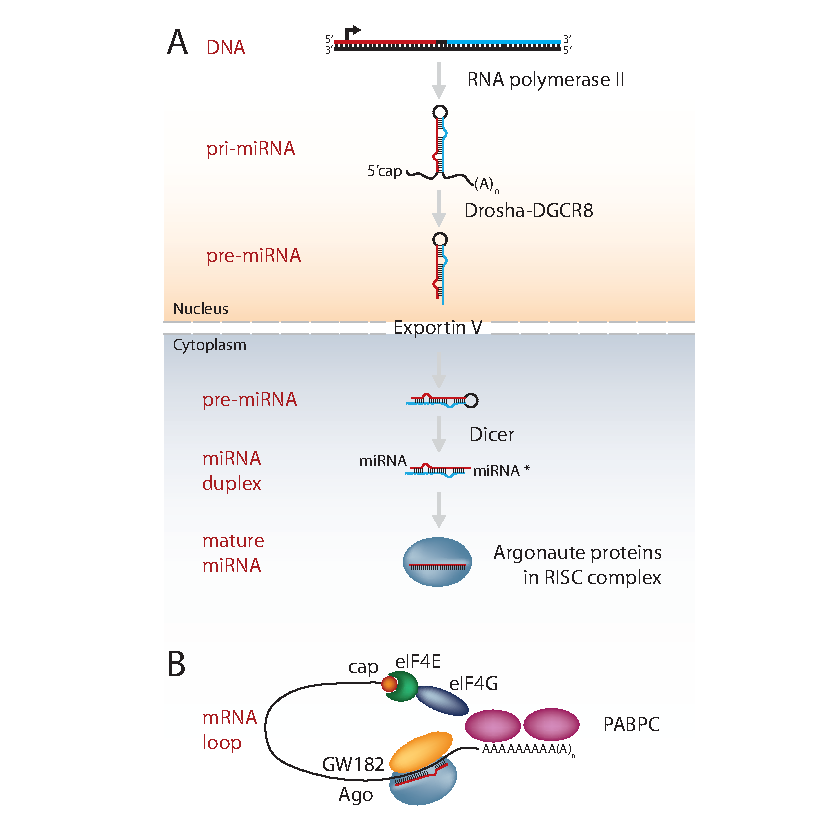
\includegraphics[width=14cm]{miRNAs}
\caption[Biogenesis of miRNAs]{Biogenesis of miRNAs and influence on translation and transcript stability. A. MicroRNA primary transcripts are transcribed by RNAP II into pri-miRNAs with a hairpin loop. After the hairpin has been processed by the Drosha and DGCR8 proteins (Pasha in invertebrates) into pre-miRNAs, it is exported from nucleus by Exportin V. Afterwards, the loop is processed by Dicer, followed by the separation of the mature and the passenger (star) strand. The mature miRNA then binds to the AGO proteins in the RISC complex. B. MicroRNAs control translation and transcript stability by influencing the mRNA loop formation. MicroRNAs lead the RISC complex with GW178 to the transcript. GW178 interferes with the interaction of PABPC with eIF4G which slows down translation. This interference also decreases the number of transcript bound PABPC proteins that protect the polyadenylated tail from exonucleases is decreased, decreasing the transcript stability. \citep{Huntzinger:2011ik}.}
\label{fig:miRNAs}
\end{center}
\end{figure}

The RISC complex contains various Argonoute (AGO)\nomenclature{AGO}{Argonaute} proteins that are guided by small RNAs such as siRNAs and miRNAs to decrease expression of multiple mRNA targets \citep{Meister:2004ha}. The targeting is performed through base pairing between the guide molecule and its target, mainly through a small number of miRNA nucleotides at their $5\textprime$ end termed the ``seed region'' \citep{Lewis:2003ig}. The mature miRNA guides the primed RISC complex to the complementary mRNA loci termed ``target sites'' or miRNA recognition elements (MREs)\nomenclature{MRE}{miRNA recognition elements} \citep{Hutvagner:2001fd}. Target sites are mainly located in the $3\textprime$ untranslated regions (UTRs)\nomenclature{UTR}{untranslated region}, though other parts seem to have importance as well \citep{Bartel:2009fh, InhanLee:2009em}. Depending on the extent of miRNA binding to the target sites, the influence over expression can be quite different. Perfect complementarity leads to direct target cleavage \citep{Yekta:2004ip} and is commonly referred to as RNA interference (RNAi). This is characteristic for siRNAs and is also the main mechanism of miRNAs in plants \citep{Llave:2002uv}. Otherwise, the imperfect miRNA-mRNA binding can influence a large number of targets by both inhibition of mRNA translation \citep{Lee:1993ev, Saxena:2003tk} and decrease of mRNA stability \citep{Orban:2005kj}. Research is still performed to establish the extent and temporal dynamics of each of the previous two processes.
    	
\nomenclature{A, T, G, C, U}{Adenine, Thymine, Guanine, Cytosine, Uracil} 
	
	
	\subsection{MicroRNA mode of action}
	\label{sec:mirna_effects}
	
The main players and processes in the inhibition of mRNA translation by miRNAs have been well described. The miRNAs act on mRNA loop formation (Figure \ref{fig:miRNAs}), whereby $5\textprime$ and $3\textprime$ ends of mRNAs come into proximity, promoting interactions of the $5\textprime$-cap- and the poly(A)-binding proteins and a more efficient translation \citep{Wells:1998jo}. Although miRNAs could act on several stages of translation: initiation \citep{Pillai:2005fx}, elongation \citep{Lee:1993ev, Petersen:2006eb} and protein degradation \citep{Nottrott:2006ju}, not all observations can be fit into a same model. The predominant view is that during the initiation phase proteins from the RISC complex act as $5\textprime$ mRNA cap binding proteins and compete with translation initiation factors \citep{Pillai:2005fx, Kiriakidou:2007il}. This observation has been further confirmed by the lack of miRNA translation silencing upon modification of $5\textprime$ mRNA cap \citep{MotoakiWakiyama:2007fw}, as well as by increased concentration of $5\textprime$ cap binding proteins \citep{Mathonnet:2007ev}. The GW182 protein seems to play a crucial role in this process \citep{Zekri:2009dl}. This RISC complex protein is required for miRNA-mediated gene silencing by competing with the initiation factor eIF4G for binding to the poly(A)-binding protein PABPC.

Besides influencing the translation process, miRNA also decrease the stability of transcripts. The first evidence came from transfection of two miRNAs, miR-1 and miR-124, into cells within which they are normally not expressed \citep{Lim:2005cd}. This  resulted in down-regulation of transcripts containing complementary binding sites. Similarly, levels of miR-430 targets increased in cells in which this miRNA is inhibited \citep{Giraldez:2006gr}. On the mechanistic level, miRNAs seem to promote deadenylation of the mRNA targets, stimulating faster degradation \citep{Giraldez:2006gr, AnaEulalio:2009eh}. This occurs through the previously mentioned GW182 protein that binds miRNAs in the RISC complex and recruits deadenylase complexes to $3\textprime$UTRs of miRNA targets \citep{Braun:2011bo}. Afterwards, the mRNA target is degraded by the enzymes involved in the cellular $5\textprime$-to-$3\textprime$ mRNA decay pathway \citep{BEHMANSMANT:2006fi}. In this pathway, deadenylated \mbox{mRNAs} are decapped by the enzyme DCP2, and ultimately degraded by the major cytoplasmic $5\textprime$-to-$3\textprime$ exonuclease XRN1 \citep{REHWINKEL:2005hp}.

Despite the growing knowledge in the field of miRNA effector functions, it is still unresolved whether miRNA act through translation inhibition or decrease of mRNA stability. In a recent study it was stated that 84\% of changes in protein amount are explicable by the miRNA induced mRNA decay \citep{Guo:2010kh}. On the other hand, translation inhibition can sometimes occur without an influence on expression or even before it \citep{Bazzini:2012jka}. Therefore, it is hypothesised that the same miRNA primed mechanism probably influences independently both mRNA levels and translation \citep{Boland:2011ik}. The function of the intermediary is probably held by GW182 and its two protein binding domains \citep{Fukaya:2011fm} that can influence both expression through PAPBC  \citep{Zekri:2009dl} and translation through the CCR4-NOT proteins \citep{Chekulaeva:2011et} at the same time. 
   
   
 	\subsection{Identification of miRNA targets}
	\label{ref:miRNA_targets}

The mode of action of miRNAs is still disputed, but it is clear that miRNAs influence hundreds of genes at the mRNA and protein levels \citep{Lim:2005cd, Baek:2008ir}. Therefore, identification of individual miRNA targets is performed by an initial identification of potential miRNA-mRNA candidates by genetic, biochemical or computational methods \citep[review in][]{Thomson:2011hc}, which is followed by validation of the predicted interactions \citep[review in][]{Vasudevan:2012cw}. 
	
	Genetic methods for the identification of miRNA-mRNA pairs involve either the mRNA or protein measurements after a perturbation of miRNA level such as over-expression or inhibition Over-expression of miRNAs can be achieved by introducing miRNA hairpin precursors in vectors that produce stable amounts of miRNA \citep{Brummelkamp:2002vx}. However, this approach is problematic since it increases the miRNA amount to artificially high levels that can oversaturate Exportin V or RISC complex proteins and outcompete other miRNAs \citep{Grimm:2006jz}. A further improvement of the system was achieved with lentiviral vectors with pre-miRNAs, the levels of which are more readily controlled \citep{Stegmeier:2005kf}. On the other hand, inhibition of miRNAs is a more controlled way of perturbing miRNAs and can be performed with various silencing approaches. The cells can be transfected with either synthetic miRNA-antisense oligonucleotides like antagomirs \citep{Krutzfeldt:2005ch} and anti-miRs \citep{Elmen:2008iz}, or with vectors expressing antisense miRNA \citep{Ebert:2007ch}.  Both over-expression and inhibition approaches are followed by observations of genome-scale changes either at the expression level through microarrays \citep{Lim:2005cd} and RNAseq \citep{Deng:2011fu}, or at the protein level through stable isotope labelling by amino acids in cell culture (SILAC) \citep{Vinther:2006dk, Selbach:2008hx}. The major drawback of all these methods is that the number of identified mRNA or proteins is quite large and secondary effects of the observed changes cannot be excluded. For that purpose, more specific biochemical approaches have been developed.
	
	The biochemical methods attempt to capture only the primary miRNA targets by immunoprecipitation of RISC proteins and the attached RNAs. Early attempts were directed at the capture of the RISC components \citep{Easow:2007co,Karginov:2007ki} followed by microarray identification of bound RNAs. Though these methods capture RISC-bound RNAs, they are not necessarily native, since these approaches involve a cell lysis step before the RNA assessment. This has been circumvented by exploiting the property of proteins to crosslink bound RNA when submitted to UV in vivo. The crosslinking can be followed by immunoprecipitation (CLIP) to isolate the protein of interest \citep{Ule:2003ja}. The first CLIP method on Ago immunoprecipitates aimed at identifying at the same time both the miRNA and its mRNA target through high throughput sequencing (HITS-CLIP) \citep{Chi:2009ht}. Follow-up methods were developed that surpassed the limits of CLIP such as low efficiency of crosslinking and the lack of the crosslink site information. PAR-CLIP  \citep{Hafner:2010kr} uses photoactivatable ribonucleosides that facilitate cross linking and allows for identification of the cross linking sites through a T to C conversion that occurrs at these loci. On the other hand, iCLIP \citep{Konig:2010ca} identifies the cross link site and reduces the impact of reduced library complexity that occurs through PCR amplification in the usual CLIP procedures. The first step of iCLIP involves a circularisation of all the cross linked reads and is followed by reverse transcription that stops at the cross linking sites where amino acids are attached to RNAs. The sequences therefore start with the cross linking site, and by using barcodes in the sequencing adapters it is also easier to discern the amplification products from the unique sequences. The optimisation of the previously mentioned CLIP methods is still ongoing, but the technology allows for an experimental approach in miRNA target identification that is currently largely independent of computational predictions. 

\begin{figure}[hbtp!]
\begin{center}
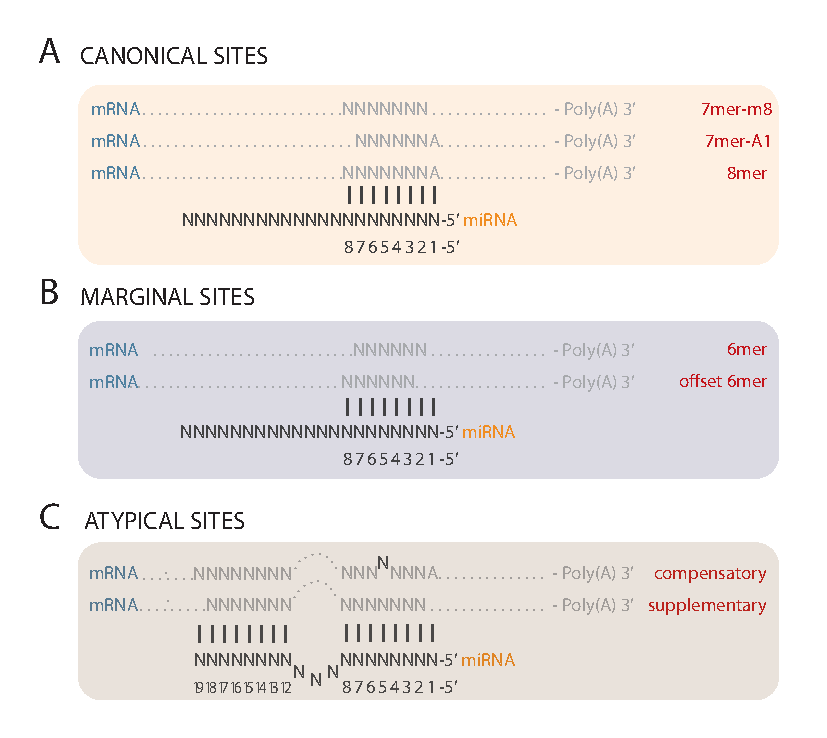
\includegraphics[width=14cm]{seeds}
\caption[Classification of the miRNA-mRNA binding sites]{Classification of the miRNA-mRNA binding sites. The order from top to bottom of the canonical, marginal and atypical categories reflects the decreasing silencing efficiency \citep{Bartel:2009fh}. A. The canonical sites have the strictest binding between the miRNA and mRNA at the seed region (nucleotides 2-8 from $5\textprime$ miRNA end), and can be either 7 or 8 nt long. The most efficient silencers are 8mers, followed by 7mer-m8 and 7mer-A1. B. Marginal sites are 6 nt long and less efficient in silencing, though they are equally abundant. C. The atypical sites rely on binding between miRNA and mRNA outside of the seed region, for more than four (compensatory) or more than three base pairs (supplementary).}
 \label{fig:seeds}
\end{center}
\end{figure}

Computational methods for miRNA target prediction use a combination of sequence, thermodynamic features and conservation of miRNAs and mRNAs to go beyond the limits of experimental procedures. For a computational analysis the sequence of miRNA-mRNA interfaces seems the easiest property to exploit. However, in mammals the position and the extent of binding can vary \citep{Bartel:2009fh}. The majority of pairing between a miRNA and its target is achieved through complementarity with the miRNA $5\textprime$ seed region of nucleotides 2-8 \citep{Lewis:2003ig}. Beside this canonical 7mer pairing, others have been observed (Figure \ref{fig:seeds}) and involve different position and length at the $5\textprime$ end of miRNA, as well as involving other miRNA parts with various degrees of matches and mismatches \citep{MWitkos:2011gj}. Sequence information can also be employed to predict thermodynamic energy of a miRNA-mRNA duplex, or estimate the importance of sequence elements by their conservation in evolution \citep{Enright:2003fj}. 

Multiple algorithms have been developed that use the previously mentioned properties to varying degrees. The first computational target prediction used validated miRNA targets in Droposhila \citep{Stark:2003jb} and was followed by miRanda \citep{John:2004ke}. miRanda used the Smith-Waterman approach \citep{Smith:1981up} to align whole miRNA region with the potential target sites, but weighting results more strongly for matches within the seed region and allowing for mismatches. High-scoring targets were then filtered on the free energy of miRNA-mRNA duplex and conservation predictions. Other methods emphasise different miRNA properties, such as conservation in PicTar \citep{Krek:2005er}, or train their datasets on validated targets as in microT \citep{Kiriakidou:2004kc}. Currently the most popular algorithm is TargetScanS. It requires perfect binding matches within the seed region, in the so called ``canonical sites'' and ``marginal sites'' (Figure \ref{fig:seeds}) \citep{RobinCFriedman:2009km}. It also uses thermodynamics based modelling and performs conservation analysis on human, mouse, rat, dog and chicken \citep{RobinCFriedman:2009km}. However, this algorithm still predicts only 49\% of targets validated from proteomic studies \citep{MWitkos:2011gj}, pointing to the limits of computational miRNA target predictions. On the other hand, methods have been devised that assess enrichment of miRNA targets in the genes lists acquired from the experimental data such as GeneSet2miRNA \citep{Antonov:2009gx},  DIANA-mirExTra \citep{Alexiou:2010bt} and Sylamer \citep{vanDongen:2008cb}. An application of the Sylamer algorithm in detection of miRNA influence on expression datasets will be discussed in Chapter \ref{sec:Chapter4}.
	
After the initial miRNA-mRNA candidates have been established, they have to be validated by one of the following three approaches. In the first one, a cell line is transfected with the bioluminescent protein luciferase, containing the target site for a miRNA of interest in the $3\textprime$ UTR \citep{Zeng:2003ka, Vasudevan:2007by}. The miRNA precursors are then depleted with short interfering RNAs and the target site is confirmed if the luciferase signal was attenuated and if the luciferase with mutated target sites in the $3\textprime$ UTRs is unaffected. After the miRNA levels have been restored by addition of synthetic mature microRNA, the target expression levels are measured to confirm miRNA repression \citep{Vasudevan:2007by}. Similarly, interaction of miRNA with mRNA can be blocked by the previously mentioned antagomirs \citep{Krutzfeldt:2005ch} and anti-miRs \citep{Elmen:2008iz} that can be specifically designed to block only certain mRNAs from miRNA influence. Finally, both the target sites on mRNA can be mutated, followed by a treatment by complementarily mutated miRNAs to rescue the expression levels. 
	
	 	\subsection{The impact of miRNAs}
		\label{sec:miRNA_impact}

Although the first miRNAs have been discovered 20 years ago, it was only in the last 10 years that a vast number of crucial discoveries have been reported \citep{Bartel:2009fh,Vergoulis:2012dk}. This explosion of miRNA related research is largely a consequence of the combination of the rise of new technologies (see Chapter \ref{sequencing}) that gave us sequence information of genomes, high throughput assessment of miRNAs and their targets, as well as computational biology methods  \citep{Lu:2005fx, Ruby:2006bc}. The current release of miRBase (v. 19) \citep{Kozomara:2011es} contains information on more than 25.000 mature miRNAs in 193 species, while over 65.000 entries can be found in Tarbase, the database of validated miRNA-mRNA interactions \citep{Vergoulis:2012dk}. 

MicroRNAs are involved in a multitude of biological process based on their capability to attenuate expression of hundreds of genes at a time \citep{Lim:2005cd, Baek:2008ir}. The effects of miRNAs on individual genes are usually on a small scale \citep{Bartel:2009fh}, but a cumulative effect of such small modifications can result in a change of a developmental plan. For example, introduction of miR-124 to fibroblasts managed to convert them to active neurons \citep{Yoo:2011gt}. This miRNA mode of action can be observed in development \citep[review in][]{Kosik:2009fy}) as well as in other processes such as immune response \citep{Vigorito:2007hk} and cancerogenesis \citep[review in ][]{Zimmerman:2011kc}. Recently, other unexpected miRNA functions have been observed: from exchange of information between cells  \citep{Zhang:2010hd} to receptor-binding in immune response \citep{Lehmann:2012fe}. Such diverse repertoire of functions allows miRNAs to act as both markers of disease \citep[review in][]{Teplyuk:2012dq} and therapeutics \citep{Czech:2011it}. 

Similar to miRNAs, piRNAs were not detected for a long time despite being crucial in silencing of another ubiquitous source of transcripts --- transposable elements. These small non-coding RNAs will be discussed in the next section. 

\section{PIWI-protein interacting RNAs}	
\label{piRNAs}
Transposable elements (TEs) or transposons \citep{McClintock:1950wz} are genomic parasites (``selfish genes'' that are characteristic for all domains of life \citep{Llorens:2007df}. They are characterised by their ability to create their copies elsewhere in the genome (``copy-paste''), or simply relocate their own sequence (``cut-paste''). Alhough it is presumed that some of them are beneficial for genome evolution \citep{Brandt:2005jl}, they induce genome instability by insertional mutations and by providing substrates for additional recombination events \citep{Deininger:2003wk}. Some prokaryotes have developed a defence against them through the CRISPR system (Clustered Regularly Interspaced Short Palindromic Repeats)  \citep{Jansen:2002ve, Mojica:2005hk}. This genetic defence mechanism allows bacteria to store information on viruses and mobile genetic elements it encountered and uses it to target their DNA in the future \citep{Bolotin:2005gj}. Other defence mechanism involve RNAi systems with AGO proteins  \citep{Song2:2004ge} that have also been implicated in the control of mobile genetic elements from prokaryotes, unicellular organisms to plants and animals  \citep{Makarova:2009kq, Djikeng:2001um, Hamilton:1999dy, Aravin:2003ht}. Some species of plants \citep{Mosher:2008ef} and animals \citep{Brandt:2005jl,Aravin:2008kz} employ DNA methylation to control transposons, since it can silence the expression of chromatin regions \citep{McGhee:1979tz}.

	Animals use small non-coding piRNAs and DNA methylation to target transposable elements, but their action is restricted to the germ-line cells. The germ-cell genomes need special protection since their information is directly transmitted to the offspring. Furthermore, in some species whole genomes undergo demethylation that derepresses silenced TEs \citep{Tada:1997kw,Mayer:2000dl}. In the following section general properties and biogenesis of piRNAs will be discussed in greater detail.
	
\subsection{Discovery of piRNAs}

PIWI-interacting RNAs were first described as ``repeat-associated small interfering RNAs'' (rasiRNAs) in 2001 based on their conserved function in control of retrotransposons in several species: \textit{Trypanosoma brucei} \citep{Djikeng:2001um}, \textit{Arabidopsis thaliana} \citep{Hamilton:1999dy} and \textit{Drosophila melanogaster} \citep{Aravin:2003ht}. The rasiRNAs are now considered just a subclass of the piRNAs specific for the regulation of transposable elements \citep{Brennecke:2007kfa}. After the definition of piRNAs as a novel class of non-coding RNAs in 2006 \citep{Vagin:2006cs, Aravin:2006p384, Watanabe:2006ij, Lau:2006ka, Girard:2006gu}, other characteristics have also been confirmed. 

First, their length was 24-31 nt, which made them separate from existing siRNAs and miRNAs that are often processed with Dicer proteins that are currently considered dispensable for piRNA production \citep{Vagin:2006cs}. Furthermore, piRNAs exhibit a strong propensity for a $5\textprime$-Uridine, characteristic of the \mbox{RNAse III} enzyme processing \citep{Aravin:2003ht}. Their $5\textprime$ end contains a monophosphate similar to other small non-coding RNAs. On the other hand, their $3\textprime$ end is specifically $2\textprime$-O-methylated, in contrast to animal miRNAs and siRNAs \citep{Kirino:2007iv}. Another property of piRNAs is that, when their sequence is aligned to the genome, they cluster to a set of genomic loci that can span up to few hundred kilobases \citep{Aravin:2007hw}. Finally, piRNAs are exclusively processed by the PIWI (P-element Induced Wimpy Testis) clade of the Argonaute protein family \citep{Aravin:2006p384}.

\subsection{Proteins involved in piRNA processing}
\label{sec:piwiprot}
PIWI (P-element induced wimpy testis)\nomenclature{PIWI}{P-element induced wimpy testis} proteins were first discovered in \textit{D. melanogaster} while examining germ-line stem cells through P-element mutagenesis \citep{Lin:1997un}. Mutations of these genes cause arrests in spermatogenesis and the consequential reduced size of gonads. Similar to other Argonaute proteins, PIWI homologues contain three domains,  PIWI, MID and PAZ (an abbreviation for Piwi/Argonaute/Zwille), essential for piRNA processing \citep{Cerutti:2000ut, Song:2004ge}. The PIWI domain contains the RNAase H fold that in some proteins performs endonucleolytic activity, also  termed ``slicing'' \citep{Song:2004ge, Parker:2005de, Gunawardane:2007ka}. Jointly, MID and PIWI domains recognise the $5\textprime$ end of single-stranded RNAs (ssRNAs) \citep{Boland:2011ik}, while the PAZ domain recognises and binds the $3\textprime$ end of ssRNAs \citep{Lingel:2004fs, Simon:2011dg}. 

Highly conserved homologues of PIWI were found in other animals to be essential for the formation and maintenance of germ-line \citep{Cox:1998ts} as well as the control of transposable elements (TEs) \citep{Kalmykova:2005cj}. In \textit{C. elegans} the TE regulatory function of piRNAs is performed by 21U RNAs \citep{Ruby:2006bc} as well as 22G RNAs \citep{Gu:2009cd} that are processed by AGO homologues termed Wagos. The majority of piRNA biogenesis and function was elucidated in \textit{D. melanogaster} that contains three piRNA processing proteins: Argonatue 3 (Ago3), Aubergine (Aub) and Piwi \citep{Brennecke:2007kf}. The piRNA biogenesis and function in vertebrates also involves multiple PIWI proteins. In zebrafish (\textit{Danio rerio}) there are two (Ziwi and Zili) \citep{Houwing:2008fm}, while mammals contain three, such as Mili, Miwi and Miwi2 in mouse \citep{Girard:2006gu, Aravin:2006p384, Carmell:2007fi}. 

The individual properties of mouse PIWI homologues are crucial for our understanding of piRNA biogenesis and function, especially since they prefer different piRNA species, cell compartments, developmental stages and tissues. First of all, PIWI homologues are associated with piRNAs of different length, as defined by 25-27 nt species for Mili, 29-31 nt from Miwi and 27-29 nt for Miwi2 \citep{Aravin:2006p384, Aravin:2008kz}. Similar to \textit{D. melanogaster}, these proteins are mainly located in non-membranous perinuclear granules \citep{AlexeiAAravin:2009cu}. Mili is enriched in the small and numerous pi-body granules that are also known as �the intermitochondrial cement� (IMC)\nomenclature{IMC}{intermitchondrial cement} \citep{Aravin:2008kz}. Miwi2 is concentrated in a small number of large piP-granules that contains many enzymes of the mRNA processing machinery \citep{Balagopal:2009gda, AlexeiAAravin:2009cu}. Miwi is expressed only after birth and localises together with Mili to the adult-specific version of previously mentioned perinuclear granules called �chromatoid bodies� (CBs), characteristic of the adult spermatocytes \citep{Kojima:2009eb}. All PIWI proteins are coupled in their granules with multiple proteins of the Tudor family, that are responsible for their localisation and target specificity \citep{Wang:2009cq, Siomi:2010jk}. As an exception to the localisation in the perinuclear granules, Miwi2 can also be found in the nucleus \citep{Aravin:2008kz, Brennecke:2008p641}, where it is involved in methylation of the genomic loci of repeat elements \citep{KuramochiMiyagawa:2008jn}. Furthermore, while Miwi2 is specific for embryonic testes and Miwi for the adult ones, Mili is expressed throughout the development and produces both the embryonic (pre-pachytene) piRNAs involved in transposon control and the adult (pachytene) piRNAs of unknown function (Figure \ref{fig:spermatogenesis}) \citep{Aravin:2008kz}. Finally, PIWI proteins in mouse are mostly restricted to the male germ-line, though Mili can also be found in the ovaries \citep{KuramochiMiyagawa:2001wn}. Several recent studies reported piRNA-sized RNAs in other somatic tissues \citep{Yan:2011ff, Lee:2011da} as well as in cancer tissues \citep{Siddiqi:2012dp}. However, the piRNA somatic functions are yet to be determined.


\begin{figure}[hbtp!]
\begin{center}
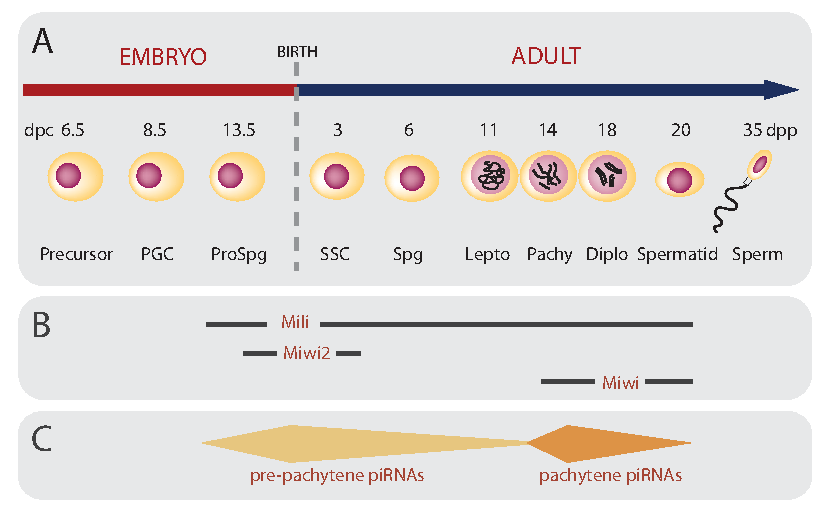
\includegraphics[width=14cm]{spermatogenesis}
\caption[Expression of piRNAs and PIWI proteins in spermatogenesis]{Expression of piRNAs and PIWI proteins in spermatogenesis. A) Formation of a mature sperm involves multiple differentiation steps in embryonic and adult development. Embryonic precursor cells of germ line develop 6.5 days \textit{post coitus} (dpc) and migrate to the gonads to form primordial germ cells (PGC). These then differentiate into male prospermatogonia (ProSpg) or gonadocytes before birth. Three days after birth (\textit{post par item} dpp), gonadocytes form spermatogonial stem cells (SSC), a testis specific pool of stem cells that differentiate into spermatogonia. Spermatogonia undergo mitosis to produce spermatocytes. These undergo meiosis, whereby chromosome condense in leptotene (Lept), recombine in pachytene (Pachy) and separate in diplotene (Diplo). After the second round of meiosis, round spermatids are formed which mature into sperm. B. Expression of Mili, Miwi and Miwi2 throughout the spermatogenesis. C. Production of pre-pachytene and pachytene piRNAs in relation to different stages of spermatogenesis and presence of PIWI proteins.}
 \label{fig:spermatogenesis}
\end{center}
\end{figure}


\subsection{piRNA biogenesis}
\label{sec:pingpong}
The biogenesis of piRNAs is related to its function in silencing of transposable elements (TEs) and occurs in three steps: transcription from mainly intergenic loci, export out of the nucleus and processing into oligonucleotides and amplification by the PIWI proteins \citep{Aravin:2006p384}. 

Initially, primary piRNAs transcripts are presumed to be transcribed from a set of genomic loci by an unknown RNA polymerase. Most piRNAs seem to map to the genome in clusters with a strand bias, pointing to biogenesis from long primary transcripts \citep{Aravin:2006p384}. These clusters are conserved in their chromosomal arrangement (synteny), but share no sequence similarity \citep{Girard:2006gu}. In mammals, there are several differences between the embryonic (pre-pachytene) and adult (pachytene) clusters. First, pre-pachytene and pachytene clusters show little overlap in their genomic loci. Second, the pachytene clusters contain a higher proportion of uniquely mapping piRNAs (80\% vs 60\%) and are depleted of transposable elements \citep{Betel:2007p580}. Finally, the majority of pachytene piRNAs are distributed over a smaller number of clustered regions, but with a greater concentration of piRNAs and a higher occurrence of sequence that are antisense to transposons \citep{Aravin:2006p384}. However, the current evidence for primary transcription is still only indirect and comes from mapping of piRNA sequences to their genomic locations.

The post-transcriptional steps of piRNA biogenesis are not well defined. It is presumed that single stranded primary transcripts are exported out of the nucleus and recognised by endo- and exonucleases such as Zucchini \citep{Nishimasu:2012cea, Ipsaro:2012ii}. Little is known about this step, except that processing probably occurs in perinuclear granules \citep{Siomi:2011gh}. Dicer has also been excluded from the process, since in \textit{D. rerio} it is not required for piRNA production and usually processes double stranded substrates \citep{Vagin:2006cs}.  After the processing by Zucchini that cuts specifically single-stranded piRNA precursors, the nascent fragments are taken by he PIWI proteins \citep{Siomi:2011gh}. Some PIWI proteins such as Ago2 in \textit{D. melanogaster} or Mili in mouse have a preference for the sequences with a first Uracil base  \citep{Brennecke:2007kf}. In the next step, the 3$\textprime$ end is trimmed by the exonucleases and methylated on the 2$\textprime$-O position to produce primary piRNAs. The current model does not account for the function of helicases (Armitage in \textit{D. melanogaster} and Mov10L1 in mouse) that are also required for piRNA biogenesis \citep{Saito:2010kq, Frost:2010jn, Zheng:2010ho}. 


\begin{figure}[hbtp!]
\begin{center}
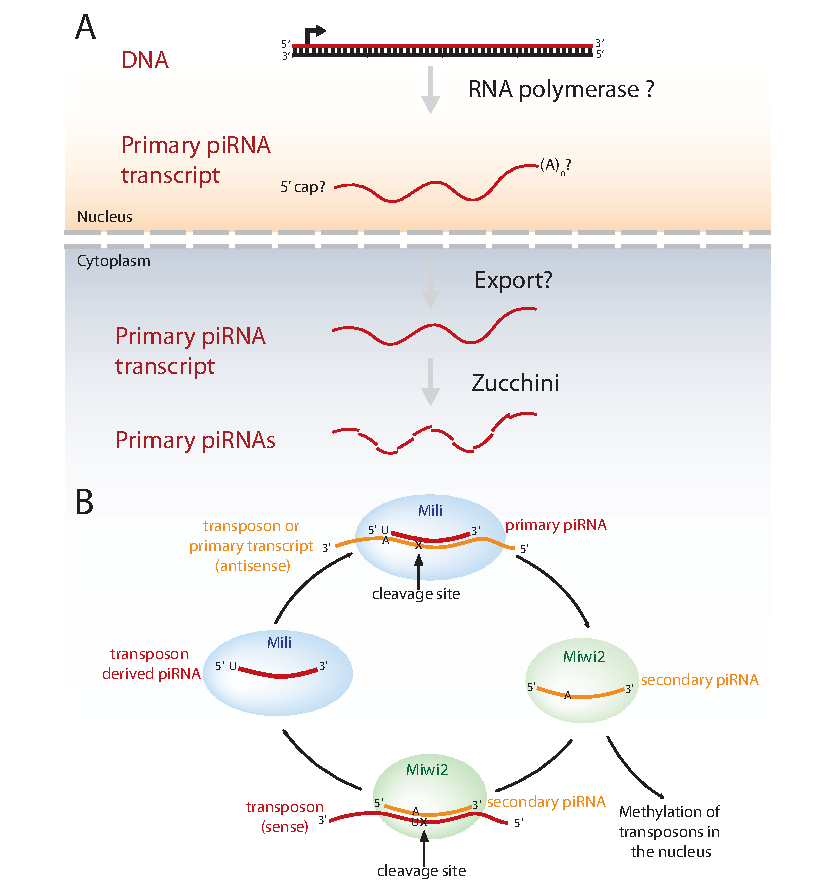
\includegraphics[width=14cm]{piRNAs}
\caption[Biogenesis of piRNAs]{The current model of mammalian piRNA biogenesis. Primary piRNAs prime Piwi proteins and guide them to transposon cleavage or methylation of transposon genomic loci. A. The primary precursors are transcribed by an unknown RNA polymerase and exported out of nucleus. The endonuclease Zucchini then cuts these single stranded piRNA precursors into oligonucleotides. B. The ``ping pong'' piRNA amplification cycle. The piRNAs with $5\textprime$ U are adopted by Mili that cleaves either the antisense transposon transcript or an antisense primary precursor. This cleavage event produces of a secondary piRNA with a tendency for 10' A. \citep{Brennecke:2008p641, Gunawardane:2007ka}. The secondary piRNAs target transposon RNAs that are generated from piRNA clusters. Cleavage of such transcripts reproduces original primary piRNAs that target antisense transposons or antisense primary transcripts. Miwi2 can also use the secondary piRNAs to target transposon loci in the nucleus.} 
 \label{fig:piRNAs}
\end{center}
\end{figure}

After the primary piRNAs have been formed, an amplification cycle termed ``ping-pong'' is supposed to create secondary piRNAs (Figure \ref{fig:piRNAs}). Sequencing of piRNAs revealed that the piRNAs on the opposite strands often overlap at their first 10 nucleotides, resulting in the propensity for U as the first nucleotide of a sense piRNA and A as the 10th nucleotide of a paired antisense piRNA. A mechanism was proposed by which Ago3 and Aub, two \textit{D. melanogaster} proteins in turn take piRNAs, cut transposon sequence, and use the nascent secondary piRNAs to cut more primary transcripts. The same mechanism was presumed in mice, with Mili and Miwi2 assuming the role of Ago2 and Aub \citep{Aravin:2007hw}.  By this model, Mili is primed by the piRNAs which are in the same sense as transposons. In combination with an unknown exonuclease to cut out the extra TE parts, this would create a secondary piRNA that commonly have Adenine at the 10th position. Since the sequences obtains from Miwi2 immunoprecipitations are enriched for these secondary piRNAs, it is presumed that it performs the second part of the cycle, by cutting the antisense transposon or primary piRNA transcript \citep{Aravin:2008kz}. This in turn would create more secondary piRNAs to cut transposons in an amplification loop. 
	The current ``ping pong'' model in mouse has several limitations. First of all, the �ping-pong� signature of 10 nt overlap between sense-antisense piRNA pairs is missing in adult testis \citep{Beyret:2012gc}. Second, Miwi2 is not present in the adult stages of spermatogenesis, when the pachytene piRNAs are being formed \citep{KuramochiMiyagawa:2008jn,Carmell:2007fi,Girard:2006gu}. Finally, Miwi2 is enriched in physically separate granules from Mili \citep{AlexeiAAravin:2009cu}.  


	\subsection{The function of piRNAs in mammals}
\label{piRNA_function}
The details of piRNA biogenesis have mostly been observed on embryonic piRNAs, while little is known on formation of the adult piRNAs. The same discrepancy applies to our knowledge of piRNA function during the course of spermatogenesis. 

The pre-pachytene piRNAs silence transposable elements (TEs)\nomenclature{TE}{transposable element}  in the embryonic stages of development. In animals  there are multiple types of TEs \citep{Jurka:1998vd}. The first ones are the Class I retrotransposons which contain an RNA during their cycle. Some of them form virus like particles in the cytoplasm and contain long terminal repeats (LTR)\nomenclature{LTR}{long terminal repeat}  that are used to insert their genetic sequences back into the host \citep{Shank:1978ub}. These LTRs, such as intracisternal A-particles (IAPs) \citep{Kuff:1983vj} contain a retrotransposase enzyme that allows for an increase in copy number by producing extra DNA copies from an RNA template \citep{Weiner:1986io}. Other Class I retrotransposons such as long and short interspersed nuclear elements (LINE and SINE)\nomenclature{LINE}{long interspersed nuclear element} \nomenclature{SINE}{short interspersed nuclear element} do not contain LTRs. LINE elements exit the cell and form ribonucleic particles, but SINEs do not code for proteins and use the machinery of LINE to increase the number of their copies. The class II or the DNA transposons \citep{Fraser:1983vn} code for a transposase \citep{Heffron:1979vza} that allows their movement around the genome, but they do not actively replicate. 

What all of the previously mentioned Class I transposons have in common is that they become active during the whole-genome demethylation that occurs during spermatogenesis \citep{Hajkova:2002ur, Walsh:1998cf}. The repression is mediated by piRNAs either by the endonucleolytic activity of PIWI proteins on transposon transcripts \citep{Aravin:2007hw} as described in Section \ref{sec:embryopingpong} or by silencing of their genomic regions through methylation of CpG islands \citep{KuramochiMiyagawa:2008jn}. Miwi2 performs methylation of TE genomic sites via a class of methylases called DNA methyltransferases (DNMT) \citep{Aravin:2008kz}. DNMT3L is a DNA methyltransferase that is germ line specific  and essential for methylation of transposons \citep{Bourchis:2004to}.

	Although the adult piRNAs were the first ones to be discovered, their biogenesis and function remain largely unknown. They are also formed from primary cluster loci, but their clusters are smaller, contain more piRNAs and are depleted of repeat regions \citep{Aravin:2007hw}. The details of their export and processing are also unknown and they seem seem to be amplified by the PIWI proteins \citep{Grivna:2006p577}. The non-repeat function of some piRNAs has been hypothesised to relate to chromatin, mainly through their involvement in the methylation process \citep{Olovnikov:2012ii}.  In \textit{D. melanogaster} clusters are often located in telomere and centromere regions, though their translocation to other regions did not have any effects on spermatogenesis \citep{Muerdter:2012jw}. A crucial step closer to identifying the function of pachytene piRNAs is to investigate the mechanism of their transcription and their evolution on a transcriptomic and epigenetic level (Chapter \ref{sec:chapter_piRNAs}). To that end, a set of sequence-based techniques has been employed, which will be discussed in the next section.


\section{Sequence-based technologies in genomics and transcriptomics}
\label{sequencing}
	Our current understanding of the biogenesis and function of non-coding RNA was largely possible due to the developments in the field of genomics. However, the path to the fully annotated genomes, such as the ENCODE\nomenclature{ENCODE}{encyclopaedia of human DNA elements} encyclopaedia of human DNA elements took several important steps. 
	
	The first genome sequenced was of $\Phi$X174 bacteriophage in 1977 \citep{Sanger:1977vp}. Genome size was a major technical limit and even small genomes such as  \textit{Escherichia coli} \citep{Blattner:1997ha} and \textit{Saccharomyces cerevisiae} \citep{Goffeau:1996eu} took a further 20 years to sequence. The first attempts to gain genome-wide information on  mammalian genomes was performed in 1990, with expressed sequence tags (EST) providing sequence information on 600 human protein-coding genes at once \citep{Adams:1991ua}. This information was used to build computational tools to annotate the next large sequencing endeavour, human chromosome 22 in 1997 \citep{Dunham:1999ib}, as a part of the Human Genome Project that started in the late 1980s \citep{Watson:1990ub}. The first draft of the human genome took more than 10 years before after the final version was publicly available and that required drastic changes in sequencing technology and gene prediction \citep{lander:2001hk}. 
	
	The focus then shifted to annotation of the genomic elements, which resulted in the ENCODE pilot project, annotating 1\% of the total human genome in 2007 \citep{Birney:2007fu}, and the full genome 5 years later \citep{Consortium:2012db}. The main techniques in analysis of sequence composition and gene expression that allowed for these scientific breakthroughs will be discussed in the next section.

	\subsection{Sequencing technologies}
	
	The principles of sequence-based technologies are grounded in the properties of nucleic acids that make them efficient information carriers \citep{Church:2012fd}. The first one is the accurate information transfer from one strand of DNA or RNA to the complementary one, due to the rules of base pairing. The second is the easy information amplification for increased signal-to-noise ratio, due to the ability of double strands of DNA to separate and re-hybridise under high-low temperature cycles or enzymatic treatment. These two properties in combination with various protein catalysts and chemically modified nucleotides are still the basis for the majority of methods for sequence identification and quantification \citep{Morozova:2008cn}.

	\subsubsection{The early days}
	\label{PCR}
	
	Maxam and Gilbert were the first to develop a method for DNA sequencing in 1977 \citep{Maxam:1977vy}. Their method involved separation of a sample into four parts and incomplete chemical degradation of one out of four nucleotides in each of the subsamples. This was followed by the separation of resulting $5\textprime$ radioactively labeled DNA fragments on a polyacrylamide gel, whereby fragment length pointed to the position of individual nucleotides in the sequence. Similarly, the Sanger method used the length of fragments created by DNA polymerase, with four different dideoxy nucleotide homologues stopping the polymerisation at their inclusion sites \citep{Sanger:1977vp}. Furthermore, modifications of the Sanger method were later developed, whereby different fluorescent dyes were tagged to the dideoxy nucleotides themselves \citep{Smith:1986ie}. This approach allowed for automation of the process by combining the four subsamples for each nucleotide, and detecting the fluorescent colour of each of the fragment band as it passed through a high sensitivity fluorescence detector. The sequence was determined from the temporal order of peaks corresponding to each of four different fluorescent dyes, and the computers were used to deconvolute the signal. Finally, the sequencing was further speeded up and automated by use of capillary electrophoresis instead of gels, which allowed for parallel analysis of up to 96 samples \citep{Blattner:1997ha}.  
	
	\subsubsection{Second generation sequencing}
	\label{sgs}
	The previous approaches were used to sequence genomes of major model organisms, from Bacteria \citep{Blattner:1997ha} to human \citep{lander:2004bm}, but it was the development of modern techniques of �second� or �next� generation sequencing that allowed for a drastic increase in sequencing speed and reduction in cost \citep{Metzker:2009ew}. These methods do not evaluate sequence composition by fragment sizes, but by the individual polymerisation additions for each of the nucleotides to the complementary strand of sequenced DNA. 
	
	The first method was pyrosequencing, developed in 1996 \citep{Ronaghi:1996jt}. Sample DNA with adapter sequences were added to streptavidin-coated magnetic beads in quantities that promoted ligation of only one sequence to a bead. The template on each bead was then amplified through a polymerase chain reaction (PCR)\nomenclature{PCR}{polymerase chain reaction}  (see Chapter \ref{PCR}). In the next step, each of the four nucleotides were added and removed in turn, in the presence of a mixture of enzymes required for the DNA polymerase reaction and photo-detection. Successful incorporation of a nucleotide releases a pyrophosphate which activates a photo-reactive moiety in a quantitative manner \citep{FakhraiRad:2002ke}. This methodology is the basis for the commonly used 454 sequencing system, whereby the individual beads with a sample are spread over small wells and individually pyrosequenced, allowing for genome-scale analyses \citep{Margulies:2005gw}. 
	
	The Illumina method shares this ``sequencing by synthesis'' approach with 454 technology, but several differences have made it more popular. The sequencing is performed on solid surfaces, not  beads, and this allows for a much larger number of sequences to be evaluated in parallel \citep{Bentley:2008eo}. This is achieved by initial attachment of DNA randomly to a flow cell, followed by amplification that creates clusters of up to 1000 identical DNA sequences. Next, the nucleotides are added in turn, but unlike 454 where incorporation of copies of a nucleotide in the same cycle are a possible source of error, the Illumina system uses nucleotides as polymerisation terminators. This ensures that only a single nucleotide can be incorporated in time. The attached fluorescent dyes are then detected by the instrument for each cycle of synthesis. Furthermore, the initial limit of 18 gigabases (Gb) per Illumina Genome Analyzer run \citep{Metzker:2009ew} was increased to 600 Gb for the HiSeq method, with the maximum length of reads now at 100 bp \citep{Liu:2012hw}. This is several orders more processive than 454 (0.45 Gb per run), but the length of 454 reads (330 nt) allows for better assessment of sequenced regions with gaps and repeats \citep{Metzker:2009ew}. 
	
	Finally, SOLiD sequencing is the third largest sequencing platform. Instead of using sequencing by synthesis, it performs DNA sequencing based on ligation of fluorescently labeled probes to the DNA sequence \citep{McKernan:2009cl}. After amplification of sequences on beads similar to 454, the beads are deployed on flow cells. A complex set of overlapping primers is then added to guide the binding of probes, labeled based on the nucleotide content of their first two bases. Ultimately, for each nucleotide of the sequence two nucleotides are assessed at the time, whereby each nucleotide is effectively sequenced twice. This allows for higher accuracy of detected sequences, which makes this technology more suited for variation studies. However, the time required for sequencing is on the order of weeks and the reads are shorter than in the other methods (50 bp) \citep{Liu:2012hw}. 
	
	\subsubsection{Applications of the second generation sequencing methods}
	\label{SGS_applications}
	
	The decreasing cost of the sequencing methods allowed for their wide usage beyond pure sequence determination and a selected few will be discussed in more detail.
	
	RNA-seq experiments allow for a quantitative assessment of the amount of gene expression as well as the detection of novel transcripts. The technology is based on extraction of RNAs either by poly(A)-enrichment or rRNA depletion of total cellular RNA content, followed by cDNA synthesis and second generation sequencing \citep{Morin:2008gf}. The number of sequences detected can be used to estimate a broad range of transcript expression, while in the same time detecting both coding and non-coding transcripts. 
	
	ChIP-seq (CHromatin ImmunoPrecipitation followed by sequencing)\nomenclature{ChIP-seq}{chromatin immunoprecipitation followed by sequencing}  technology has been widely used in the fields of expression regulation and epigenetics, since it detects the DNA-protein interaction sites of DNA-binding proteins \citep{Barski:2007gh}. In the first step of this methodology proteins are crosslinked with bound DNA, typically with formaldehyde. This is followed by immunoprecipitation of the target protein, and sequencing of the unlinked DNA with second generation sequencing. 
	
	Furthermore, these methods can also be used to detect interactions of close fragments of DNA, with a range of techniques jointly known as ``chromosome conformation capture'' \citep{Dekker:2002ub}. These techniques are also based on crosslinking of DNA strands with proteins, although this time a protein is involved in interaction with two DNA sequences. The treatment of such DNA-proteins complexes with a restriction enzyme digestion leaves short sequences attached to a protein.  In the next step, these short sequences are ligated and detached from the protein. The initial methods such as  3C \citep{Dekker:2002ub}, 4C \citep{Zhao:2006jn} and 5C \citep{Dostie:2006kx} amplified the ligated DNA with specific primers, allowing for identification of DNA interactions of only specific loci. However, the recently developed HiC \citep{LiebermanAiden:2009jz} protocol captures DNA-DNA interactions on a genome-scale level. The specificity of capturing only crosslinked DNA is achieved by using biotin in the ligation step, and is followed by a capture with spretavidin, second generation sequencing and a complex computational analysis. 
	
	Finally, the bisulfite sequencing method captures the methylation state of a genome \citep{Ball:2009kh}.  Addition of a methyl group to cytosine residues of the CpG dinucleotides has been implicated in transcriptional repression. Treatment of DNA with bisulfite introduces specific changes by converting non-methylated Cytosine residues to Uracil. After sequencing, these changes that point to methylation sites can be observed by a comparison with the original genomic sequence. 
			
	\subsubsection{Third generation sequencing}
	
Despite their broad usage, current sequencing methods have several inherent problems. They depend on PCR amplification of sequences to clusters, either on beads or flow cells, which introduces further biases and reduces complexity of the sample  \citep{Schadt:2010cp}. Furthermore, they produce large quantities of redundant, overlapping data with sequences of short length. In the last few years there has been a decrease in the time and cost of sequencing \citep{Metzker:2009ew, Liu:2012hw}, but single molecule sequencing (SMS) techniques are expected to bring it down even more \citep{Pushkarev:2009cw}. SMS intends to acquire sequence information from a single molecule of DNA or RNA as it passes through a detector in multiple ways. The Helicos system images polymerisation of the second strand in real time with a defined primer, a modified polymerase and fluorescently labeled nucleotide analogues, producing short reads of 25 nt \citep{Harris:2008gf}. Single molecule real time sequencing (SMRT) by Pacific Biosciences directly observes polymerisation of a single molecule of DNA by observing the release of a fluorescent dye as it leaves the tiny polymerisation chamber \citep{Eid:2009kv}. Finally, the Oxford nanopore system detects individual nucleotides once they are cleaved from the individual DNA molecules and pass through small pores. All of these technologies are still in development, but once technical issues are solved the low cost that they promise and the amount of the sample needed will likely allow them to dominate the field of nucleic acid sequencing

	\subsection{Gene expression profiling}

The previously mentioned sequencing approaches provide mostly just the bare sequence of the DNA or RNA in question. The second generation sequencing crossed this line from the qualitative to quantitative analysis of sequences, since the number of times a sequence appears in the output can be used as a measure of the abundance of the template sequence. However, the majority of gene expression quantification is still performed with non-sequencing technologies due to their low cost and the well established analysis protocols.

	\subsubsection{The early days}

	The first technique to evaluate gene expression levels was the Northern blot, developed in late 1970s \citep{Alwine:1977uz}. The procedure involved separation of mRNAs based on their size with gel electrophoresis, followed by hybridisation of radioactively fluorescently tagged oligonucleotide probes for the sequence of interest. The technique allows for both qualitative and quantitative evaluation of expression, and is still in use today for its simplicity. In 1983 the polymerase chain reaction (PCR) method was developed that revolutionised molecular biology by allowing for amplification of minute amounts of genetic material \citep{Saiki:1985to, Mullis:1990wx}. The PCR reaction amplifies DNA or RNA by using thermostable polymerases that remain active despite multiple cycles at room temperature ssDNA-primer annealing and dsDNA polymerisation and high temperature and dsDNA separation (``melting''). PCR can be used to detect expression through the use of quantitative real-time PCR (qRT-PCR) technique \citep{Holland:1991tc}. In these methods, a dye is added that fluoresces upon binding to dsDNA, or the degradation of a part of probe releases an otherwise quenched fluorophore. The amount of fluorescence is then compared to a control for each cycle, or a relative amount to an internal reference gene can be measured. Despite being the gold standard to measure RNA expression even today, the major drawback is its inability to measure expression of all cellular transcripts at once.

	\subsubsection{High throughput methodologies}
	\label{microarrays}
	The first step in evaluation of gene expression on a genome scale level was the introduction of expressed sequence tags (EST) in the 1990s \citep{Adams:1991ua}. ESTs are small DNA sequences (300-500 nucleotides long) generated by sequencing total mRNA of all expressed genes in cells of interest. Messenger RNAs were first converted to complementary DNA (cDNA)\nomenclature{cDNA}{complementary DNA}  with an enzyme reverse transcriptase and then sequenced from both the $5\textprime$ and $3\textprime$ end. This technique allowed, for the first time, cataloguing of species and tissue specific transcriptomes. Furthermore, the unique ESTs were the basis of the Unigene database, that contains unique identifiers for all the known genes \citep{Boguski:1995kg}. Finally, besides being an early gene finding tool, the EST libraries were also used for the first two whole genome expression platforms; serial analysis of gene expression (SAGE) and DNA microarrays.
	
 	SAGE is a genome wide expression assessment platform that can provide information on all expressed mRNA in a sample at once \citep{Velculescu:1995ik}. In the first step, small sequence tags (\textless30 bp) are obtained from $5\textprime$ or $3\textprime$ part of the expressed transcript. Next, the tags are concatenated together and sequenced. In the final step the expression level of each transcript is quantified based on the frequency of each of the observed tags. With the help of EST libraries, expression of individual genes was assessed, but this technique was soon replaced by cheaper and less labour intensive DNA microarrays.
	
	Despite the rise of second generation sequencing methods, DNA microarrays (or DNA chips) still provide a robust approach in evaluation of mRNA expression \citep{Malone:2011ib}. The method is based on binding of a sample of mRNAs to complementary cDNA or ssDNA  oligomers (probes) that were previously attached to a solid glass or plastic surface \citep{Schena:1995tu}. There are several modifications to the basic idea. In the two-sample protocol, short complementary cDNA of interest is spotted on arrays and bound by two samples that are tagged with either green or red fluorescent marks. The ratio of green to red fluorescence evaluates relative amounts of expressed mRNA for each of the samples \citep{Shalon:1996uf}. In the second type, the oligonucleotide microarrays, the probes are synthesised on a silicon or glass surface (array or chip) and are 60 (Agilent) \citep{Blanchard:1996go} or 25 (Affymetrix) \citep{Lipshutz:1999ez} nucleotides long.  In this approach, the mRNA sequences are added to the oligonucleotide samples without a second color, and their expression is compared across conditions. The accuracy of binding is measured against binding to oligonucleotides with a mismatch in the middle of the sequence. The third approach is used is the BeadArray technology \citep{Oliphant:2002vf}. In this approach the probes are attached to beads, and deployed randomly on arrays to be bound by labeled complementary RNA (cRNA). The detection of the probe location is performed through a specific 29 nt ``address'' at the $5\textprime$ end of the probe.  
	
	In summary, microarrays are still the method of choice for the evaluation of the coding transcripts, since they are the statistically well defined system and inexpensive compared to the sequencing technologies \citep{Malone:2011ib}. However, the problem is that they can only detect previously described sequences (usually protein-coding ones) and are not capable to detect novel transcripts. Furthermore, they cannot be used to quantify absolute gene expression, but can only provide an expression value relative to a reference sample.  A modification of the DNA microarrays called tiling arrays circumvents this problem by placing on multiple chips oligomeric sequences that cover an entire genome \citep{Bertone:2004gj}. Tiling arrays have been used in multiple other methods: to detect regions bound by immunoprecipitated DNA-binding proteins (chip-ChIP) \citep{Horak:2002uj}, chromatin methylation (MEDip-ChIP) \citep{Palmke:2011hz} or chromosomal duplications in cancer (CGH)\citep{Pinkel:1998da}. However, despite the statistical power and multiple applications, the cost of tiling arrays for mammalian genomes is prohibitive, where they are already replaced by the second generation sequencing methods.

\nomenclature{ssDNA}{single stranded DNA} 
\nomenclature{dsDNA}{double stranded DNA} 
\nomenclature{ssRNA}{single strandedRNA} 
\nomenclature{dsRNA}{double stranded RNA} 

\newpage
\section{Aims of the analyses}

During the course of my studies, my aim was to investigate properties of non-coding RNAs from a perspective of computational biology. Three types of RNAs were the focus of method development and data analysis: pachytene piRNAs, pre-pachytene piRNAs and microRNAs. 

Unlike pre-pachytene piRNAs, which are largely involved in the regulation of mobile genetic elements, the function of the pachytene piRNAs remains elusive \citep{Siomi:2011gh}. These piRNAs are associated with Mili and Miwi only, and are expressed later in spermatogenesis in exceptionally large amounts \citep{Aravin:2006p384}. They seem to contribute greatly to the germinal granules or nuage where they are stored together with other haploid mRNA transcripts \citep{Meikar:2010jm}. Most pachytene piRNAs seem to be produced from long primary transcripts \citep{Aravin:2006p384}, but little is know about their transcription properties as well as their mechanism of formation.
The aim of this aspect of my studies was to define genomic features and evolutionary mechanisms underlying mammalian germ-line-specific noncoding RNAs. To that end, I have analysed datasets of multiple experiments on RNA polymerases and major histone marks in the testes and livers of mouse, dog and opossum. 

Biogenesis of embryonic piRNAs in mouse is better defined than the pachytene ones. The production of these pre-pachytene piRNAs is considered dependent on PIWI proteins Mili and Miwi2 \citep{Aravin:2008kz}. These two proteins direct silencing of LINE1 and IAP transposons on both expression and epigenetic level. The mouse model of biogenesis presumes a circular amplification between Mili and Miwi2 for two major transposable elements similar to \textit{D. melanogaster}. In order to investigate the role of endonucleolytic activity of Piwi proteins in this process,  engineered point mutations were introduced in mice that substitute the second D to an A in the catalytic triad (DDH) of Mili and Miwi2, generating the Mili\textsuperscript{DAH} and Miwi2\textsuperscript{DAH} alleles, respectively. The aim of the second project was to design a pipeline for pre-pachytene piRNA analysis and to assess the contributions of Mili and Miwi2 endonucleolytic activities to the production of pre-pachytene piRNAs.

While the previous project focused on piRNAs, the final project addressed the issue of detection of miRNA targeting in experimental datasets. The current computational target prediction tools use several features of miRNAs that range from sequence properties and conservation to thermodynamic energy. Instead of using the feature approach to target prediction, one can attempt to detect targets by observing the influence of miRNAs on global expression profiles \citep{Lim:2005cd}. Using that approach, the Sylamer algorithm has been developed in the group of Anton Enright \citep{vanDongen:2008cb}. Sylamer finds significantly over- or underrepresented words of specific length in the $3\textprime$ UTRs of ranked gene lists. It calculates the significance of each word being more abundant than expected at one end of the list compared to the rest, using the hypergeometric distribution. The final aim of my PhD was to build a system for an automated, fast and reliable assessment of miRNA influence on expression datasets based on the Sylamer algorithm. 
%%% ----------------------------------------------------------------------


%%% Local Variables: 
%%% mode: latex
%%% TeX-master: "../thesis"
%%% End: 

\mainmatter % book mode only
\fancyhead[LO,RE]{\slshape Chapter \nouppercase \leftmark}
\fancyfoot[C]{\thepage}




%\usepackage[round,colon,authoryear]{natbib}

\chapter{Querying bacterial genomes with transposon-insertion sequencing}
\label{sec:chapter_piRNAs}
\ifpdf
    \graphicspath{{Chapter1/Chapter1Figs/PNG/}{Chapter1Chapter1Figs/PDF/}{Chapter1/Chapter1Figs/}}
\else
    \graphicspath{{Chapter1/Chapter1Figs/EPS/}{Chapter1/Chapter1Figs/}}
\fi


\textit{This chapter is an expansion of the previously published article ``Approaches to querying bacterial genomes using transposon-insertion sequencing'' \parencite{Barquist2013}. Amy K. Cain and Christine J. Boinett (Pathogen Genomics, Wellcome Trust Sanger Institute) contributed to the research of the original article. All final language is my own.}

\section{Introduction}

A common approach to identifying genomic regions involved in survival under a particular set of conditions is to screen large pools of mutants simultaneously. This can be done with defined mutants \parencite{Baba2006, Hobbs2010}; however, the construction of defined mutant libraries is labor-intensive and requires accurate genomic annotation, which can be particularly difficult to define for non-coding regions. An alternative to defined libraries is the construction and analysis of random transposon-insertion libraries. The original application of this method used DNA\nomenclature[Z]{DNA}{Deoxyribonucleic acid} hybridization to track uniquely tagged transposon-insertions in {\it Salmonella enterica} serovar Typhimurium over the course of BALB/c\nomenclature[Z]{BALB}{Bagg albino (mouse)} mouse infection \parencite{Hensel1995}. DNA hybridization was eventually superseded by methods that used microarray detection of the genomic DNA flanking insertion sites, variously known as TraSH\nomenclature[Z]{TraSH}{Transposon site hybridization}, MATT\nomenclature[Z]{MATT}{Microarray tracking of transposon mutants}, and DeADMAn\nomenclature[Z]{DeADMAn}{Designer microarrays for defined mutant analysis} (reviewed in \cite{Mazurkiewicz2006}). However, these methods suffered from many of the problems microarrays generally suffer from: difficulty detecting low-abundance transcripts, mis-hybridization, probe saturation, and difficulty identifying insertion sites precisely.

The application of high-throughput sequencing to the challenge of determining insertion location and prevalence solves many of these problems. Interestingly, the first application of transposon-insertion sequencing, developed by \textcite{Hutchison1999}, actually predates the development of microarray-based methods. However, this was applied to libraries of only approximately 1000 transposon mutants in highly reduced {\it Mycoplasma} genomes, and the difficulty of sequencing at the time prevented wide spread adoption or high resolution. Modern high-throughput sequencing technology allows the methods discussed in this review to routinely monitor as many as one million mutants simultaneously in virtually any genetically tractable microorganism. 

\section{Protocols}
Several methods were developed concurrently for high-throughput sequencing of transposon-insertion sites: TraDIS\nomenclature[Z]{TraDIS}{Transposon directed insertion sequencing} \parencite{Langridge2009a}, INSeq\nomenclature[Z]{INSeq}{Insertion sequencing} \parencite{Goodman2009}, HITS\nomenclature[Z]{HITS}{High-throughput insertion tracking by deep sequencing} \parencite{Gawronski2009}, and Tn-seq \nomenclature[Z]{Tn-seq}{Transposon mutagenesis and sequencing}\parencite{Opijnen2009} followed by Tn-seq Circle \parencite{Gallagher2011} and refinements to the INSeq protocol \parencite{Goodman2011}. All of these protocols follow the same basic workflow with minor variations (see Figure \ref{fig:protocols}; Table \ref{tab:studies}): transposon mutagenesis and construction of pools of single insertion mutants; enrichment of transposon-insertion junctions; and finally, in some protocols a purification step either precedes or follows PCR\nomenclature[Z]{PCR}{Polymerase chain reaction} enrichment before sequencing.

\begin{figure}[h]
\begin{center}
\includegraphics[width=14cm]{protocols}
\caption[Transposon-insertion sequencing protocols]{\textbf{Transposon-insertion sequencing protocols.} An illustration of the workflow typical of transposon-insertion sequencing protocols. Transposons are represented by pink lines, sequencing adaptors by blue, genomic DNA by black, and PCR primers by green. Mutants are generated through either in vivo or in vitro transposition and subsequent selection for antibiotic resistance. These mutants are pooled, and optionally competed in test conditions, then genomic DNA is extracted and fragmented by restriction digest or physical shearing. Sequencing adaptors are ligated, some protocols then perform a step to purify fragments containing transposon insertions, and PCR with transposon- and adapter-specific primers is used to specifically enrich for transposon-containing fragments. The fragments are then sequenced and mapped back to a reference genome to uniquely identify insertion sites with nucleotide-resolution. Dashed boxes indicate steps which differ between protocols.
} 
 \label{fig:protocols}
\end{center}
\end{figure}

\subsection{Transposon mutagenesis}
Most studies have used either Tn{\it 5} or Mariner transposon derivatives. Tn{\it 5} originated as a bacterial transposon which has been adapted for laboratory use. Large-scale studies have shown that Tn{\it 5}, while not showing any strong preference for regional GC-content, do have a weak preference for a particular insertion motif \parencite{Shevchenko2002,Adey2010,Green2012}. Transposon-insertion sequencing studies performed with Tn{\it 5} transposons in {\it S}. enterica serovars have reported a slight bias towards AT-rich sequence regions \parencite{Langridge2009a, Barquist2013a}. However, this preference does not appear to be a major obstacle to analysis given the extremely high insertion densities obtained with this transposon \parencite{Langridge2009a, Christen2011, Barquist2013a} (see Table \ref{tab:studies}). Additionally, Tn{\it 5} has been shown to be active in a wide range of bacterial species, though the number of transformants obtained can vary significantly depending on the transformation efficiency of the host. 

Mariner {\it Himar1} transposons on the other hand originate from eukaryotic hosts and have an absolute requirement for TA bases at their integration site \parencite{Lampe1998, Rubin1999}, with no other known bias besides a possible preference for bent DNA \parencite{Lampe1998}. This can be a disadvantage in that it limits the number of potential insertion sites, particularly in GC-rich sequence. However, this specificity can also be used in the prediction of gene essentiality in near-saturated libraries: as every potential integration site is known and the probability of integration at any particular site can be assumed to be roughly equal, it is straight-forward to calculate the probability that any particular region lacks insertions by chance. {\it Himar1} transposition can also be conducted in vitro in the absence of any host factors \parencite{Lampe1996}, and inserted transposons can then be transferred to the genomes of naturally transformable bacteria through homologous recombination \parencite{Johnsborg2007}. This can be advantageous when working with naturally transformable bacteria with poor electroporation efficiency \parencite{Gawronski2009,Opijnen2009}. It is worth noting that Tn{\it 5} is also capable of transposition in vitro \parencite{Goryshin1998}, and could potentially be used to increase insertion density and hence the resolution of the assay, particularly in GC-rich genomic regions.

\subsection{Pool construction}

Once mutants have been constructed, they are plated on an appropriate selective media for the transposon chosen, and colonies are counted, picked, and pooled. A disadvantage of this is that the mutants must be recreated for follow up or validation studies. Goodman et al. introduced a clever way around this in the INSeq protocol: by individually archiving mutants, then sequencing combinatorial mutant pools it is possible to uniquely characterize $2n$ insertion mutants by sequencing only $n$ pools \parencite{Goodman2009}. Each mutant is labelled with a unique binary string that indicates which pools it has been added to. These binary strings can then be reconstructed for each insertion observed in these pools by recording their presence or absence in sequencing data, providing a unique pattern relating insertions to archived mutants. The authors control false identifications due to errors in sequencing by requiring that each binary label have a minimum edit distance to every other label, allowing for a robust association of labels with insertions despite sometimes noisy sequencing data. As a proof of concept, the authors were able to identify over 7,000 {\it Bacteroides thetaiotaomicron} mutants from only 24 sequenced pools. This effectively uses methods for the generation of random transposon pools to rapidly generate defined mutant arrays, though it is heavily dependent on liquid-handling robotics.

\subsection{Enrichment of transposon-insertion junctions}

Once pools have been constructed they are grown in either selective or permissive conditions, depending on the experiment, and then genomic DNA is extracted. Fragmentation proceeds either through restriction digestion in the case of transposons modified to contain appropriate sites \parencite{Goodman2009,Opijnen2009, Gallagher2011} or via physical shearing \parencite{Langridge2009a, Gawronski2009}, then sequencing adapters are ligated to the resulting fragments. PCR is performed on these fragments using a transposon-specific primer and a sequencing adapter-specific primer to enrich for fragments spanning the transposon-genomic DNA junction. 

Some protocols purify fragments containing transposon insertions using biotinylated primers \parencite{Gallagher2011, Goodman2011} or PAGE\nomenclature[Z]{PAGE}{Polyacrylamide gel electrophoresis} \parencite{Goodman2009} before and/or after PCR enrichment. The purification step from the Tn-seq Circle protocol is particularly unusual in that restriction digested fragments containing transposon sequence are circularized before being treated with an exonuclease that digests all fragments without transposon insertions, theoretically completely eliminating background \parencite{Gallagher2011}. Given the success of protocols that do not include a purification step and the lack of systematic comparisons, it is currently unclear whether including one provides any major advantages.

\subsection{Sequencing}

The protocol steps described so far are largely analogous to those used in microarray-based studies of transposon mutant pools. The major advancement that has driven the recent development of transposon-insertion sequencing has been the recent development of second generation DNA sequencing technologies. For 30 years, DNA sequencing was dominated by dideoxynucleotide, or Sanger, sequencing, first described by \textcite{Sanger1977}. Sanger sequencing requires a clonal population of template DNA molecules, to which a primer and a full complement of four deoxynucleotides (dNTPs\nomenclature[Z]{dNTP}{deoxynucleotide}) and a single species of dideoxynucleotide (ddNTP\nomenclature[Z]{ddNTP}{dideoxynucletoide}) are added. DNA polymerase is then used to perform rounds of DNA extension, with ddNTPs stochastically terminating the reaction, before the resulting fragments are denatured and separated with gel electrophoresis. By running four such reactions with each species of ddNTP, the sequence of the template molecule can be determined by reading off bands on the gel. A number of advancements progressively improved the throughput and decreased the cost of Sanger sequencing, including the substitution of capillary electrophoresis for gel electrophoresis and the use of fluorescently labelled ddNTP (fluorescent dye-terminator sequencing) enabling sequencing in a single reaction. However, even with these advances the throughput of Sanger sequencing remained in the range of kilobases of sequence per hour, and costs remained high due to requirements for template cloning and inherent limitations in the technology \parencite{Morozova2008}.

The development of second generation sequencing technologies in the early-mid 2000's broke these barriers to the adoption of sequencing as a routine experimental technique. These technologies include Roche 454 pyrosequencing, Illumina/Solexa reversible terminator sequencing, and ABI SOLiD parallel sequencing by ligation. While in principle any of these technologies could be applicable to transposon-insertion sequencing, all studies to date have used Solexa sequencing. Solexa sequencing is similar in principle to Sanger sequencing, with two major innovations: clonal clusters of template molecules are arrayed on a glass flow cell (described in \textcite{Fedurco2006}) allowing for hundreds of thousands of simultaneous sequencing reactions, and the adoption of reversible dye terminator chemistry (described in \textcite{Bentley2008}) which allows for fluorescently labelled terminators to be rapidly stripped of their fluorophore, their termination reversed, and extension continued. By monitoring successive rounds of these hundreds of thousands of parallel sequencing reactions with a CCD\nomenclature[Z]{CCD}{Charge-coupled device} camera, the sequence of a large population of template molecules can be determined quickly and simultaneously, leading to current throughputs of megabases to gigabases of sequence per hour. As each resulting read corresponds to a single template molecule, this technology is ideally suited to monitoring populations of transposon mutants, providing an accurate digital count of insertion prevalence.

\section{Reproducibility, accuracy, and concordance with previous methods}

A number of studies have looked at the reproducibility of transposon-insertion sequencing. Multiple studies using different protocol variations have repeatedly shown extremely high reproducibility in the number of insertions per gene (correlations of ~90\%) in replicates of the same library grown and sequenced independently \parencite{Goodman2009, Opijnen2009, Gallagher2011}, and good reproducibility (correlations between 70-90\%) in independently constructed unsaturated libraries \parencite{Opijnen2009,Opijnen2012}. \Textcite{Opijnen2012} compared traditional 1 X 1 competition experiments between wild-type and mutant {\it Streptococcus pneumoniae} to results obtained by transposon-insertion sequencing and showed that there was no significant difference in results over a range of tested conditions. The accuracy of transposon-insertion sequencing in determining library composition has also been assessed. \Textcite{Zhang2012} constructed a library of identified transposon-insertion mutants in known relative quantities, and then were able to recover the relative mutant prevalence with transposon-insertion sequencing. Additionally, by estimating the number of PCR templates prior to enrichment, this study showed that there is a high correlation between enrichment input and sequencing output. 

Two studies have evaluated concordance between results obtained with transposon-insertion sequencing and microarray monitoring of transposon insertions in order to demonstrate the enhanced accuracy and dynamic range of sequencing over previous methods. In the first, 19 libraries of 95 enterohemorrhagic {\it Escherichia coli} (EHEC)\nomenclature[Z]{EHEC}{Enterohemorrhagic {\it Escherichia coli}} transposon mutants that had previously been screened in cattle using signature-tagged mutagenesis (STM)\nomenclature[Z]{STM}{Signature-tagged mutagenesis} were pooled and re-evaluated using the TraDIS protocol \parencite{Eckert2011}. The original STM study had identified 13 insertions in 11 genes attenuating intestinal colonization in a type III secretion system located in the locus of enterocyte effacement (LEE)\nomenclature[Z]{LEE}{Locus of enterocyte effacement} \parencite{Dziva2004}. By applying sequencing to the same samples, an additional 41 mutations in the LEE were identified, spanning a total of 21 genes. Additional loci outside the LEE which have been previously implicated in intestinal colonization but had not been detected by STM were also reported by TraDIS. 

The second study re-evaluated genes required for optimal growth determined by TraSH in {\it Mycobacterium tuberculosis} \parencite{Sassetti2003, Griffin2011}. The greater dynamic range of sequencing as compared to microarrays allowed easier discrimination between insertions that were nonviable and those that were only significantly underrepresented. The authors estimate that genes called as required by sequencing in their study are at least 100-fold underrepresented in the pool. In comparison, the threshold in the previous microarray experiment reported genes that had log probe ratios at least 5-fold lower than average between transposon-flanking DNA hybridization and whole genomic DNA hybridization. Additionally, the nucleotide-resolution of insertion sequencing allowed the authors to identify genes which had required regions, likely corresponding to required protein domains \parencite{Zhang2012}, but which tolerated insertions in other regions.  Altogether the authors increase the set of genes predicted to be required for growth in laboratory conditions in {\it M. tuberculosis} by more than 25\% (from 614 to 774).

\section{Identifying gene requirements}

\subsection{Gene essentiality}

The study of gene essentiality has its roots in evolutionary theory, systems biology, and comparative genomics, and has been instrumental in the development of the emerging discipline of synthetic biology. Koonin summaries the major scientific motivation behind this line of research succinctly: "When reverse-engineering a complex machine, one basic goal is to draw up a list of essential parts" \parencite{Koonin2003}.

\subsection{Applications of transposon-insertion sequencing}

The earliest application of transposon-insertion sequencing was to determine the minimal set of genes necessary for the survival of {\it Mycoplasma} \parencite{Hutchison1999}. This essential genome is of great interest to synthetic and systems biology where it is seen as a foundation for engineering cell metabolism, and in infection biology and medicine where it is seen as a promising target for therapies. However, it is important to remember that �essentiality� is always relative to growth conditions: a biosynthetic gene that is non-essential in a growth medium supplying a particular nutrient may become essential in a medium that lacks it. Traditionally, gene essentiality has been determined in clonal populations \parencite{Baba2006, Jacobs2003, Glass2006}; since the high-throughput transposon sequencing protocols described here necessarily contain a short period of competitive growth before DNA extraction, many of these studies prefer to refer to the �required� genome for the particular conditions under evaluation. 

Because of this short period of competitive growth, and because many otherwise required genes tolerate insertions in their terminus \parencite{Goodman2009, Griffin2011, Zomer2012} or outside essential domains \parencite{Zhang2012} the determination of required genomic regions is not completely straight-forward and a number of approaches have been taken to counter this. These include only calling genes completely lacking insertions as required \parencite{Opijnen2009}, or determining a cut-off based on the empirical or theoretical distribution of gene-wise insertion densities \parencite{Langridge2009a,Barquist2013a, Griffin2011, Zomer2012}. Additionally, windowed methods have been developed which can be used to identify essential regions in the absence of gene annotation \parencite{Zhang2012, Dejesus2013}, and have had success in identifying required protein domains, promoter regions, and non-coding RNAs\nomenclature[Z]{RNA}{Ribonucleic acid} (ncRNAs)\nomenclature[Z]{ncRNA}{non-coding RNA}. The organisms that have been evaluated for gene requirements under standard laboratory conditions are summarized in Table \ref{tab:studies}. In agreement with previous studies \parencite{Baba2006, Jacobs2003}, many required genes identified by transposon-insertion sequencing are involved in fundamental biological processes such as cell division, DNA replication, transcription and translation \parencite{Langridge2009a, Goodman2009, Barquist2013a, Griffin2011}, and many of these requirements appear to be conserved between genera and classes \parencite{Barquist2013a,Christen2011}. 

However, a recent study defining required gene sets in {\it Salmonella} serovars has found that phage repressors, necessary for maintaining the lysogenic state of the prophage, are also required \parencite{Barquist2013a}, even though mobile genetic elements such as phage are usually considered part of the accessory genome. This study also highlights the need for temperance when interpreting the results of high-throughput assays of gene requirements. For example, many genes in {\it Salmonella} Pathogenicity Island 2 (SPI-2)\nomenclature[Z]{SPI}{{\it Salmonella} pathogenicity island} did not exhibit transposon-insertions, despite clear evidence from directed knockouts showing that these genes are non-essential for viability or growth. Under laboratory conditions, SPI-2 is silenced by the nucleoid-forming protein H-NS \parencite{Lucchini2006,Navarre2006}, which acts by oligermerizing along silenced regions of DNA blocking RNA polymerase access. A previous study has shown that transposon insertion �cold spots� can be caused by competition between high-density proteins and transposases for DNA \parencite{Manna2007}. This suggests that H-NS may be restricting transposase access to DNA, though this has not previously been observed in transposon-insertion sequencing data, and will require additional work to confirm.

\section{Determining conditional gene requirements}

One of the most valuable applications of the transposon-insertion sequencing method is the ability to identify genes important in a condition of interest, by comparing differences in the numbers of sequencing reads from input (control) mutant pools to output (test) pools that have been subject to passaging in a certain growth condition. Insertion counts are compared from cells in the input pool and those after passage, thereby identifying genes that either enhance or detract from survival and/or growth in the given condition, defined by decreased or increased insertion frequency, respectively. A further application of this method involves comparing insertions between biologically linked conditions, such as cellular stresses or different stages of a murine infection, to gain insight into complex systems \parencite{Opijnen2012}.

So far, transposon-insertion sequencing has been used to investigate a number of interesting biological questions: bile tolerance in {\it S.} Typhi \parencite{Langridge2009a} and {\it S.} Typhimurium \parencite{Khatiwara2012}, bacteriophage infection of {\it S.} Typhi \parencite{Pickard2013}, antibiotic resistance in {\it Pseudomonas aeruginosa} \parencite{Gallagher2011}, cholesterol utilisation in {\it M. tuberculosis} \parencite{Griffin2011} and a number of stress and nutrient conditions in {\it S. pneumoniae} \parencite{Opijnen2012}. Transposon-insertion sequencing of populations passed through murine models have been used to assess genes required to establish the gut commensal {\it B. thetaiotaomicron} in its niche \parencite{Goodman2009}, for {\it Haemophilus influenzae} infection \parencite{Gawronski2009}, as well as {\it S. pneumoniae} responses to two in vivo niches - the lung and nasopharynx \parencite{Opijnen2012}. A further extension of the method examined double mutant libraries, that is transposon mutant libraries generated in a defined deletion background, to tease apart complex networks of regulatory genes \parencite{Opijnen2009}.

Two studies in particular illustrate the power of using transposon-insertion sequencing to identify conditionally required genes. In the first, \textcite{Goodman2009} set out to determine the genes necessary for the establishment of the commensal {\it B. thetaiotaomicron} in a murine model. First, the growth requirements of transposon mutant populations in the cecum of germ-free mice was assessed, and genes required for growth in monoassociation with the host were found to be enriched in functions such as energy production and amino acid metabolism. By further comparing monoassociated transposon mutant libraries with those grown in the presence of three defined communities of human gut-associated bacteria, the authors identified a locus up-regulated by low levels of vitamin B12 that is only required in the absence of other bacteria capable of synthesizing B12. This showed that the gene requirements of any particular bacterium in the gut are at least partially dependent on the metabolic capabilities of the entire community and emphasizes the importance of testing in vivo conditions to complement in vitro study.

The second study, conducted by \textcite{Opijnen2012}, aimed to map the genetic networks involved in a range of cellular stress responses in {\it S. pneumoniae}. Seventeen in vitro conditions were tested, including: pH, nutrient limitation, temperature, antibiotic, heavy metal, and hydrogen peroxide stress. Approximately 6\% of disrupted genes resulted in increased fitness in some condition, suggesting that some genes are maintained despite being detrimental to the organism under particular conditions. These would be interesting candidates for further functional and evolutionary study, as the maintenance of these genes is presumably highly dependent on the conditions the bacteria faces, and may have implications for our understanding of e.g. gene loss in the process of bacterial host adaptation \parencite{Toft2010}. Two additional in vivo experiments were performed in a murine model, where cells were recovered from the lung and nasopharynx. Combining this data, over 1,800 genotype-phenotype genetic interactions were identified. These interactions were mapped and pathways identified. Between the two in vivo niches, certain stress responses pathways were markedly different. For example, temperature stress produced a distinct response in the lung, compared to the nasopharyanx, which is perhaps to be expected as temperature varies greatly between these two sites. By further examining sub-pathways required in the two different niches and comparing them to in vitro requirements, the authors were able to draw conclusions regarding the condition {\it S. pneumoniae} faces when establishing an infection. This comprehensive mapping of genotype-phenotype relationships will serve as an important atlas for further studies.

\section{Monitoring ncRNA contributions to fitness}

To date, four studies have used transposon-insertion sequencing to examine the contribution of non-coding RNAs (ncRNAs) and other non-coding regions to organismal fitness (see Table \ref{tab:studies}). Two of these examined requirements for non-coding regions in the relatively under-explored bacterial species {\it Caulobacter crescentus} \parencite{Christen2011} and {\it M. tuberculosis} \parencite{Zhang2012}. Both utilized analytical techniques that allowed for the identification of putative required regions in the absence of genome annotation. Twenty-seven small RNAs (sRNAs)\nomenclature[Z]{sRNA}{Bacterial small RNA} had previously been detected in {\it C. crescentus} \parencite{Landt2008}; 6 were found to be depleted in transposon insertions indicating an important role in basic cellular processes. Additionally, the well-characterized ncRNAs tmRNA\nomenclature[Z]{tmRNA}{Transfer-messenger RNA} and RNase\nomenclature[Z]{RNase}{Ribonuclease} P, as well as 29 non-redundant tRNAs\nomenclature[Z]{tRNA}{Transfer RNA} were found to be required. An additional 90 unannotated non-disruptable regions were identified throughout the genome, implying an abundance of unexplored functional non-coding sequence. 

\begin{figure}[h!]
\begin{center}
\includegraphics[width=14cm]{ncrnas.png}
\caption[Applications of transposon-insertion sequencing to non-coding RNAs]{\textbf{Applications of transposon-insertion sequencing to non-coding RNAs.} A) Plots of genomic regions in {\it Mycobacterium tuberculosis} containing the required non-coding RNAs RNase P (top) and tmRNA (bottom). Tracks, from top to bottom: 1. Histogram of insertion counts, 2. Comprehensive heat-map of requirement of 500-bp\nomenclature[Z]{bp}{Base pair} windows, 3. Position of annotated genes, 4. Position of TA dinucleotide sites, 5. Position of non-coding RNA. Reproduced from \textcite{Zhang2012}. B) 1 X 1 competition assays validate attenuating {\it Streptococcus pneumoniae} sRNA mutants identified by transposon-insertion sequencing. Mice were infected with defined deletions of sRNAs identified as attenuating by Tn-seq and wild type {\it S. pneumoniae} TIGR4 at the body site indicated and bacterial densities were compared 24 hours post-infection. These plots show the derived competitive index in blood (top) and the nasopharnyx (bottom). Each point represents the result of a competition experiment between an sRNA deletion mutant and wild-type TIGR4. A competitive index of 1 indicates equivalent numbers of mutants and wild-type were recovered. Modified from \textcite{Mann2012}.
} 
\label{fig:ncrnas}
\end{center}
\end{figure}

% Table generated by Excel2LaTeX from sheet 'Sheet1'
%
\begingroup
   \noindent
    \label{tab:studies}
    \begin{longtable}{ |p{2.5in}p{3in}|}
    \caption[Summary of transposon-insertion sequencing studies to date]{\textbf{Summary of transposon-insertion sequencing studies to date.} }
    \\
    \hline
    \textbf{Study:} \textcite{Hutchison1999} & \textbf{Application:} Gene requirements \\ 
    \textbf{Organism(s):} \textit{M. genitalium}, \textit{M. pneumoniae} & \textbf{Total mutants:} 1291 \\
     & \textbf{Insertion density:} 1/850 bp\\
     & \textbf{Transposon:} Tn\textit{4001}\\
     & \textbf{Name coined:} GTM\\
    \hline
    \textbf{Study:} \textcite{Goodman2009} & \textbf{Application:} Gene requirements for colonization of a murine model of the human gut \\ 
    \textbf{Organism(s):} \textit{B. thetaiotaomicron} & \textbf{Total mutants:} 2 X 35,000 \\
     & \textbf{Insertion density:} 1/182 bp\\
     & \textbf{Transposon:} Mariner\\
     & \textbf{Name coined:} INSeq\\
    \hline
    \textbf{Study:} \textcite{Gawronski2009} & \textbf{Application:} Prolonged survival in the murine lung \\ 
    \textbf{Organism(s):} \textit{H. influenzae} & \textbf{Total mutants:} 75,000 \\
     & \textbf{Insertion density:} 1/32 bp\\
     & \textbf{Transposon:} Mariner\\
     & \textbf{Name coined:} HITS\\
    \hline
     \textbf{Study:} \textcite{Opijnen2009}  & \textbf{Application:} Transcriptional regulation and carbohydrate transport  \\ 
    \textbf{Organism(s):} \textit{S. pneumoniae} & \textbf{Total mutants:} 6 x 25,000 \\
     & \textbf{Insertion density:} 1/91 bp\\
     & \textbf{Transposon:} Mariner\\
     & \textbf{Name coined:} Tn-seq\\
    \hline
     \textbf{Study:} \textcite{Langridge2009a} & \textbf{Application:} Gene requirements, bile tolerance  \\ 
    \textbf{Organism(s):} {\it S.} Typhi & \textbf{Total mutants:} 1.1 million \\
     & \textbf{Insertion density:} 1/13 bp\\
     & \textbf{Transposon:} Tn\textit{5}\\
     & \textbf{Name coined:} TraDIS\\
    \hline
     \textbf{Study:} \textcite{Gallagher2011} & \textbf{Application:} Tobramycin resistance  \\ 
    \textbf{Organism(s):} \textit{P. aeruginosa} & \textbf{Total mutants:} 100,000 \\
     & \textbf{Insertion density:} 1/65 bp\\
     & \textbf{Transposon:} Mariner\\
     & \textbf{Name coined:} Tn-seq (circle method)\\
      \hline
     \textbf{Study:} \textcite{Eckert2011} & \textbf{Application:} Colonization of bovine intestinal tract; retrospective re-evaluation of a STM study  \\ 
    \textbf{Organism(s):} \textit{E. coli} & \textbf{Total mutants:} 19 x 95 \\
     & \textbf{Insertion density:} 1/65 bp\\
     & \textbf{Transposon:} Tn\textit{5}\\
    \hline
     \textbf{Study:} \textcite{Christen2011} & \textbf{Application:} Genomic requirements  \\ 
    \textbf{Organism(s):} \textit{C. crescentus} & \textbf{Total mutants:} 800,000 \\
     & \textbf{Insertion density:} 1/8 bp \\
     & \textbf{Transposon:} Tn\textit{5}\\
    \hline
    \textbf{Study:} \textcite{Griffin2011} & \textbf{Application:} Gene requirements and cholesterol utilization  \\ 
    \textbf{Organism(s):} \textit{M. tuberculosis} & \textbf{Total mutants:} 2 X 100,000 \\
     & \textbf{Insertion density:} 1/120 bp \\
     & \textbf{Transposon:} Mariner \\
    \hline
    \textbf{Study:} \textcite{Khatiwara2012} & \textbf{Application:} Bile, starvation, and heat tolerance  \\ 
    \textbf{Organism(s):} {\it S.} Typhimurium & \textbf{Total mutants:} 16,000 \\
     & \textbf{Insertion density:} 1/610 bp  \\
     & \textbf{Transposon:} Tn\textit{5} \\
    \hline
    \textbf{Study:}  \textcite{Mann2012} & \textbf{Application:} Determining roles of sRNAs in pathogenesis \\ 
    \textbf{Organism(s):} \textit{S. pnuemoniae} & \textbf{Total mutants:} 9,000-24,000 \\
     & \textbf{Insertion density:} Varying \\
     & \textbf{Transposon:} Mariner \\
    \hline
     \textbf{Study:}  \textcite{Opijnen2012} & \textbf{Application:} Stress response and metabolism {\it in vitro} and murine {\it in vivo} colonization \\ 
    \textbf{Organism(s):} \textit{S. pnuemoniae} & \textbf{Total mutants:} 4,000 - 30,000 \\
     & \textbf{Insertion density:} Varying \\
     & \textbf{Transposon:} Mariner \\
    \hline
     \textbf{Study:}  \textcite{Brutinel2012} & \textbf{Application:} Gene requirements and metabolism \\ 
    \textbf{Organism(s):} \textit{S. oneidensis} & \textbf{Total mutants:} 50,000 \\
     & \textbf{Insertion density:} 1/191 bp \\
     & \textbf{Transposon:} Mariner \\
    \hline
     \textbf{Study:} \textcite{Zhang2012} & \textbf{Application:} Genomic requirements \\ 
    \textbf{Organism(s):} \textit{M. tuberculosis}& \textbf{Total mutants:} 2 x 100,000 \\
     & \textbf{Insertion density:} 1/120 bp \\
     & \textbf{Transposon:} Mariner \\
    \hline
    \textbf{Study:}  \textcite{Klein2012} & \textbf{Application:} Gene requirements \\ 
    \textbf{Organism(s):} \textit{P. gingivalis}& \textbf{Total mutants:} N/A \\
     & \textbf{Insertion density:} 1/43 bp \\
     & \textbf{Transposon:} Mariner \\
    \hline
    \textbf{Study:}   \textcite{Pickard2013} & \textbf{Application:} Requirements for survival of bacteriophage infection \\ 
    \textbf{Organism(s):} {\it S.} Typhi & \textbf{Total mutants:} 1.1 million \\
     & \textbf{Insertion density:} 1/13 bp \\
     & \textbf{Transposon:} Tn\textit{5} \\
    \hline
    \textbf{Study:}  \textcite{Barquist2013a} & \textbf{Application:} Comparison of genomic requirements between two {\it Salmonella} serovars \\ 
    \textbf{Organism(s):} {\it S.} Typhi, {\it S.} Typhimurium & \textbf{Total mutants:} 1.1 million, 930,000 \\
     & \textbf{Insertion density:} 1/13 bp, 1/9 bp \\
     & \textbf{Transposon:} Tn\textit{5} \\
    \hline %
    \end{longtable}%
\endgroup



While the non-coding transcripts of {\it M. tuberculosis} have been explored more thoroughly than those of {\it C. crescentus}, most remain functionally uncharacterized, though there are hints that some of these may be involved in pathogenicity \parencite{Arnvig2012}. Using a Mariner transposon-based assay and a windowed statistical analysis that accounted for the distribution of potential TA integration sites, 35 intergenic regions were identified as putatively required in the {\it M. tuberculosis} genome \parencite{Zhang2012}.  In common with the {\it C. crescentus} study, the RNA component of RNase P, required for the maturation of tRNAs, and tmRNA, involved in the freeing of stalled ribosomes, were identified as required (Figure \ref{fig:ncrnas} A) together with 10 non-redundant tRNAs and potential promoter regions. However, due to the lower overall insertion density and lack of TA sites in some GC-rich regions, there were some regions that could not be assayed and the resolution was limited to 250 bases.

A recent study has examined ncRNA requirements in the {\it S. enterica} serovars Typhi and Typhimurium \parencite{Barquist2013a}. Using the tRNAs as a model set of ncRNAs, this study showed that the high transposon insertion density achieved by the TraDIS protocol is capable of assaying the requirement for genomic regions as small as 70 to 80 bases. {\it S. enterica}, together with the closely related {\it E. coli}, has served as a model organism for the discovery and elucidation of ncRNA function, and extensive annotations of non-coding transcripts are available \parencite{Kroger2012, Burge2013, Raghavan2011,Chinni2010}. As a result this study was able to assay approximately 300 non-coding regions with evidence for function or transcription. Among the ncRNAs identified as required were RNase P; the RNA component of the signal recognition particle, involved in targeting proteins to the plasma membrane; and a number of known autoregulatory ribosomal protein leader sequences \parencite{Fu2013}, as well as providing evidence for a novel leader sequence, StyR-8 \parencite{Chinni2010}, that appears to be involved in the autoregulation of the {\it rpmB} gene. In total, this study identified 15 confirmed and putative ncRNAs required for robust competitive growth on rich media in both serovars, including a number of known sRNAs involved in stress response.

A particularly exciting study has been conducted in {\it S. pneumoniae} TIGR4 combining RNA-seq\nomenclature[Z]{RNA-seq}{RNA sequencing} with transposon-insertion sequencing \parencite{Mann2012}. To identify sRNA loci the authors first sequenced size-select RNA from the wild type and three two-component system knockouts, identifying 89 putative sRNAs, 56 of which were novel. Fifteen of these candidates, selected on the basis of high expression and low predicted folding free energy, were assayed for their ability to establish invasive disease in a murine model. Of these 8 sRNA deletions showed a significant attenuation of disease. To more broadly establish the roles of sRNAs in infecting particular organs, transposon insertion libraries were administered directly to the nasopharnyx, lungs, or blood of mice, and bacteria were harvested following disease progression. Twenty-six, 28, and 18 sRNAs were found to attenuate infection in the nasopharnyx, lung and blood respectively. These results were then validated with targeted deletions of 11 sRNAs (Figure  \ref{fig:ncrnas} B). In addition to establishing the role of sRNAs in {\it S. pneumoniae} virulence, this study illustrated the power of combining RNA-seq and transposon-insertion sequencing to rapidly assign phenotypes to non-coding sequences.

\section{Limitations}

In this review, we have largely focused on the potential of transposon insertion sequencing. However, this technology does have a number of important limitations, which we collect here and summarize in Table 2. As discussed previously, requirements for particular nucleotides at insertion sites, such as the TA required by Mariner transposons, or preference for certain sequence composition, such as the AT bias exhibited by Tn{\it 5}, can limit the density of observed insertions in certain genomic regions. This may impact any down-stream analysis, and can potentially bias results, particularly the determination of gene requirements. Even if this bias has been accounted for, transposon-insertion screens will always over-predict gene requirements in comparison to targeted deletion libraries as discussed previously. However, this over-prediction can be controlled either through careful consideration of known insertion biases as in many Mariner-based studies, or by high insertion densities, such as those achieved in several Tn{\it 5}-based studies (Table \ref{tab:studies}). Once the library has been created, only regions that have accumulated insertions in the conditions of library creation will be able to be assayed for fitness effects in further conditions. This means that regions that lead to slow growth phenotypes when disrupted in standard laboratory conditions may be difficult to assay in other conditions. Additionally, the dynamic range of fitness effects detected will depend on the complexity of the input library(s). The absence of insertions may be a particular problem for assaying small genomic elements, such as sRNAs or short ORFs\nomenclature[Z]{ORF}{Open reading frame}. Finally, the validation of hypotheses derived from transposon-insertion sequencing will require the construction of targeted deletions, as individual mutants cannot be recovered from pools unless specialized protocols have been followed during library construction (as in \cite{Goodman2009}).

\section{The future of transposon-insertion sequencing}

Transposon-insertion sequencing is a robust and powerful technique for the rapid connection of genotype to phenotype in a wide range of bacterial species. Already, a number of studies have demonstrated the effectiveness of this method and the results have been far-reaching: enhancing our understanding of basic gene functions, establishing requirements for colonization and infection, mapping complex metabolic pathways, and exploring non-coding genomic �dark matter�. Due to the range of potential applications of transposon-insertion sequencing, along with the decreasing cost and growing accessibility of next-generation sequencing, we believe that this method will become increasingly common in the near future. 

A number of bacterial species have already been subjected to transposon-insertion sequencing (Table \ref{tab:studies}). Microarray-based approaches to monitoring transposon mutant libraries have even been applied to eukaryotic systems(47), and similarly transposon-insertion sequencing can potentially be applied to any system where the creation of large-scale transposon mutant libraries is technologically feasible. Recently the Genomic Encyclopedia of Bacteria and Archea (GEBA)\nomenclature[Z]{GEBA}{Genomic encyclopedia of bacteria and archea} \parencite{Wu2009} has been expanding our knowledge of bacterial diversity through targeted genomic sequencing of underexplored branches of the tree of life. Applying transposon-insertion sequencing in a comparative manner \parencite{Barquist2013a} across the bacterial phylogeny will provide an unprecedented view of the determinants for survival in diverse environments. While most transposon-insertion sequencing studies to date have focused on pathogenic bacteria, these techniques could also have applications in energy production, bioremediation, and synthetic biology.

The combination of transposon-insertion sequencing with other high-throughput and computational methods is already proving to be fertile ground for enhancing our understanding of bacterial systems. For instance, by using transposon-insertion sequencing in a collection of relatively simple conditions combined with a computational pathway analysis, \textcite{Opijnen2012} were able to provide a holistic understanding of the genetic subsystems involved in a complex process such as {\it S. pneumoniae} pathogenesis. In the future, methods to assay phenotype in a high-throughput manner \parencite{Bochner2009,Nichols2011} may be combined with transposon-insertion sequencing to provide exhaustive simple genotype-phenotype associations with which to understand complex processes in a systems biology framework. We look forward to the adoption of these data sets by the community as an important tool for rapid hypothesis generation.

% ------------------------------------------------------------------------


%%% Local Variables: 
%%% mode: latex
%%% TeX-master: "../thesis"
%%% End: 



% \pagebreak[4]
% \hspace*{1cm}
% \pagebreak[4]
% \hspace*{1cm}
% \pagebreak[4]
%\usepackage[round,colon,authoryear]{natbib}

\chapter{A comparison of dense transposon insertion libraries in the \textit{Salmonella} serovars Typhi and Typhimurium}
\label{sec:chapterPingpong}
\ifpdf
    \graphicspath{{Chapter2/Chapter2Figs/EPS/}{Chapter2/Chapter2Figs/}}
\fi

\textit{This chapter is a modified version of the previously published article ``A comparison of dense transposon insertion libraries in the \emph{Salmonella} serovars Typhi and Typhimurium'' \parencite{Barquist2013a}. This work is a result of collaboration with Gemma C. Langridge (Pathogen Genomics, Wellcome Trust Sanger Institute), who constructed the \emph{Salmonella} Typhimurium transposon mutant library and contributed to a draft manuscript. In particular, portions of sections 2.3.1-3 have their genesis in \textcite{Langridge2010}, though have been significantly elaborated on here.}

\section{Introduction}

\textit{Salmonella enterica} subspecies \textit{enterica} serovars Typhi ({\it S.} Typhi) and Typhimurium ({\it S.} Typhimurium) are important human pathogens with distinctly different lifestyles. {\it S.} Typhi is host-restricted to humans and causes typhoid fever. This potentially fatal systemic illness affects at least 21 million people annually, primarily in developing countries \parencite{Crump2004, Bhutta2009, Kothari2008} and is capable of colonizing the gall bladder creating asymptomatic carriers; such individuals are the primary source of this human restricted infection, exemplified by the case of ``Typhoid Mary'' \parencite{Soper1939}. {\it S.} Typhimurium, conversely, is a generalist, infecting a wide range of mammals and birds in addition to being a leading cause of foodborne gastroenteritis in human populations. Control of {\it S.} Typhimurium infection in livestock destined for the human food chain is of great economic importance, particularly in swine and cattle \parencite{CDC2009, Majowicz2010}. Additionally, {\it S.} Typhimurium causes an invasive disease in mice, which has been used extensively as a model for pathogenicity in general and human typhoid fever specifically \parencite{Santos2001}.

Despite this long history of investigation, the genomic factors that contribute to these differences in lifestyle remain unclear. Over 85\% of predicted coding sequences are conserved between the two serovars in sequenced genomes of multiple strains \parencite{McClelland2001, Parkhill2001, Holt2008, Deng2003}. The horizontal acquisition of both plasmids and pathogenicity islands during the evolution of the salmonellae is believed to have impacted upon their disease potential. A 100kb plasmid, encoding the {\it Salmonella} plasmid virulence (SPV)\nomenclature[Z]{SPV}{{\it Salmonella} plasmid virulence (genes)} genes, is found in some {\it S.} Typhimurium strains and contributes significantly towards systemic infection in animal models \parencite{Gulig1987, Gulig1993}. {\it S.} Typhi is known to have harbored IncHI1 plasmids conferring antibiotic resistance since the 1970�s \parencite{Phan2009}, and there is evidence that these strains present a higher bacterial load in the blood during human infection \parencite{Wain1998}. Similar plasmids have been isolated from {\it S.} Typhimurium \parencite{Datta1962,Holt2007,Cain2012}. {\it Salmonella} pathogenicity islands (SPI)-1 and -2 are common to both serovars, and are required for invasion of epithelial cells (reviewed in \textcite{Darwin1999}) and survival inside macrophages respectively \parencite{Ochman1996,Shea1996}. {\it S.} Typhi additionally incorporates SPI-7 and SPI-10, which contain the Vi surface antigen and a number of other putative virulence factors \parencite{Pickard2003,Seth-Smith2008,Townsend2001}. 

Acquisition of virulence determinants is not the sole explanation for the differing disease phenotypes displayed in humans by {\it S.} Typhimurium and {\it S.} Typhi; genome degradation is an important feature of the {\it S.} Typhi genome, in common with other host-restricted serovars such as {\it S.} Paratyphi A (humans) and {\it S.} Gallinarum (chickens). In each of these serovars, pseudogenes account for 4-7\% of the genome \parencite{Parkhill2001,Thomson2008, Holt2009, McClelland2004}. Loss of function has occurred in a number of {\it S.} Typhi genes that have been shown to encode intestinal colonisation and persistence determinants in {\it S.} Typhimurium \parencite{Kingsley2003}. Numerous sugar transport and degradation pathways have also been interrupted \parencite{Parkhill2001}, but remain intact in {\it S.} Typhimurium, potentially underlying the restricted host niche occupied by {\it S.} Typhi.

In addition to its history as a model organisms for pathogenicity, {\it S.} Typhimurium has recently served as a model organism for the elucidation of non-coding RNA (ncRNA) function \parencite{Vogel2009a}. These include cis-acting switches, such as RNA-based temperature and magnesium ion sensors \parencite{Waldminghaus2007, Cromie2006}, together with a host of predicted metabolite-sensing riboswitches. Additionally, a large number of trans-acting small RNAs (sRNAs) have been identified within the {\it S.} Typhimurium genome \parencite{Kroger2012}, some with known roles in virulence \parencite{Hebrard2012}. These sRNAs generally control a regulon of mRNA transcripts through an antisense binding mechanism mediated by the protein Hfq in response to stress. The functions of these molecules have generally been explored in either {\it S.} Typhimurium or {\it E. coli}, and it is unknown how stable these functions and regulons are over evolutionary time \parencite{Richter2012}.

Transposon mutagenesis has previously been used to assess the requirement of particular genes for cellular viability. The advent of next-generation sequencing has allowed simultaneous identification of all transposon insertion sites within libraries of up to 1 million independent mutants (reviewed in \textcite{Barquist2013}; see also the previous chapter), enabling us to answer the basic question of which genes are required for {\it in vitro} growth with extremely fine resolution. By using transposon mutant libraries of this density, which in {\it S.} Typhi represents on average $>$ 80 unique insertions per gene \parencite{Langridge2009a}, shorter regions of the genome can be interrogated, including ncRNAs \parencite{Christen2011}. In addition, once these libraries exist, they can be screened through various selective conditions to further reveal which functions are required for growth/survival.

Using Illumina-based transposon directed insertion-site sequencing (TraDIS \parencite{Langridge2009a}) with large mutant libraries of both {\it S.} Typhimurium and {\it S.} Typhi, we investigated whether these Salmonellae require the same protein-coding and non-coding RNA (ncRNA) gene sets for competitive growth under laboratory conditions, and whether there are differences which reflect intrinsic differences in the pathogenic niches these bacteria inhabit.

\section{Methods}

\subsection{Strains}
{\it S.} Typhimurium strain SL3261 contains a deletion relative to the parent strain, SL1344, was used to generate the large transposon mutant library. The 2166bp deletion ranges from 153bp within {\it aroA} (normally 1284bp) to the last 42bp of {\it cmk}, forming two pseudogenes and deleting the intervening gene SL0916 completely. For comparison, we utilized our previously generated {\it S.} Typhi Ty2 transposon library \parencite{Langridge2009a}.

\subsection{Annotation}
For {\it S.} Typhimurium strain SL3261, we used feature annotations drawn from the SL1344 genome (EMBL-Bank accession FQ312003.1), ignoring the deleted aroA, ycaL, and cmk genes. We re-analyzed our {\it S.} Typhi Ty2 transposon library with features drawn from an updated genome annotation (EMBL-Bank accession AE014613.1.) We supplemented the EMBL-Bank annotations with non-coding RNA annotations drawn from Rfam 10.1 \parencite{Burge2013}, \textcite{Sittka2008}, \textcite{Chinni2010}, \textcite{Raghavan2011}, and \textcite{Kroger2012}. Selected protein-coding gene annotations were supplemented using the HMMER webserver \parencite{Finn2011} and Pfam \parencite{Punta2012}.

\subsection{Creation of {\it S.} Typhimurium transposon mutant library}
{\it S.} Typhimurium was mutagenized using a Tn5-derived transposon as described previously \parencite{Langridge2009a}. Briefly, the transposon was combined with the EZ-Tn5 transposase (Epicenter, Madison, USA) and electroporated into {\it S.} Typhimurium. Transformants were selected by plating on LB agar containing 15 $\mu$g/mL kanamycin and harvested directly from the plates following overnight incubation. A typical electroporation experiment generated a batch of between 50,000 and 150,000 individual mutants. 10 batches were pooled together to create a mutant library comprising approximately 930,000 transposon mutants.

\subsection{DNA manipulations and sequencing}
Genomic DNA was extracted from the library pool samples using tip-100g columns and the genomic DNA buffer set from Qiagen (Crawley, UK). DNA was prepared for nucleotide sequencing as described previously \parencite{Langridge2009a}. Prior to sequencing, a 22 cycle PCR was performed as previously described \parencite{Langridge2009a}. Sequencing took place on a single end Illumina flowcell using an Illumina GAII sequencer, for 36 cycles of sequencing, using a custom sequencing primer and 2x Hybridization Buffer \parencite{Langridge2009a}. The custom primer was designed such that the first 10 bp of each read was transposon sequence.  

\subsection{Sequence analysis}
The Illumina FASTQ sequence files were parsed for 100\% identity to the $5'$ 10bp of the transposon (TAAGAGACAG). Sequence reads which matched were stripped of the transposon tag and subsequently mapped to the {\it S.} Typhimurium SL1344 or {\it S.} Typhi Ty2 chromosomes using Maq version maq-0.6.8 \parencite{Li2008}. Approximately 12 million sequence reads were generated from the sequencing run which used two lanes on the Illumina flowcell. Precise insertion sites were determined using the output from the Maq mapview command, which gives the first nucleotide position to which each read mapped. The number and frequency of insertions mapping to each nucleotide in the appropriate genome was then determined. 

\subsection{Statistical analysis of required genes}
The number of insertion sites for any gene is dependent upon its length, so the values were made comparable by dividing the number of insertion sites by the gene length, giving an ``insertion index'' for each gene. As before \parencite{Langridge2009a} the distribution of insertion indices was bimodal, corresponding to the required (mode at 0) and non-required models. We fitted gamma distributions for the two modes using the R MASS library (http://www.r-project.org). $Log_2$-likelihood ratios (LLR)\nomenclature[Z]{LLR}{$Log_2$-likelihood ratios} were calculated between the required and non-required models and we called a gene required if it had an LLR of less than -2, indicating it was at least 4 times more likely according to the required model than the non-required model. ``Non-required'' genes were assigned for an LLR of greater than 2. Genes falling between the two thresholds were considered ``ambiguous'' for the purpose of this analysis. This procedure lead to genes being called as required in {\it S.} Typhimurium when their insertion index was less than 0.020, and ambiguous between 0.020 and 0.027. The equivalent cut-offs for the {\it S.} Typhi library are 0.0147 and 0.0186, respectively.

We calculated a p-value for the observed number of insertion sites per gene using a Poisson approximation with rate $R = \frac{N}{G}$ where $N$ is the number of unique insert sites (549,086) and $G$ is the number of bases in the genome (4,878,012). The p-value for at least $X$ consecutive bases without an insert site is $e^{(-RX)}$, giving a 5\% cut-off at 27 bp and a 1\% cut-off at 41 bp.

For every gene $g$ with $n_{g,A}$ reads observed in {\it S.} Typhi and $n_{g,B}$ reads observed in {\it S.} Typhimurium, we calculated the log2 fold change ratio $S_{g,A,B} = log2 ((n_{g,A}+100)/(n_{g,B}+100))$. The correction of 100 reads smoothes out the high scores for genes with very low numbers of observed reads. We fitted a normal model to the mode +/- 2 sample standard deviations of the distribution of $S_{A,B}$, and calculated p-values for each gene according to the fit. We considered genes with a p-value of 0.05 or less under the normal model to be uniquely required by one serovar.

\section{Results and Discussion}

\subsection{TraDIS assay of every {\it Salmonella} Typhimurium protein-coding gene}
Approximately 930,000 mutants of {\it S.} Typhimurium were generated using a Tn5-derived transposon. 549,086 unique insertion sites were recovered from the mutant library using short-read sequencing with transposon-specific primers. This is a substantially higher density than the 371,775 insertions recovered from {\it S.} Typhi previously \parencite{Langridge2009a}. The {\it S.} Typhimurium library contains an average of one insertion every 9bp, or over 100 unique inserts per gene (Figure 1). The large number of unique insertion sites allowed every gene to be assayed; assuming random insertion across the genome, a region of 41bp without an insertion was statistically significant (P $<$ 0.01).  As previously noted in {\it S.} Typhi, the distribution of length-normalized insertions per gene is bimodal (see supplementary figure 1), with one mode at 0. We interpret genes falling in to the distribution around this mode as being required for competitive growth within a mixed population under laboratory conditions (hereafter ``required''). Of these, 57 contained no insertions whatsoever and were mostly involved in core cellular processes (see Table 1, Supplementary Dataset).

There was a bias in the frequency of transposon insertion towards the origin of replication. This likely occurred as the bacteria were in exponential growth phase immediately prior to transformation with the transposon. In this phase of growth, multiple replication forks would have been initiated, meaning genes closer to the origin were in greater copy number and hence more likely to be a target for insertion. We also observed a bias for transposon insertions in A+T rich regions, as was previously observed in the construction of an {\it S.} Typhi mutant library \parencite{Langridge2009a}. However, the insertion density achieved is sufficient to discriminate between required and non-required genes easily. As was first seen in {\it S.} Typhi \parencite{Langridge2009a}, we observed transposon insertions into genes upstream of required genes in the same operon, suggesting that most insertions do not have polar effects leading to the inactivation of downstream genes.

Analysis of the {\it S.} Typhimurium mutant library allowed us to identify 353 coding sequences required for growth under laboratory conditions, and 4,112 non-required coding sequences (see Supplementary Dataset). We were unable to assign 65 genes to either the required or non-required category. 60 of these genes, which we will refer to as ``ambiguous'', had log-likelihood ratios (LLRs) between -2 and 2. The final 5 unassigned genes had lengths less than 60 bases, and they were removed from the analysis. All other genes contained enough insertions or were of sufficient length to generate credible LLR scores. Thus, every gene was assayed and we were able to draw conclusions for 98.7\% of the coding genome in a single sequencing run (Figure 1).

\subsection{Cross-species comparison of genes required for growth}
Gene essentiality has previously been assayed in Salmonella using insertion-duplication mutagenesis. \textcite{Knuth2004} estimated 490 genes are essential to growth in clonal populations, though 36 of these have subsequently been successfully deleted \parencite{Santiviago2009}. While TraDIS assays gene requirements after a brief period of competitive growth on rich media, we identify a smaller required set than \textcite{Knuth2004} of approximately 350 genes in each serovar, closer to current estimates of approximately 300 essential genes in {\it E. coli} \parencite{Baba2006}. 

To demonstrate that TraDIS does identify genes known to have strong effects on growth, as well as to test our predictive power for determining gene essentiality, we compared our required gene sets in {\it S.} Typhimurium and {\it S.} Typhi to essential genes determined by systematic single-gene knockouts in the {\it Escherichia coli} K-12 Keio collection \parencite{Baba2006}. We identified orthologous genes in the three data sets by best reciprocal FASTA\nomenclature[Z]{FASTA}{Fast alignment} hits exhibiting over 30\% sequence identity for the amino acid sequences. Required orthologous genes identified in this manner share a significantly higher average percent sequence identity with their {\it E. coli} counterparts than expected for a random set of orthologs, at $\sim$94\% identity as compared to $\sim$87\% for all orthologous genes. In 100,000 randomly chosen gene sets of the same size as our required set we did not find a single set where the average shared identity exceeded 90\%, indicating that required genes identified by TraDIS are more highly conserved at the nucleotide level than other orthologous protein coding sequences.

\textcite{Baba2006} have defined an essentiality score for each gene in {\it E. coli} based on evidence from four experimental techniques for determining gene essentiality: targeted knock-outs using $\lambda$-red\nomenclature[G]{$\lambda$}{Phage lambda} mediated homologous recombination, genetic footprinting \parencite{Gerdes2003,Tong2004}, large-scale chromosomal deletions \parencite{Hashimoto2005}, and transposon mutagenesis \parencite{Kang2004}.  Scores range from -4 to 3, with negative scores indicating evidence for non-essentiality and positive scores indicating evidence for essentiality. Comparing the overlap between essential gene sets in {\it E. coli}, {\it S.} Typhi, and {\it S.} Typhimurium, we find a set of 228 {\it E. coli} genes which have a Keio essentiality score of at least 0.5 (i.e. there is evidence for gene essentiality; See Figure 2.) that have TraDIS-predicted required orthologs in both {\it S.} Typhi and {\it S.} Typhimurium, constituting $\sim$85\% of E. coli genes with evidence for essentiality indicating that gene requirements are largely conserved between these genera. Including orthologous genes that are only predicted to be essential by TraDIS in {\it S.} Typhi or {\it S.} Typhimurium raises this figure to nearly 93\%. The majority of shared required genes between all three bacteria are responsible for fundamental cell processes, including cell division, transcription and translation. A number of key metabolic pathways are also represented, such as fatty acid and peptidoglycan biosynthesis (Table 1). A recent study in the alphaproteobacteria {\it Caulobacter crescentus} reported 210 shared essential genes with {\it E. coli}, despite {\it C. crescentus} sharing less than a third as many orthologous genes with {\it E. coli} as {\it Salmonella} serovars \parencite{Christen2011}. This suggests the existence of a shared core of approximately 200 essential proteobacterial genes, with the comparatively rapid turnover of 150 to 250 �non-core� lineage-specific essential genes.  

If we make the simplistic assumption that gene essentiality should be conserved between {\it E. coli} and {\it Salmonella}, we can use the overlap of our predictions with the Keio essential genes to provide an estimate of our TraDIS libraries� accuracy for predicting that a gene will be required in a clonal population. Of the 2632 orthologous {\it E. coli} genes which have a Keio essentiality score of less than -0.5 (i.e. there is evidence for gene non-essentiality), only 33 are predicted to be required by TraDIS in both {\it Salmonella} serovars. {\it S.} Typhi contains the largest number of genes predicted by TraDIS to be required with {\it E. coli} orthologs with negative Keio essentiality scores. However, even if we assume these are all incorrect predictions of gene essentiality, this still gives a gene-wise false positive rate (FPR)\nomenclature[Z]{FPR}{False positive rate} of $\sim$2.7\% (81 out of 2981 orthologs) and a positive predictive value (PPV)\nomenclature[Z]{PPV}{Positive predictive value} of $\sim$75\% (247 with essentiality scores greater than or equal to 0.5 out of 328 predictions with some Keio essentiality score.)  Under these same criteria the {\it S.} Typhimurium data set has a lower gene-wise FPR of $\sim$1.6\% (51 out of 3122 orthologs) and a higher PPV of $\sim$82\% (234 out of  285 predictions as before), as we would expect given the library�s higher insertion density. In reality these FPRs and PPVs are only estimates; genes which are not essential in {\it E. coli} may become essential in the different genomic context of {\it Salmonella} serovars and vice versa, particularly in the case of {\it S.} Typhi where wide-spread pseudogene formation has eliminated potentially redundant pathways \parencite{Holt2009,McClelland2004}. Additionally, TraDIS will naturally over-predict essentiality in comparison to targeted knockouts, as our library creation protocol necessarily contains a short period of competitive growth between mutants during the recovery from electro-transformation and selection. As a consequence, genes which cause major growth defects, but not necessarily a complete lack of viability in clonal populations, may be reported as `required.'

\subsection{Serovar-specific genes required for growth}
Many of the required genes present in only one serovar encoded phage repressors, for instance the cI\nomenclature[Z]{cI}{Clear 1 ($\lambda$ repressor gene)} proteins of Fels-2/SopE and ST35 (see Supplementary Tables 2 and 3). Repressors maintain the lysogenic state of prophage, preventing transcription of early lytic genes \parencite{Echols1971}. Transposon insertions into these genes will relieve this repression and trigger the lytic cycle, resulting in cell death, and consequently mutants are not represented in the sequenced library. This again broadens the definition of `required' genes; such repressors may not be required for cellular viability in the traditional sense, but once present in these particular genomes, their maintenance is required for continued viability, as long as the rest of the phage remains intact.

{\it S.} Typhimurium and {\it S.} Typhi both contains 8 apparent large phage-derived genomic regions \parencite{Thomson2004, Kropinski2007}.  We were able to identify required repressors in all the intact lambdoid, P2-like, and P22-like prophage in both genomes, including Gifsy-1, Gifsy-2, and Fels-2/SopE (see supplementary tables 2 and 3). With the exception of the SLP203 P22-like prophage in {\it S.} Typhimurium, all of these repressors lack the peptidase domain of the classical $\lambda$ repressor gene cI. This implies that the default anti-repression mechanism of Salmonella prophage may be more similar to a trans-acting mechanism recently discovered in Gifsy phage \parencite{Lemire2011} than to the $\lambda$ repressor's RecA-induced self-cleavage mechanism. We are also able to confirm that most phage remnants and fusions contained no active repressors, with the exception of the SLP281 degenerate P2-like prophage in {\it S.} Typhimurium. This degenerate prophage contains both intact replication and integration genes, but appears to lack tail and head proteins, suggesting it may depend on another phage for production of viral particles. Both genomes also encode P4-like satellite prophage, which rely on `helper' phage for lytic functions and utilize a complex antisense-RNA based regulation mechanism for decision pathways regarding cell fate \parencite{Briani2001} using structural homologs of the IsrK \parencite{Padalon-Brauch2008} and C4 ncRNAs \parencite{Forti2002}, known as seqA and CI RNA in the P4 literature, respectively. While the mechanism of P4 lysogenic maintenance is not known, the IsrK-like ncRNAs of two potentially active P4-like prophage in {\it S.} Typhi are required under TraDIS. This sequence element has previously been shown to be essential for the establishment of the P4 lysogenic state \parencite{Sabbattini1995}, and we predict based on our observations that it may be necessary for lysogenic maintenance as well. The fact that some lambdoid prophage in {\it S.} Typhimurium encode non-coding genes structurally similar to the IsrK-C4 immunity system of P4 raises the possibility that these systems may be acting as a defense mechanism of sorts, protecting the prophage from predatory satellite phage capable of co-opting its lytic genes.

In addition to repressors, 4 prophage cargo genes in {\it S.} Typhimurium and one in {\it S.} Typhi are required (See Tables 2 and 3; Supplementary Tables 2 and 3). The {\it S.} Typhimurium prophage cargo genes encode a PhoPQ regulated protein, a protein predicted to be involved in natural transformation, an endodeoxyribonuclease, and a hypothetical protein. The {\it S.} Typhi prophage cargo gene encodes a protein containing the DNA-binding HIRAN\nomenclature[Z]{HIRAN}{HIP116, Rad5p N-terminal} domain \parencite{Iyer2006}, believed to be involved in the repair of damaged DNA. These warrant further investigation, as they are genes that have been recently acquired and become necessary for survival in rich media.

To compare differences between requirements for orthologous genes in both serovars, we calculated log-fold read ratios to eliminate genes which were classified differently in {\it S.} Typhi and {\it S.} Typhimurium but did not have significantly different read densities (see Methods.) Even after this correction, 36 {\it S.} Typhimurium genes had a significantly lower frequency of transposon insertion compared to the equivalent genes in {\it S.} Typhi (P $<$ 0.05), including four encoding hypothetical proteins (Table 2). This indicates that these gene products play a vital role in {\it S.} Typhimurium but not in {\it S.} Typhi when grown under laboratory conditions. 

A major difference between the two serovars is in the requirement for genes involved in cell wall biosynthesis (see Figure 3). A set of four genes (SL0702, SL0703, SL0706, and SL0707) in an operonic structure putatively involved in cell wall biogenesis is required in {\it S.} Typhimurium but not in {\it S.} Typhi. The protein encoded by SL0706 is a pseudogene in {\it S.} Typhi (Ty2 unique ID: t2152) due to a 1bp deletion at codon 62 that causes a frameshift (Figure 4a). This operon contains an additional two pseudogenes in {\it S.} Typhi (t2154 and t2150), as well as a single different pseudogene (SL0700) in {\it S.} Typhimurium, indicating that this difference in gene requirements reflects the evolutionary adaptation of these serovars to their respective niches. Similarly, four genes ({\it rfbV}, {\it rfbX}, {\it rfbJ} and {\it rfbF}) within an O-antigen biosynthetic operon are required by {\it S.} Typhimurium but not {\it S.} Typhi. There appears to have been a shuffling of O-antigen biosynthetic genes since the divergence between the two serovars, and {\it rfbJ}, encoding a CDP-abequose\nomenclature[Z]{CDP}{Cytidine diphosphate glucose} synthase, has been lost from {\it S.} Typhi altogether. These broader requirements for cell wall-associated biosynthetic and transporter genes suggest that surface structure biogenesis is of greater importance in {\it S.} Typhimurium.

We also identified seven genes from the shared pathogenicity island SPI-2 that appear to contain few or no transposon insertions only in {\it S.} Typhimurium under laboratory conditions. These genes ({\it spiC}, {\it sseA}, and {\it ssaHIJT}) are thought to encode components of the SPI-2 type III secretion system apparatus (T3SS)\nomenclature[Z]{T3SS}{Type III secretion system} \parencite{Kuhle2004}. In addition, the effector genes {\it sseJ} and {\it sifB}, whose products are secreted through the SPI-2-encoded T3SS \parencite{Miao2000, Freeman2003}, also fell into the `required' category in {\it S.} Typhimurium alone. All of these genes display high A+T nucleotide sequence and have been previously shown (in {\it S.} Typhimurium) to be strongly bound by the nucleoid associated protein H-NS, encoded by {\it hns} \parencite{Lucchini2006, Navarre2006}. Therefore, rather than being `required', it is instead possible that access for the transposon was sufficiently restricted that very few insertions occurred at these sites. In further support of this hypothesis, a comparison of the binding pattern of H-NS detected in studies using {\it S.} Typhimurium LT2 with the TraDIS results from the SPI-2 locus indicated that high regions of H-NS enrichment correlated well with both the {\it ssa} genes described here and with {\it sseJ} (see Supplementary Figure 1). An earlier study also suggests that high-density DNA binding proteins can block Mu, Tn5, and Tn10 insertion \parencite{Manna2007}; however, a genome-wide study of the effects of H-NS binding on transposition would be necessary to confirm this effect.

Indeed, the generation of null {\it S.} Typhimurium mutants in {\it sseJ} and {\it sifB}, as well as many others generated at the SPI-2 locus suggest that these genes are not truly a requirement for growth in this serovar \parencite{Freeman2003,Hensel1997,Hensel1998,Ohlson2005}. While this is a reminder that the interpretation of gene requirement needs to be made with care, the effect of H-NS upon transposon insertion is not genome-wide. If this were the case, there would be an under-representation of transposon mutants in high A+T regions (known for H-NS binding), which is not what we observed. In total, only 21 required genes fall into the `{\it hns}-repressed' category described in \textcite{Navarre2006}(see Supplementary Table 1); the remainder (almost 400) contained sufficient transposon insertions to conclude they were non-required. In addition, we noted that all SPI-1 genes that encode another T3SS and are of high A+T content were also found to be non-required. This phenomenon was not observed in {\it S.} Typhi, possibly because the strain used harbors the pHCM1 plasmid, which encodes the H-NS-like protein {\it sfh} and has been shown to affect H-NS binding \parencite{Doyle2007,Dillon2010}.

Twenty-two {\it S.} Typhi genes had a significantly lower frequency of transposon insertion compared to orthologs in {\it S.} Typhimurium (P $<$ 0.05), indicating that they are required only in {\it S.} Typhi for growth under laboratory conditions (Table 3), including the {\it fepBDGC} operon. This indicates a requirement for ferric (Fe(III)\nomenclature{Fe(III)}{Ferric iron}) rather than ferrous (Fe(II)\nomenclature{Fe(II)}{Ferrous iron}) iron. This can be explained by the presence of Fe(III) in the bloodstream, where {\it S.} Typhi can be found during typhoid fever \parencite{Wain1998}. These genes function to recover the ferric chelator enterobactin from the periplasm, acting with a number of proteins known to aid the passage of this siderophore through the outer membrane \parencite{Rabsch1999}. It has long been noted that {\it aroA} mutants of {\it S.} Typhi, deficient in their ability to synthesize enterobactin, exhibit severe growth defects on complex media, while similar mutants of {\it S.} Typhimurium grow normally under the same conditions \parencite{Edwards1988}, though the mechanism has not been clear. Our results suggest that this difference in growth of {\it aroA} mutants is caused by a requirement for iron uptake through the {\it fep} system in {\it S.} Typhi. During host adaptation, {\it S.} Typhi has accumulated pseudogenes in many iron transport and response systems \parencite{McClelland2004}, presumably because they are not necessary for survival in the niche {\it S.} Typhi occupies in the human host, which may have led to this dependence on {\it fep} genes. In contrast, {\it S.} Typhimurium generally causes intestinal rather than systemic infection and is able to utilize a wider range of iron sources, including Fe(II), a soluble form of iron present under anaerobic conditions such as those found in the intestine \parencite{Tsolis1996}. 

\subsection{TraDIS provides resolution sufficient to evaluate ncRNA contributions to fitness}
Under a Poisson approximation to the transposon insertion process, a region of 41 (in {\it S.} Typhimurium) or 60 bases (in {\it S.} Typhi) has only a 1\% probability of not containing an insertion. NcRNAs tend to be considerably shorter than their protein-coding counterparts, but this gives us sufficient resolution to assay most of the non-coding complement of the Salmonella genome. As a proof of principle, we performed an analysis of the best-understood class of small ncRNAs, the tRNAs. Francis Crick hypothesized that a single tRNA could recognize more than one codon through wobble recognition \parencite{Crick1966}, where a non-canonical G-U base pair is formed between the first (wobble) position of the anticodon and the third nucleotide in the codon. As a result, some codons are covered by multiple tRNAs, while others are covered non-redundantly by a single tRNA. We expect that singleton wobble-capable tRNAs, that is wobble tRNAs which recognize a codon uniquely, will be required. In addition, we inferred the requirement for other tRNAs through the non-redundant coverage of their codons and used this to benchmark our ability to use TraDIS to reliably interrogate short genomic intervals.

The {\it S.} Typhi and {\it S.} Typhimurium genomes encode 78 and 85 (plus one pseudogene) tRNAs respectively with 40 anticodons, as identified by tRNAscan-SE \parencite{Lowe1997}. In {\it S.} Typhi, 10 out of 11 singleton wobble tRNAs are predicted to be required or ambiguous, compared to 16 tRNAs below the ambiguous LLR cut-off overall (significant enrichment at the 0.05 level, two-tailed Fisher�s exact test p-value: 6.4e-08.) Similarly in {\it S.} Typhimurium, 9 of 11 singleton wobble tRNAs are required or ambiguous compared to 15 required or ambiguous tRNAs overall, again showing a significant enrichment of required tRNAs in this subset (Fisher�s exact test p-value: 5.2e-07.)  The one singleton wobble tRNA which is consistently not required in both serovars is the tRNA-Pro(GGG), which occurs within a 4-member codon family. It has previously been shown in {\it S.} Typhimurium that tRNA-Pro(UGG) can read all four proline codons in vivo due to a cmo5U34 modification to the anticodon, obviating the need for a functional tRNA-Pro(GGG) \parencite{Nasvall2004} and making this tRNA non-required. The other non-required singleton wobble tRNA in {\it S.} Typhimurium, tRNA-Leu(GAG), is similarly a member of a 4-member codon family. We predict tRNA-Leu(TAG) may also be capable of recognizing all 4 leucine codons in this serovar; Such a leucine ``four-way wobble'' has been previously inferred in at least one other bacterial species \parencite{Osawa1992,Marck2002}.

Of the 6 required non-wobble tRNAs in each serovar, four are shared. These include two non-wobble singleton tRNAs covering codons uniquely, as well as a tRNA with the ATG anticodon which is post-transcriptionally modified by the required protein MesJ/TilS to recognize the isoleucine codon ATA \parencite{Marck2002}. An additional two required tRNAs in both serovars, one shared and one with a differing anticodon, contain Gln anticodons and are part of a polycistronic tRNA operon containing other required tRNAs. This operon is conserved in E. coli with the exception of an additional tRNA-Gln at the 3' end that has been lost in the Salmonella lineage. It is possible that transposon insertions early in the operon may interfere with processing of the polycistronic transcript in to mature tRNAs. Finally, we do not observe insertions in a tRNA-Met and a tRNA-Val in {\it S.} Typhi and {\it S.} Typhimurium, respectively.

Using this analysis of the tRNAs we estimate a worst-case PPV for these short molecules ($\sim$76 bases) at 81\%, in line with our previous estimates for conserved protein-coding genes, and a FPR of $<$4\%, higher than for protein-coding genes but still well within the typical tolerance of high-throughput experiments. This assumes that the ``required'' operonic tRNA-Glns and the serovar-specific tRNA-Met and tRNA-Val are all false positives; it is not clear that this is in fact the case.

Surveying the shared required ncRNA content of both serovars (see Table 4), we find that the RNA components of the signal recognition particle (SRP)\nomenclature[Z]{SRP}{Signal recognition particle} and RNase P, two universally conserved ncRNAs, are required as expected. The SRP is an essential component of the cellular secretion machinery, while Rnase P is necessary for the maturation of tRNAs. We also find a number of required known and potential cis-regulatory molecules associated with genes required for growth under laboratory conditions in both serovars. The FMN\nomenclature[Z]{FMN}{Flavin mononucleotide} riboswitch controls {\it ribB}, a 3,4-dihydroxy-2-butanone 4-phosphate synthase involved in riboflavin biosynthesis, in response to flavin mononucleotide concentrations \parencite{Winkler2002}. Additionally, we are able to assign putative functions to a number of previously uncharacterized required non-coding transcripts through their 5' association with required genes. SroE, a 90 nucleotide molecule discovered in an early sRNA screen \parencite{Vogel2003}, is consistently located at the 5' end of the required {\it hisS} gene across its phylogenic distribution in the Enterobacteriaceae. Given this consistent association and the function of HisS as a histidyl-tRNA synthetase, we hypothesize that this region may act in a manner similar to a T-box leader, inducing or repressing expression in response to tRNA-His levels. The {\it thrU} leader sequence, recently discovered in a deep-sequencing screen of E. coli \parencite{Raghavan2011}, appears to regulate a polycistronic operon of required singleton wobble tRNAs. Three additional required cis-regulatory elements, t44, S15, and StyR-8, are associated with required ribosomal proteins, highlighting the central role ncRNA elements play in regulating fundamental cellular processes. 
\newpage

\subsection{sRNAs required for competitive growth}

Inferring functions for potential trans-acting ncRNA molecules, such as anti-sense binding small RNAs (sRNAs), from requirement patterns alone is more difficult than for cis-acting elements, as we cannot rely on adjacent genes to provide any information.  It is also important to keep in mind that TraDIS assays requirements after a brief competition within a large library of mutants on permissive media. This may be particularly important when surveying the bacterial sRNAs, which are known to participate in responses to stress \parencite{Vogel2009a}.  

This is demonstrated by two sRNAs involved in the $\sigma^E$-mediated extracytoplamic\nomenclature[G]{$\sigma^E$}{$\sigma^{24}$, extracytoplasmic stress sigma factor} stress response, RybB and RseX, both of which can be successfully knocked out in {\it S.} Typhimurium (83). In {\it S.} Typhi, {\it rpoE} is required, as it also is in {\it E. coli} \parencite{Baba2006, DeLasPenas1997}. However, in {\it S.} Typhimurium, {\it rpoE} tolerates a heavy insertion load, implying that $\sigma^E$ mutants are not disadvantaged in competitive growth. In {\it S.} Typhimurium, the sRNA RseX is required. Overexpression of RseX has previously been shown to compensate for $\sigma^E$ essentiality in E. coli by leading to the degradation of {\it ompA} and {\it ompC} transcripts (85). This suggests that RseX may also be short-circuiting the $\sigma^E$ stress response network in {\it S.} Typhimurium (Figure 4). To our knowledge, this is the first evidence of a native (i.e. not experimentally induced) activity of RseX. 

{\it S.} Typhi on the other hand requires $\sigma^E$ along with its activating proteases RseP and DegS and anchoring protein RseA, as well as the $\sigma^E$-dependent sRNA RybB, which also regulates OmpA and OmpC in {\it S.} Typhimurium, along with a host of other OMPs\nomenclature[Z]{OMP}{Outer membrane protein} \parencite{Papenfort2006}. It is unclear why the $\sigma^E$ response is required in {\it S.} Typhi but not {\it S.} Typhimurium, though it may partially be due to the major differences in the cell wall and outer membrane between the two serovars. In addition, there are significant differences in the OMP content of the {\it S.} Typhi and {\it S.} Typhimurium membranes that may be driving alternative mechanisms for coping with membrane stress. For instance, {\it S.} Typhi completely lacks OmpD, a major component of the {\it S.} Typhimurium outer membrane \parencite{Santiviago2003} and a known target of RybB \parencite{Vogel2009a}. 

Two additional sRNAs involved in stress response are also required by both {\it S.} Typhi and {\it S.} Typhimurium. The first, MicA, is known to regulate {\it ompA} and the {\it lamB} porin-coding gene in {\it S.} Typhimurium \parencite{Bossi2007}, contributing to the extracytoplasmic stress response. The second, DsrA, has been shown to negatively regulate the nucleoid-forming protein H-NS and enhance translation of the stationary-phase alternative sigma factor $\sigma^S$\nomenclature[G]{$\sigma^S$}{$\sigma^{38}$, starvation/stationary phase sigma factor} in {\it E. coli} \parencite{Lease1998}, though its regulation of $\sigma^S$ does not appear to be conserved in {\it S.} Typhimurium \parencite{Jones2006}. Both have been previously deleted in {\it S.} Typhimurium, and so are not essential. H-NS knockouts have previously been shown to have severe growth defects in {\it S.} Typhimurium that can be rescued by compensatory mutations in either the {\it phoPQ} two-component system or {\it rpoS}, implying that the lack of H-NS is allowing normally silenced detrimental regions to be transcribed \parencite{Navarre2006}. As MicA has recently been shown to negatively regulate {\it phoPQ} expression in E. coli \parencite{Coornaert2010}, it is tempting to speculate that MicA may be moderating the effects of DsrA-induced H-NS repression; however, it is currently unclear whether sRNA regulons are sufficiently conserved between {\it E. coli} and {\it S.} enterica to justify this hypothesis.

\section{Conclusions}

The extremely high resolution of TraDIS has allowed us to assay gene requirements in two very closely related {\it Salmonellae} with different host ranges. We found, under laboratory conditions, that 58 genes present in both serovars were required in only one, suggesting that identical gene products do not necessarily have the same phenotypic effects in the two different serovar backgrounds. Many of these genes occur in genomic regions or metabolic systems which contain pseudogenes and/or have undergone reorganization since the divergence of {\it S.} Typhi and {\it S.} Typhimurium, demonstrating the complementarity of TraDIS and phylogenetic analysis. These changes may in part explain differences observed in the pathogenicity and host specificity of these two serovars. In particular, {\it S.} Typhimurium showed a requirement for cell surface structure biosynthesis genes; this may be partially explained by the fact that {\it S.} Typhi expresses the Vi-antigen which masks the cell surface, though these genes are not required for survival in our assay. {\it S.} Typhi on the other hand has a requirement for iron uptake through the {\it fep} system, which enables ferric enterobactin transport. This dependence on enterobactin suggests that {\it S.} Typhi is highly adapted to the iron-scarce environments it encounters during systemic infections. Furthermore, this appears to represent a single point of failure in the {\it S.} Typhi iron utilization pathways, and may present an attractive target for narrow-spectrum antibiotics. 

Of the approximately 4500 protein coding genes present in each serovar, only about 350 were sufficiently depleted in transposon insertions to be classified as required for growth in rich media. This means that over 92\% of the coding genome has sufficient insertion density to be queried in future assays. Dense transposon mutagenesis libraries have been used to assay gene requirements under conditions relevant for infection, including {\it S.} Typhi survival in bile \parencite{Langridge2009a}, {\it Mycobacterium tuberculosis} catabolism of cholesterol \parencite{Griffin2011}, drug resistance in {\it Pseudomonas aeruginosa} \parencite{Gallagher2011}, and {\it Haemophilus influenzae} survival in the lung \parencite{Gawronski2009}. We expect that parallel experiments querying gene requirements under the same conditions in both serovars examined in this study will yield further insights in to the differences in the infective process between Typhi and Typhimurium, and ultimately the pathways that underlie host-adaptation.

Both serovars possess substantial complements of horizontally-acquired DNA. We have been able to use TraDIS to assay these recently acquired sequences. In particular, we�ve been able to identify, on a chromosome wide scale, active prophage through the requirement for their repressors. The P4 phage utilizes an RNA-based system to make decisions regarding cell fate, and structurally similar systems are used by P1, P7, and N15 phage \parencite{Citron1990,Ravin1999}. C4-like transcripts have been regarded as the primary repressor of lytic functions, though the IsrK-like sequence is known to be essential to the establishment of lysogeny in P4 and is transcribed in at least two phage types \parencite{Sabbattini1995, Ravin1999}. Our observations in {\it S.} Typhi suggest an important role for the IsrK-like sequence in maintenance of the lysogenic state in P4-like phage, though the mechanism remains unclear.

Recent advances in high-throughput sequencing have greatly enhanced our ability to detect novel transcripts, such as ncRNAs and short open reading frames (sORFs). In fact, our ability to identify these transcripts now far out-strips our ability to experimentally characterize these sequences. There have been previous efforts at high-throughput characterization of bacterial sRNAs and sORFs in enteric bacteria; however, these have relied on labor-intensive directed knockout libraries \parencite{Santiviago2009, Hobbs2010}. Here we have demonstrated that TraDIS has sufficient resolution to reliably query genomic regions as short as 60 bases, in agreement with a recent high-throughput transposon mutagenesis study in the alphaproteobacteria {\it Caulobacter crescentus} \parencite{Christen2011}. Our method has the major advantage that library construction does not rely upon genome annotation, and newly discovered elements can be surveyed with no further laboratory work. 

We have been able to assign putative functions to a number of ncRNAs using TraDIS though consideration of their genomic and experimental context. In addition, ncRNA characterization generally is done in model organisms like {\it E. coli} or {\it S.} Typhimurium, and it is unclear how stable ncRNA regulatory networks are over evolutionary time. By assaying two serovars of {\it Salmonella} with the same method under the same conditions, we have seen hints that there may be differences in sRNA regulatory networks between {\it S.} Typhi and {\it S.} Typhimurium. In particular, we have found that under the same experimental conditions, {\it S.} Typhi appears to rely on the $\sigma^{E}$ stress response pathway while {\it S.} Typhimurium does not; it is tempting to speculate that this difference in stress response is mediated by the observed difference in requirement for two sRNAs, RybB and RseX. We believe that this combination of high-throughput transposon mutagenesis with a careful consideration of the systems context of individual genes provides a powerful tool for the generation of functional hypotheses. We anticipate that the construction of TraDIS libraries in additional organisms, as well as the passing of these libraries through relevant experimental conditions, will provide further insights into the function of bacterial ncRNAs in addition to the protein-coding gene complement. 

% \pagebreak[4]
% \hspace*{1cm}
% \pagebreak[4]
% \hspace*{1cm}
% \pagebreak[4]
%\usepackage[round,colon,authoryear]{natbib}

\chapter{A computational pipeline for the analysis of TraDIS experiments, with an application to {\it Salmonella} macrophage invasion}
\label{sec:chapterPingpong}
\ifpdf
    \graphicspath{{Chapter3/Chapter3Figs/EPS/}{Chapter3/Chapter3Figs/}}
\fi

\textit{Section 3.3 describes a collaborative study with Gemma C. Langridge (Pathogen Genomics, Wellcome Trust Sanger Institute). Gemma performed all laboratory experiments described in this chapter.}

\section{Introduction}

In the previous chapter, I described the results of a study predicting and comparing gene essentiality in two serovars of \textit{Salmonella enterica}. However as described in chapter 1

\section{Methods}

\subsection{Mapping}

\subsection{Defining genomic features}

\subsection{Inter-library normalization}

\subsection{Identifying fitness effects}

\subsection{Functional analysis of gene sets that affect fitness}

\section{Application: \textit{Salmonella enterica} macrophage invasion}

\subsection{Experimental methods}

\textit{All experiments were performed by Gemma Langridge. They are described here briefly for completeness; in-depth descriptions of the experiments are available in \parencite{Langridge2010}}


\subsection{Results}

\subsection{Other applications}
% \pagebreak[4]
% \hspace*{1cm}
% \pagebreak[4]
% \hspace*{1cm}
% \pagebreak[4]
%\usepackage[round,colon,authoryear]{natbib}

\chapter{Detecting Rho-independent terminators in genomic sequence with covariance models}
\label{sec:chapterPingpong}
\ifpdf
    \graphicspath{{Chapter4/Chapter4Figs/EPS/}{Chapter4/Chapter4Figs/}}
\fi

\textit{Portions of this chapter are based on the previously published article ``RNIE: genome-wide prediction of bacterial intrinsic terminators'' \parencite{Gardner2011a}. This work is the result of collaboration with Paul P. Gardner (Wellcome Trust Sanger Institute/University of Canterbury). }

\section{Introduction}

Bacteria are thought to utilize two major systems for transcriptional termination: rho-dependent termination, and rho-independent or intrinsic termination \parencite{Peters2011}. Rho-dependent termination relies on a protein cofactor, Rho, a homohexameric ring protein that threads its way along the newly synthesized RNA molecule before causing RNA polymerase (RNAP\nomenclature[Z]{RNAP}{RNA polymerase}) to dissociate at poorly defined pause sites. Intrinsic termination on the other hand, depends primarily on the biophysical characteristics of the sequence being transcribed, and the discovery of these intrinsic terminators in genomic sequence is the subject of this chapter. This chapter will serve largely as background and motivation for the next, in which I develop computational methods for identifying and characterizing transcriptional termination motifs across the bacterial phylogeny.

\subsection{Rho-independent termination}

Intrinsic termination is mediated by short structured RNA motifs known as rho-independent terminators (RITs\nomenclature[Z]{RIT}{Rho-independent terminator}). These are generally characterized by a G+C-rich hairpin followed by a tract of T/U residues. As RNAP transcribes the poly-U tract it pauses, possibly with assistance from the partially formed hairpin structure, allowing full nucleation of the hairpin which melts weak rU-dA bonds within the elongation complex and leads to dissociation of RNAP \parencite{Peters2011}, see figure \ref{fig:rho}. This process is somewhat stochastic, and the probability of successful transcription termination depends on various features of the RIT including stem composition and length, loop composition, length of the poly-U tract, and sequence context of the element \parencite{Larson2008, Cambray2013, Chen2013}. As is well known from the study of transcriptional attenuators and riboswitches \parencite{Henkin2002, Barrick2007, Naville2010}, alternative structures formed upstream of the RIT can also affect termination efficiency, and force exerted on the upstream sequence can increase termination efficiency even in the absence of obvious alternative structures \parencite{Larson2008}.

\begin{figure}[htp]
\begin{center}
\includegraphics[width=14cm]{rhoindy.jpg}
\caption[Rho-independent termination]{\textbf{Rho-independent termination.} A) The RNA polymerase traverses the DNA template strand from $3^\prime$  to $5^\prime$ , synthesizing the nascent RNA molecule. B) As the polymerase nears a termination site, a G+C-rich terminator stem sequence (boxed) is transcribed. C) Formation of a hairpin structure causes the polymerase to pause, and together with a string of unstable rU-dA bonds causes the polymerase to release from the template. Reproduced from \textcite{Gardner2011a}.
} 
\label{fig:rho}
\end{center}
\end{figure}

The degree to which bacteria rely on intrinsic termination varies widely. A bioinformatic analysis examining the computationally predicted minimum free energy (MFE\nomenclature[Z]{MFE}{Minimum free energy}) of gene termini showed that while some species display an enrichment of strong RNA secondary structures at the $3^\prime$ ends of genes, others do not \parencite{Washio1998}. Mutagenesis studies support this conculsion: while Rho is essential in some genomes with fewer apparent intrinsic terminators (for instance, \textit{Salmonella enterica}, see table \ref{tab:core}), it is dispensable in others that are more heavily dependent on intrinsic termination, such as \textit{Bacillus subtilis} \parencite{Quirk1993}. This suggests competition between the two termination systems, leading to clade-specific skews in RIT utilization \parencite{Carafa1990, Kroger1998, Hoon2005}. The accurate prediction of these elements is critical to understanding the regulation of transcript, particularly in light of the $\ge$3000 completed bacterial genomes currently deposited in EMBL-bank. In addition to their obvious role in helping to define operon structures in genomic sequence \parencite{Salgado2013}, they can also be important indicators of cis-RNA regulation \parencite{Henkin2002, Barrick2007, Naville2010}.

\subsection{Previous approaches to identifying intrinsic terminators}

Two main approaches to detecting RITs have been taken over the years: RNA motif descriptors, both expertly constructed \parencite{Lesnik2001} and automatically generated \parencite{Naville2011}; and thermodynamic models of RNA folding to detect hairpins paired with a heuristic scoring scheme for the poly-T tail region \parencite{Ermolaeva2000, Wan2005, Wan2006, Kingsford2007}. Arguably the most popular of these methods has been TransTermHP \parencite{Kingsford2007}, an example of the second approach.

\begin{figure}[htp]
\begin{center}
\includegraphics[width=14cm]{transterm}
\caption[TransTermHP motif]{\textbf{TransTermHP motif.} Schematic of the terminator motif that TransTermHP searches for. The terminators consist of a short stem-loop hairpin followed by a thymine-rich region on their $3^\prime$ side. TransTermHP is generally restricted to find terminators where each side of the stem is $\ge$4 nt, the length of the loop is $\ge$3 nt and $\le$13 nt, and the total length of the stem-loop is $\le$59 nt. Reproduced under a Creative Commons Attribution License (CCAL) from \textcite{Kingsford2007}.
} 
\label{fig:transterm}
\end{center}
\end{figure}

The TransTermHP algorithm takes a windowed approach to detecting RITs (figure \ref{fig:transterm}), in common with other thermodynamic approaches. In order to avoid the computational cost of predicting local secondary across the entire genome, TransTermHP first scans overlapping windows of 6 bases for those containing at least 3 T residues. Upon finding such a window, TransTermHP performs a dynamic programming procedure to predict potential hairpin structures, using a simplified version of the Zuker algorithm \parencite{Zuker1981} for {\it in silico} RNA folding parameterized using a set of experimentally validated {\it Escherichia coli} RITs \parencite{Ermolaeva2000}. This is then combined with a heuristic score for the quality of the poly-T tail \parencite{Carafa1990} which rewards T residues occurring closer to the closing base-pairs of the predicted hairpin structure. Candidate RITs are then filtered on stem length, loop length, and total length (see the caption of figure \ref{fig:transterm} for details). Finally, the combined score of surviving candidates is compared to the scores of predicted terminators in random sequence with similar GC content to that of the target genome to provide a measure of prediction quality. Search is apparently also limited to regions surrounding stop codons (\cite{Kingsford2007}; see also the discussion of the beta benchmark below), though the exact boundaries on the search space are not explicitly given in the TransTermHP documentation or publication.

This methodology presents a number of problems. First, while the thermodynamic method used to predict hairpin structures likely places some implicit restrictions on the sequence composition of the hairpin structure, it does not explicitly model conservation of residue composition across terminators. Conservation of residue composition could arise due to convergent evolution of terminator structures under selection for properties that promote strong termination in the host species, or as the results of homology between RITs due to their descent from a common ancestor deposited by transposable elements, as has previously been hypothesized \parencite{Naville2010}. In addition, windowed searching for and heuristic scoring of the poly-T tail is unlikely to accurately capture the true constraints on this feature. We show here that explicitly modelling residue conservation improves detection of RITs. Secondly, the comparison to random sequence with similar GC content is unlikely to be an adequate control: it has been shown that considering dinucleotide content of sequences is critical to determining the significance of their secondary structure \parencite{Workman1999}. Though the method of generating random sequence is not explicitly stated in \textcite{Kingsford2007}, it seems unlikely that it was the product of dinucleotide shuffled sequence or a first-order Markov chain, as would be required to preserve dinucleotide frequencies. In fact TransTermHP does not appear to consider base-stacking effects in its predictions whatsoever. Finally, restricting search to the regions around annotated gene termini, or rewarding candidate RITs for being in these regions, is both somewhat artificial and requires accurate gene annotation, which remains a challenge. 

\subsection{Covariance models}

Our method overcomes many of the problems in previous RIT detection methods through the use of {\it covariance models} (CMs\nomenclature[Z]{CM}{Covariance model}), a special case of stochastic context-free grammars \parencite{Eddy1994, Sakakibara1994}. CMs are sophisticated statistical models which incorporate information about both sequence and secondary structure conservation. They are perhaps most easily understood through analogy to the simpler profile hidden Markov models (HMMs) \parencite{Eddy1998}. A typical method for HMM construction takes as its input an alignment of sequences. For each column of the alignment, a {\it node} is constructed, consisting of three {\it states}: match, insert, and delete. The match state models the residue distribution at the alignment position, while the insert and delete states model the probability and length distributions of insertions and deletions beginning at this column, respectively. The mathematics of HMMs have been well explored, and efficient dynamic programming algorithms exist for training (the Baum-Welch algorithm), assigning a probability to a sequence being produced by the model (the Forward algorithm), and finding the most probable parsing of a sequence (the Viterbi algorithm).

\begin{figure}[htp]
\begin{center}
\includegraphics[width=14cm]{cm}
\caption[Covariance model architecture]{\textbf{Covariance model architecture.} A) A toy multiple alignment of three RNA sequences, with 28 total columns, 24 of which will be modeled as consensus positions. The [structure] line annotates the consensus secondary structure: angle brackets mark base pairs, colons mark consensus single-stranded positions, and periods mark �insert� columns that will not be considered part of the consensus model because more than half the sequences in these columns contain gaps. B) The structure of one sequence from A, the same structure with positions numbered according to alignment columns, and the guide tree of nodes corresponding to that structure, with alignment column indices assigned to nodes (for example, node 5, a MATP match-pair node, will model the consensus base pair between columns 4 and 14). C) The state topology of three selected nodes of the CM, for two MATP nodes and one consensus �leftwise� single residue bulge node (MATL, �match-left�). The consensus pair and singlet states (two MPs and one ML) are white, and the insertion/deletion states are gray. State transitions are indicated by arrows. Reproduced under a Creative Commons Attribution License (CCAL) from \textcite{Nawrocki2007}.
} 
\label{fig:cm}
\end{center}
\end{figure}

CMs are similar to profile HMMs, with the extension that they can additionally model dependence between alignment positions (see figure \ref{fig:cm}); rather than nodes being constructed from alignment columns, they are built from structural elements, i.e. pairing bases, annotated in the alignment (figure \ref{fig:cm}B). This increases the complexity of node architecture (figure \ref{fig:cm}C), as each node must now contain states to match both bases in a pair, either one of a pair individually if its partner has been deleted, insertions on either side of the pair, and base pair deletions. Analogs to the Baum-Welch, Forward, and Viterbi algorithms exist for CMs: expectation-maximization using the inside-outside algorithm, the inside algorithm, and the Cocke-Younger-Kasami (CYK\nomenclature[Z]{CYK}{Cocke-Younger-Kasami (algorithm)}) algorithm, respectively. Unfortunately, modeling the dependence between positions, that is moving from a regular grammar such as an HMM to a context-free grammar such as a CM, comes at a considerable computational cost due to the restrictions imposed by the Chomsky hierarchy \parencite{Chomsky1959}, roughly equivalent to adding an additional dimension to the dynamic programming matrix. In this study we have used the Infernal package \parencite{Nawrocki2009}, which implements CMs and associated algorithms for RNA sequence analysis, and includes a number of heuristics for increasing the speed of CM-based searches including adaptive banding of the dynamic programming matrix \parencite{Nawrocki2007} and HMM pre-filters based on HMMER 3 \parencite{Eddy2011}. Importantly, Infernal also incorporates a null model for scoring sequence hits; for sequence that matches the CM, the probability of this match is compared to the probability of a match to the null model. This comparison is expressed as a $log_2$ odds ratio, or bitscore, and from this further statistics, such as an expect value (E-value\nomenclature[Z]{E-value}{Expect value}), can be calculated. Covariance models are widely used in RNA homology search, most notably by the Rfam database \parencite{Burge2013} and the tRNAscan-SE tool \parencite{Lowe1997} for predicting tRNAs in genomic sequence.

\section{Methods}
\textit{Paul P. Gardner implemented and benchmarked the RNIE tool. Eric P. Nawrocki (Howard Hughes Medical Institute Janelia Farm Research Campus) assisted in optimizing Infernal parameters for RIT search. Zasha Weinberg (Howard Hughes Medical Institute/Yale University) provided the Rnall-Breaker algorithm and advice. I designed and implemented the analysis which lead to the discovery of the putative mycobacterial termination motif.}

\subsection{Construction of a covariance model for Rho-independent terminators}

171 and 891 experimentally validated RIT sequences from \textit{Escherichia coli} and \textit{Bacillus subtilis}, respectively, were collected from the \textit{E. coli} Database Collection (ECDC; \cite{Wahl1995}) and the supplementary information of \textcite{Hoon2005} and manually curated based on evidence quality, leaving a set of 981 RIT sequences. These sequences were subjected to iterative rounds of alignment, structure prediction, homology search and refinement. Alignments and secondary structures were predicted using WAR \parencite{Torarinsson2008}, CMfinder \parencite{Yao2006}, and MLocarna \parencite{Will2007}, iteratively refined using Infernal \parencite{Nawrocki2009}, then manually refined using the RALEE emacs environment \parencite{Griffiths-Jones2005}. Sequence searches were performed using the resulting CM against EMBL using the Rfam pipeline \parencite{Gardner2009}, and additional sequences were incorporated in to the alignment based on the following criteria: i) the maximum similarity to an existing seed sequence had to be 95\% and the minimum 60\%, ii) the minimum fraction of canonical base pairs had to be 75\%, iii) the sequence annotation should not contain terms like contaminant, pseudogene, repeat or transposon and iv) they must score above a bitscore threshold of 20. These sequences were then manually checked for their position near a gene terminus. This resulted in 1117 aligned sequences, which were further split in to two groups based on how well they matched the resulting CM. Those scoring with a bitscore over 14 were placed in alignment A, those scoring less were placed in alignment B. These alignments were then again automatically refined using Infernal before a final round of manual refinement. 

\subsection{RNIE run modes}

As described in the introduction, algorithms for performing inference with CMs and be very slow, and as a result Infernal implements a number of filters to reduce the number of sequences which proceed to a full CM-based homology search. In response to this, two modes for RNIE were developed: genome mode meant for large-scale searches, which enables HMM filters and adaptive banding and uses the CYK algorithm with a higher threshold for reported RIT predictions; and gene mode meant annotation of relatively short sequence regions, which disables Infernal's filtering mechanisms and uses the Inside algorithm with a lower threshold for reporting RIT predictions. Genome mode scans sequence at $\sim$43 kb/s\nomenclature[Z]{kb}{Kilobase} with a low false positive rate of $\sim$1.7 FP/Mb\nomenclature[Z]{Mb}{Megabase}. The sensitivity, positive predictive value and Matthews' correlation coefficient for this mode is 0.70, 0.79 and 0.74. Gene mode scans at $\sim$1kb/s, and the false positive rate, positive predictive value and Matthews' correlation coefficient are $\sim$9.6 FP/Mb, 0.45 and 0.61, respectively. The Infernal parameters used for genome and gene mode, respectively, are

\begin{quote}
\begin{verbatim}
cmsearch -T 16 -g --fil-no-qdb --fil-T-hmm 2 
--cyk --beta 0.05 CM query_sequence.fasta

cmsearch -T 14 -g --fil-no-qdb --fil-no-hmm 
--no-qdb --inside CM query_sequence.fasta
\end{verbatim}
\end{quote}

\subsection{Definitions}

For the purposes of benchmarking, the following measures were used \[Sensitivity = \frac{TP}{TP + FN} \] \[ PPV = \frac{TP}{TP + FP} \] \[ FPR = \frac{FP}{\text{Total length in kb}} \] \[ MCC = \frac{TP \times TN - FP \times FN}{\sqrt{(TP + FP)(TP + FN)(TN + FP)(TN + FN)}} \] where any prediction that covered a known RIT by at least one nucleotide was considered a true positive (TP), any prediction that did not overlap a known RIT was considered a false positive (FP), a missed RIT was considered a false positive (FP), and the number of unclassified, non-RIT sequence were considered true negatives (TN).

\section{Results}
\subsection{Alpha benchmark}

\begin{figure}[htp]
\begin{center}
\includegraphics[width=14cm]{alpha.jpg}
\caption[Alpha benchmark]{\textbf{Alpha benchmark.} The accuracy of RNIE compared to existing methods of terminator prediction. The left figure shows a ROC plot for four independent methods. The middle figure compares the sensitivity and PPV for the four methods. The figure on the right shows the speeds for each algorithm in kilobases per second. Reproduced from \textcite{Gardner2011a}.
} 
\label{fig:alpha}
\end{center}
\end{figure}

\subsection{Beta benchmark}

% Table generated by Excel2LaTeX from sheet 'Sheet1'
%
\begingroup
\begin{landscape}
   \tiny
   \noindent
    \begin{longtable}{ l
    				c
				l
				c
				r
				c
				r
				r
				r
				r}
    \caption[Control genomes]{\textbf{Control genomes.} Columns: 1) species name,  2) EMBL-bank accession, 3) phylum, 4) genome size in megabases, 5) number of CDSs annotated in genome, 6) genome G+C content, 7) number of RNIE predictions in genome mode on native sequence, 8) number of RNIE predictions in genome mode on dinucleotide shuffled sequence, 9) number of RNIE predictions in gene mode on native sequence, 10) number of RNIE predictions in gene mode on dinucleotide shuffled sequence.}
    \\
    \toprule
    \textbf{Species} & \textbf{EMBL accession} & \textbf{Phylum} & \textbf{Genome size (MB)} & \textbf{CDSs} & \textbf{G+C content} & \multicolumn{4}{c}{\textbf{Number of predictions}} \\
    & & & & & & \multicolumn{2}{c}{\textbf{Genome}} & \multicolumn{2}{c}{\textbf{Gene}}\\
    & & & & & & \textbf{native} & \textbf{shuffled} & \textbf{native} & \textbf{shuffled}\\
    \midrule
    \textit{Mycobacterium tuberculosis} & AE000516 & Actinobacteria & 4.40 & 4189 & 0.66 & 19 & 0 & 111 & 3\\
    \textit{Streptomyces griseus} & AP009493 & Actinobacteria & 8.55 & 7138 & 0.72 & 72 & 0 & 353 & 2\\
    \textit{Bacteroides thetaiotaomicron} & AE015928 & Bacteroidetes & 6.26 & 4778 & 0.43 & 783 & 2 & 1470 & 44\\
    \textit{Chlamydophila pneumoniae} & AE001363 & Chlamydiae & 1.23 & 1052 & 0.41 & 61 & 3 & 135 & 19\\
    \textit{Prochlorococcus marinus} & AE017126 & Cyanobacteria & 1.75 & 1882 & 0.36 & 81 & 5 & 131 & 22\\
    \textit{Deinococcus radiodurans} & AE000513 & Deinococcus-Thermus & 2.65 & 2579 & 0.67 & 283 & 0 & 506 & 2\\
    \textit{Bacillus subtilis} & AL009126 & Firmicutes & 4.22 & 4245 & 0.44 & 1851 & 4 & 2540 & 54\\
    \textit{Clostridium difficile} & AM180355 & Firmicutes & 4.29 & 3777 & 0.29 & 431 & 8 & 1152 & 58\\
    \textit{Fusobacterium nucleatum} & AE009951 & Fusobacteria & 2.17 & 2067 & 0.27 & 155 & 1 & 457 & 34\\
    \textit{Thermodesulfovibrio yellowstonii} & CP001147 & Nitrospirae & 2.00 & 2033 & 0.34 & 78 & 6 & 176 & 41\\
    \textit{Escherichia coli} & U00096 & Proteobacteria & 4.64 & 4321 & 0.51 & 601 & 6 & 1058 & 35\\
    \textit{Helicobacter pylori} & AE000511 & Proteobacteria & 1.67 & 1566 & 0.39 & 28 & 12 & 128 & 61\\
    \textit{Salmonella enterica} & AE014613 & Proteobacteria & 4.79 & 4323 & 0.52 & 537 & 4 & 980 & 32\\
    \textit{Leptospira interrogans} & AE016823 & Spirochaetes & 4.28 & 3394 & 0.35 & 164 & 18 & 375 & 132\\
    \textit{Ureaplasma parvum} & AF222894 & Tenericutes & 0.75 & 611 & 0.26 & 54 & 0 & 163 & 5\\
    \textit{Fervidobacterium nodosum} & CP000771 & Thermotogae & 1.95 & 1750 & 0.35 & 409 & 3 & 588 & 28\\
    \textit{Methylacidiphilum infernorum} & CP000975 & Verrucomicrobia & 2.29 & 2472 & 0.45 & 50 & 7 & 157 & 52\\
    \bottomrule
    \label{tab:genomes}%
    \end{longtable}%
\end{landscape}%
\endgroup



\begin{figure}[htp]
\begin{center}
\includegraphics[width=14cm]{beta.jpg}
\caption[Beta benchmark]{\textbf{Beta benchmark.} Ideal terminator predictors will generally produce predictions that are immediately $3^\prime$ to annotated genes on native sequence and no predictions on shuffled controls. For all the test genomes in Table 1 (excluding {\it E. coli} and {\it B. subtilis}), we computed the distance to the nearest $3^\prime$ genic element, including CDSs, ncRNAs and riboswitches. This was done for both native sequences and dinucleotide shuffled control sequences with corresponding gene annotation transferred to the controls. The figure on the left shows the distribution of distances for RNIE genome and gene modes and for the TransTermHP method. Inset is a barplot showing the total number of predictions for each method on native and shuffled genomes. The figures on the right show the percentage of genes that have a predicted RIT in the region $-50$ to $+150$ from an annotated $3^\prime$-end of a CDS or ncRNA across all the genome sequences described in Table 1. The upper panel illustrates the results for the native genomes, while the lower panel illustrates results for the permuted genomes. Reproduced from \textcite{Gardner2011a}.
} 
\label{fig:beta}
\end{center}
\end{figure}

\subsection{A novel termination motif in \textit{Mycobacterium tuberculosis}}

\begin{figure}[htp]
\begin{center}
\includegraphics[width=14cm]{myco.jpg}
\caption[Putative mycobacterial transcription termination motif]{\textbf{Putative mycobacterial transcription termination motif.} A) The frequency of TRITs and RITs near the terminal regions of {\it M. tuberculosis} (EMBL accession: AE000516) genic features. B) The distribution of structural stability derived P-values for the most significant {\it M. tuberculosis} terminal regions coloured by TRIT (red), RIT (black) or unclassified (blue). C) The secondary structure and sequence conservation of the TRIT motif as displayed by R2R. (D\&E) Sequence logos generated for the $5^\prime$ D) and $3^\prime$ E) halves of an alignment of the 147 copies of TRIT in the {\it M. tuberculosis} genome. Reproduced from \textcite{Gardner2011a}.
} 
\label{fig:myco}
\end{center}
\end{figure}

% \pagebreak[4]
% \hspace*{1cm}
% \pagebreak[4]
% \hspace*{1cm}
% \pagebreak[4]
%\usepackage[round,colon,authoryear]{natbib}

\chapter{Kingdom-wide discovery of bacterial intrinsic termination motifs}
\label{sec:chapterPingpong}
\ifpdf
    \graphicspath{{Chapter5/Chapter5Figs/EPS/}{Chapter5/Chapter5Figs/}}
\fi

\section{Introduction}

As discussed in the previous chapter, intrinsic termination of transcription is a fundamental cellular process in many, if not all, bacterial species. As reviewed in the previous chapter, the bulk of work on intrinsic termination has focused on canonical Rho-independent terminators (RITs), consisting of a G/C-rich hairpin structure followed by a poly-U tail. This is due to both their prevalence in model organisms such as \textit{Escherichia coli} and \textit{Bacillus subtilis}, as well as the distinctiveness of this motif making it an easy target for automated classification.

Despite this focus on canonical RITs, a number of intrinsic terminators which do not rely on a poly-U tail for termination activity are known. These include synthetic constructs derived from canonical RITs \parencite{Abe1996}, as well as naturally occurring terminators in \textit{Streptomyces} \parencite{Deng1987, Neal1991, Ingham1995} and \textit{Mycobacteria} \parencite{Unniraman2001}. Additionally, a number of ncRNA screens in Actinobacteria have described potential non-canonical RITs terminating ncRNA transcription \parencite{Swiercz2008,Miotto2012, Li2013}.  However, a more wide-spread effort at characterization of these elements has been hampered by two factors: their occurrence primarily in non-model organisms such as the Actinobacteria, and a lack of a systematic classification of these elements making it difficult to determine how wide-spread such elements are. The only study surveying potential alternative intrinsic terminators in the bacterial kingdom relied primarily on categorizing elements based on the shape of their predicted secondary structure \parencite{Unniraman2002}. However, this fails to consider the large number of very different sequences that can give rise to any particular secondary structure \parencite{Schuster1994}. It is well understood from studies of synthetic perturbations of canonical RITs that the sequence of both the hairpin structure and flanking sequence can have large, and often unexpected, effects on termination efficiency \parencite{Reynolds1992, Abe1996, Cambray2013, Chen2013}; there is no reason to think that non-canonical RITs would not exhibit a similar pattern of sequence specificity. As a result, there is a need for a robust classification of potential non-canonical RITs which considers both the sequence and structural features of these elements so that they can be systematically investigated. 

%Our view of bacterial diversity is expanding rapidly, particularly through the targeted sequencing of under-explored regions of the phylogeny \parencite{Wu2009} and recent advances in single-cell genomics enabling the sequencing of uncultivated organisms \parencite{Marcy2007, Rinke2013}, 

In the previous chapter I showed that covariance models (CMs) are able to capture sequence as well as structural features of canonical as well as putative non-canonical RITs. In this chapter I describe a method for the discovery of potential structured termination motifs across the bacterial kingdom, present an initial analysis of the elements discovered, and provide evidence for their activity through the analysis of a large collection of publicly-available RNA-seq data.

\section{Methods}

\textit{James Hadfield (University of Canterbury) ran the MCL clustering under my supervision. Paul P. Gardner (University of Canterbury) developed and ran the analysis of expression data, and assisted in manual curation of cluster alignments. Stinus Lindgreen (University of Canterbury/University of Copenhagen) processed RNA-seq data and performed mapping. I performed all other work described here. }

\subsection{Genome-wise motif discovery}
1853 embl format files containing the genomic sequence and annotations for 1639 bacteria were obtained from the EMBL European Nucleotide Archive completed bacterial genomes pages, see supplementary information for organisms and accession numbers.

Each embl file was screened independently for putative multi-copy termination motifs. For each embl file, I extracted sequences from -20 to +80 around annotated ORF\nomenclature[Z]{ORF}{Open reading frame} stop site. Each extracted sequence was screened for a lower than expected predicted MFE using RNAfold in order to screen out locally GC-rich but unstructured sequences. The sequence under consideration was shuffled 1000 times preserving dinucleotide frequencies, and a Gumbel distribution was fitted to the resulting empirical null MFE distribution using the R MASS package \parencite{Venables1994}. Sequences with a native MFE below the 95th percentile of the null distribution were discarded. The resulting set of sequences was then given as input to CMfinder \parencite{Yao2006}, which produces collections of locally-aligned structurally conserved motifs. I built a CM for each motif using Infernal 1.0.2 \parencite{Nawrocki2009}.  The resulting CMs were searched against the embl file the motif was discovered in, and were then screened on the following criteria for the collection of search hits with an E-value of less than 1: a copy number of between 100 and 3000, and a median distance of $<$10 to the nearest annotated ORF stop site. This resulted in a collection of 4359 putative termination motif CMs, each derived from a single embl file. 

\subsection{Clustering covariance models}

In order to cluster CMs, I developed an extension of MCL-based clustering \parencite{Enright2002} to generative models of sequence variation. I call the measure of CM similarity I developed for this purpose the reciprocal similarity score (RSS), defined as: \[ \left[\frac{\sum_{i=1}^{n} -\ln{(E_{x,y,i})} +  \sum_{j=1}^{n} -\ln{(E_{x,y,j})}}{2n}\right] + \ln(n) \] where $E_{x,y,i}$ is the E-value of the $i$th sequence emitted by model $x$ scored by model $y$ and for the purposes of this study $n=1000$. Briefly, for each pair of CMs 1000 sequences were emitted from each CM and reciprocally scored with the other CM. The average of the negative log-transformed E-values was calculated, then shifted to be strictly positive by adding $\ln(1000)$ to generate the RSS\nomenclature[Z]{RSS}{Reciprocal similarity score} appropriate for use with MCL. MCL was run over the resulting RSS matrix, and the 100 largest clusters, ranging in size from 332 to 6 CMs, were taken forward for further analysis.

\subsection{Building consensus covariance models}

To build covariance models which captured the diversity of sequences represented by each cluster, I searched the ten CMs with the highest sum of RSS scores in each cluster against the set of genomes which contributed motifs to the cluster. Sequences on which at least four CMs agreed on with an E-value of $<$ 1 were collected. The redundancy of the collected sequences was iteratively reduced in an alignment-free fashion using cd-hit \parencite{Li2006} with the parameters -G 0 -aL 0.1 -aS 0.3 until there were less than 2000 sequences remaining or there were no remaining sequences with $>$ 85\% nucleotide identity. Sequences were extended by 20 bases on each side to capture features which may not have been in the CMfinder-derived motifs, e.g. poorly conserved poly-U tracts. The resulting set of sequences was aligned using MAFFT Q-INS-i \parencite{Katoh2008} using McCaskill base-pairing probabilities \parencite{McCaskill1990}, and secondary structures were predicted using CentroidAlifold \parencite{Hamada2009}, again with McCaskill base-pairing probabilities. CMs were built from the resulting cluster alignments, and sequences which did not match the CM with a bitscore of at least 20 were iteratively discarded. The resulting alignments were then manually curated using RALEE \parencite{Griffiths-Jones2005}, trimming non-conserved flanking sequence and extending the predicted secondary structure where possible. Conserved stop codons were specifically trimmed, so as not to bias subsequent searches.

\subsection{Genome annotation}

The resulting cluster CMs were searched over the initial 1853 embl files. Bitscore thresholds were set for hit significance for each cluster CM using shuffled sequence. Specifically, each cluster model was also used to search a dinucleotide shuffled database of these same 1853 embl file. For each model, a Gumbel distribution was fitted to the distribution of bitscores over the shuffled database, and this null Gumbel distribution was used to compute P-values for hit significance in the native sequences. P-values were corrected for multiple hypothesis testing using the method of \textcite{Benjamini1995}, and these were used to set bitscore thresholds at specific FDRs.

\subsection{Analysis of expression data}

Data sets were downloaded from the SRA \parencite{Leinonen2011}, preferring whenever possible to start our own analyses with the raw fastq input instead of relying on previous mapping results. This was done to make the data sets comparable. After retrieving the data sets, we extracted fastq reads for further analysis. Most data sets were downloaded in SRA format. Fastq files were extracted using the command �fastqdump --split-3� from the SRA toolkit version 2.3.2-4. This creates two fastq files in the case of paired end data, and one fastq file in case of single end data. When BED files were used as the primary input, the BAM file was extracted directly using �bedToBam� from the bedtools package, version 2.17.0 \parencite{Quinlan2010}. Data sets in SOLiD format was translated to fastq using �solid2fastq� from bfast version 0.7.0a \parencite{Homer2009}. All extracted fastq files were cleaned using AdapterRemoval version 1.4 \parencite{Lindgreen2012} with the flags �--trimns --trimqualities � to remove residual adapters from the reads and to remove low quality segments and stretches of Ns in the 5� and/or 3� ends.

Most data sets were mapped using bowtie2 version 2.1 \parencite{Langmead2012}, and the output was saved in BAM format using samtools version 0.1.18 \parencite{Li2009}. In the single end case, the following command was used:
\begin{verbatim} 
bowtie2 -x <INDEX> -U <READS> |samtools view -bS - \
| samtools sort - <OUTPUT>.sorted
\end{verbatim}

In the paired end case, a similar command was used, but the number of input files was larger because 1) there are two files containing the paired reads, and 2) additional single end reads might have been produced by AdapterRemoval because some pairs were collapsed due to overlaps, or one mate pair was discarded due to e.g. low quality. For 454 data, using the above command produced few mappings to the reference genome. We therefore used bowtie2 but with relaxed parameters to accommodate the longer reads by adding the flags �--local --very-sensitive-local�. For SOLiD data, we used bfast version 0.7.0a for mapping with the following commands:
\begin{verbatim}
bfast match -f <INDEX> -A 1 -r <READS> > <OUTPUT>.bmf
bfast localalign -f <INDEX> -A 1 -m <OUTPUT>.bmf > <OUTPUT>.baf
bfast postprocess -f <INDEX> -i <OUTPUT>.baf -A 1 | samtools view -bS - \
| samtools sort - <OUTPUT>.sorted
\end{verbatim}

For each BAM-file, we generated a PLOT file containing two tab separated columns (reverse strand, forward strand) and a line per position in the genome. Each line gives information on the number of mapped reads on each strand for that particular position in the reference genome. The PLOT files were generated using the following commands from samtools version 0.1.18:
\begin{verbatim}
samtools view -F 0x10 -b <INPUT> (for reads mapped to the forward strand)
samtools view -f 0x10 -b <INPUT> (for reads mapped to the reverse strand)
\end{verbatim}
Then, the �samtools depth� command was used to get the actual depths and save them in a WIG format file, which was then transformed to PLOT file by filling out the 0-depth positions based on the length of the reference genome.

(info on plots here)

\section{Results}

\subsection{Kingdom-wide motif discovery}

The pipeline I developed for discovering putative termination motifs consisted of 3 major stages (see figure X): genome-wise motif discovery with CMfinder  \parencite{Yao2006}, clustering of motifs using a novel similarity measure and the MCL algorithm \parencite{Enright2002}, and manual curation of the resulting motif clusters.  

In the first stage I extracted sequence from -20 to +80 with respect to annotated stop sites, which were then filtered on predicted structural potential to screen for sequences with stronger structures than predicted by their dinucleotide content alone (see Methods). For each genome, I used the resulting set of sequences as input for the CMfinder alogrithm \parencite{Yao2006}. Briefly, CMfinder uses heuristic sequence search, thermodynamic and mutual information-based predictions of secondary structure, and CM-based searches within an expectation-maximization (EM\nomenclature[Z]{EM}{Expectation-maximization}) framework to iteratively discover and refine potential structured RNA motifs, returning a multiple sequence alignment and corresponding CM. CMfinder has previously been successfully used as part of pipelines for the discovery of non-coding RNAs in bacteria \parencite{Weinberg2007, Weinberg2010} and eukaryotes \parencite{Torarinsson2008a}, as well as in our previous discovery of the TRIT element \parencite{Gardner2011a}. Applying this algorithm to the filtered sequences for each genome resulted in a total of 22310 motif predictions. I searched these CMs back over the genome they were predicted from and removed from consideration motifs with very low ($<$100) or very high ($>3000$) copy number, or were not enriched with respect to gene terminal regions, leaving a set of 4359 putative termination motifs, approximately 2.5 per organism.

To reduce the complexity of this data set, I developed a method for clustering CMs. Two previous approaches to comparing CMs have been described in the literature. The first, known as CMcompare \parencite{Honer-zu-Siederdissen2010}, computes the score of a so-called `link sequence', that is a sequence with the highest value of $\min{(S_1(s), S_2(s))}$, where $S_x(s)$ is the score of sequence $s$ with respect to model $S_x$. While this has been proposed as a measure of CM specificity in the context of the Rfam database, it is unclear how accurately this single link sequence captures the overlap between the sequence spaces described by two CMs, let alone the reality of overlaps in actual biological sequence databases. A second method, proposed as part of the Evofam pipeline for automated ncRNA family discovery in eukaryotic genome alignments \parencite{Parker2011}, approximates the Kullback-Leibler divergence between two CMs, that is the similarity of the probability distributions over sequences emitted by the two CMs, using the difference in Infernal CM E-value calculations on a human reference sequence from each model's training set. In the context of the Evofam pipeline, the use of the human reference sequence is justifiable, as the study was primarily concerned with the discovery of ncRNA families present in the human genome. However, in the present case of clustering motifs across an entire domain of life, there is no obvious single sequence to use as a reference for the purposes of a comparison between every pair of CMs.

\begin{figure}[htp]
\begin{center}
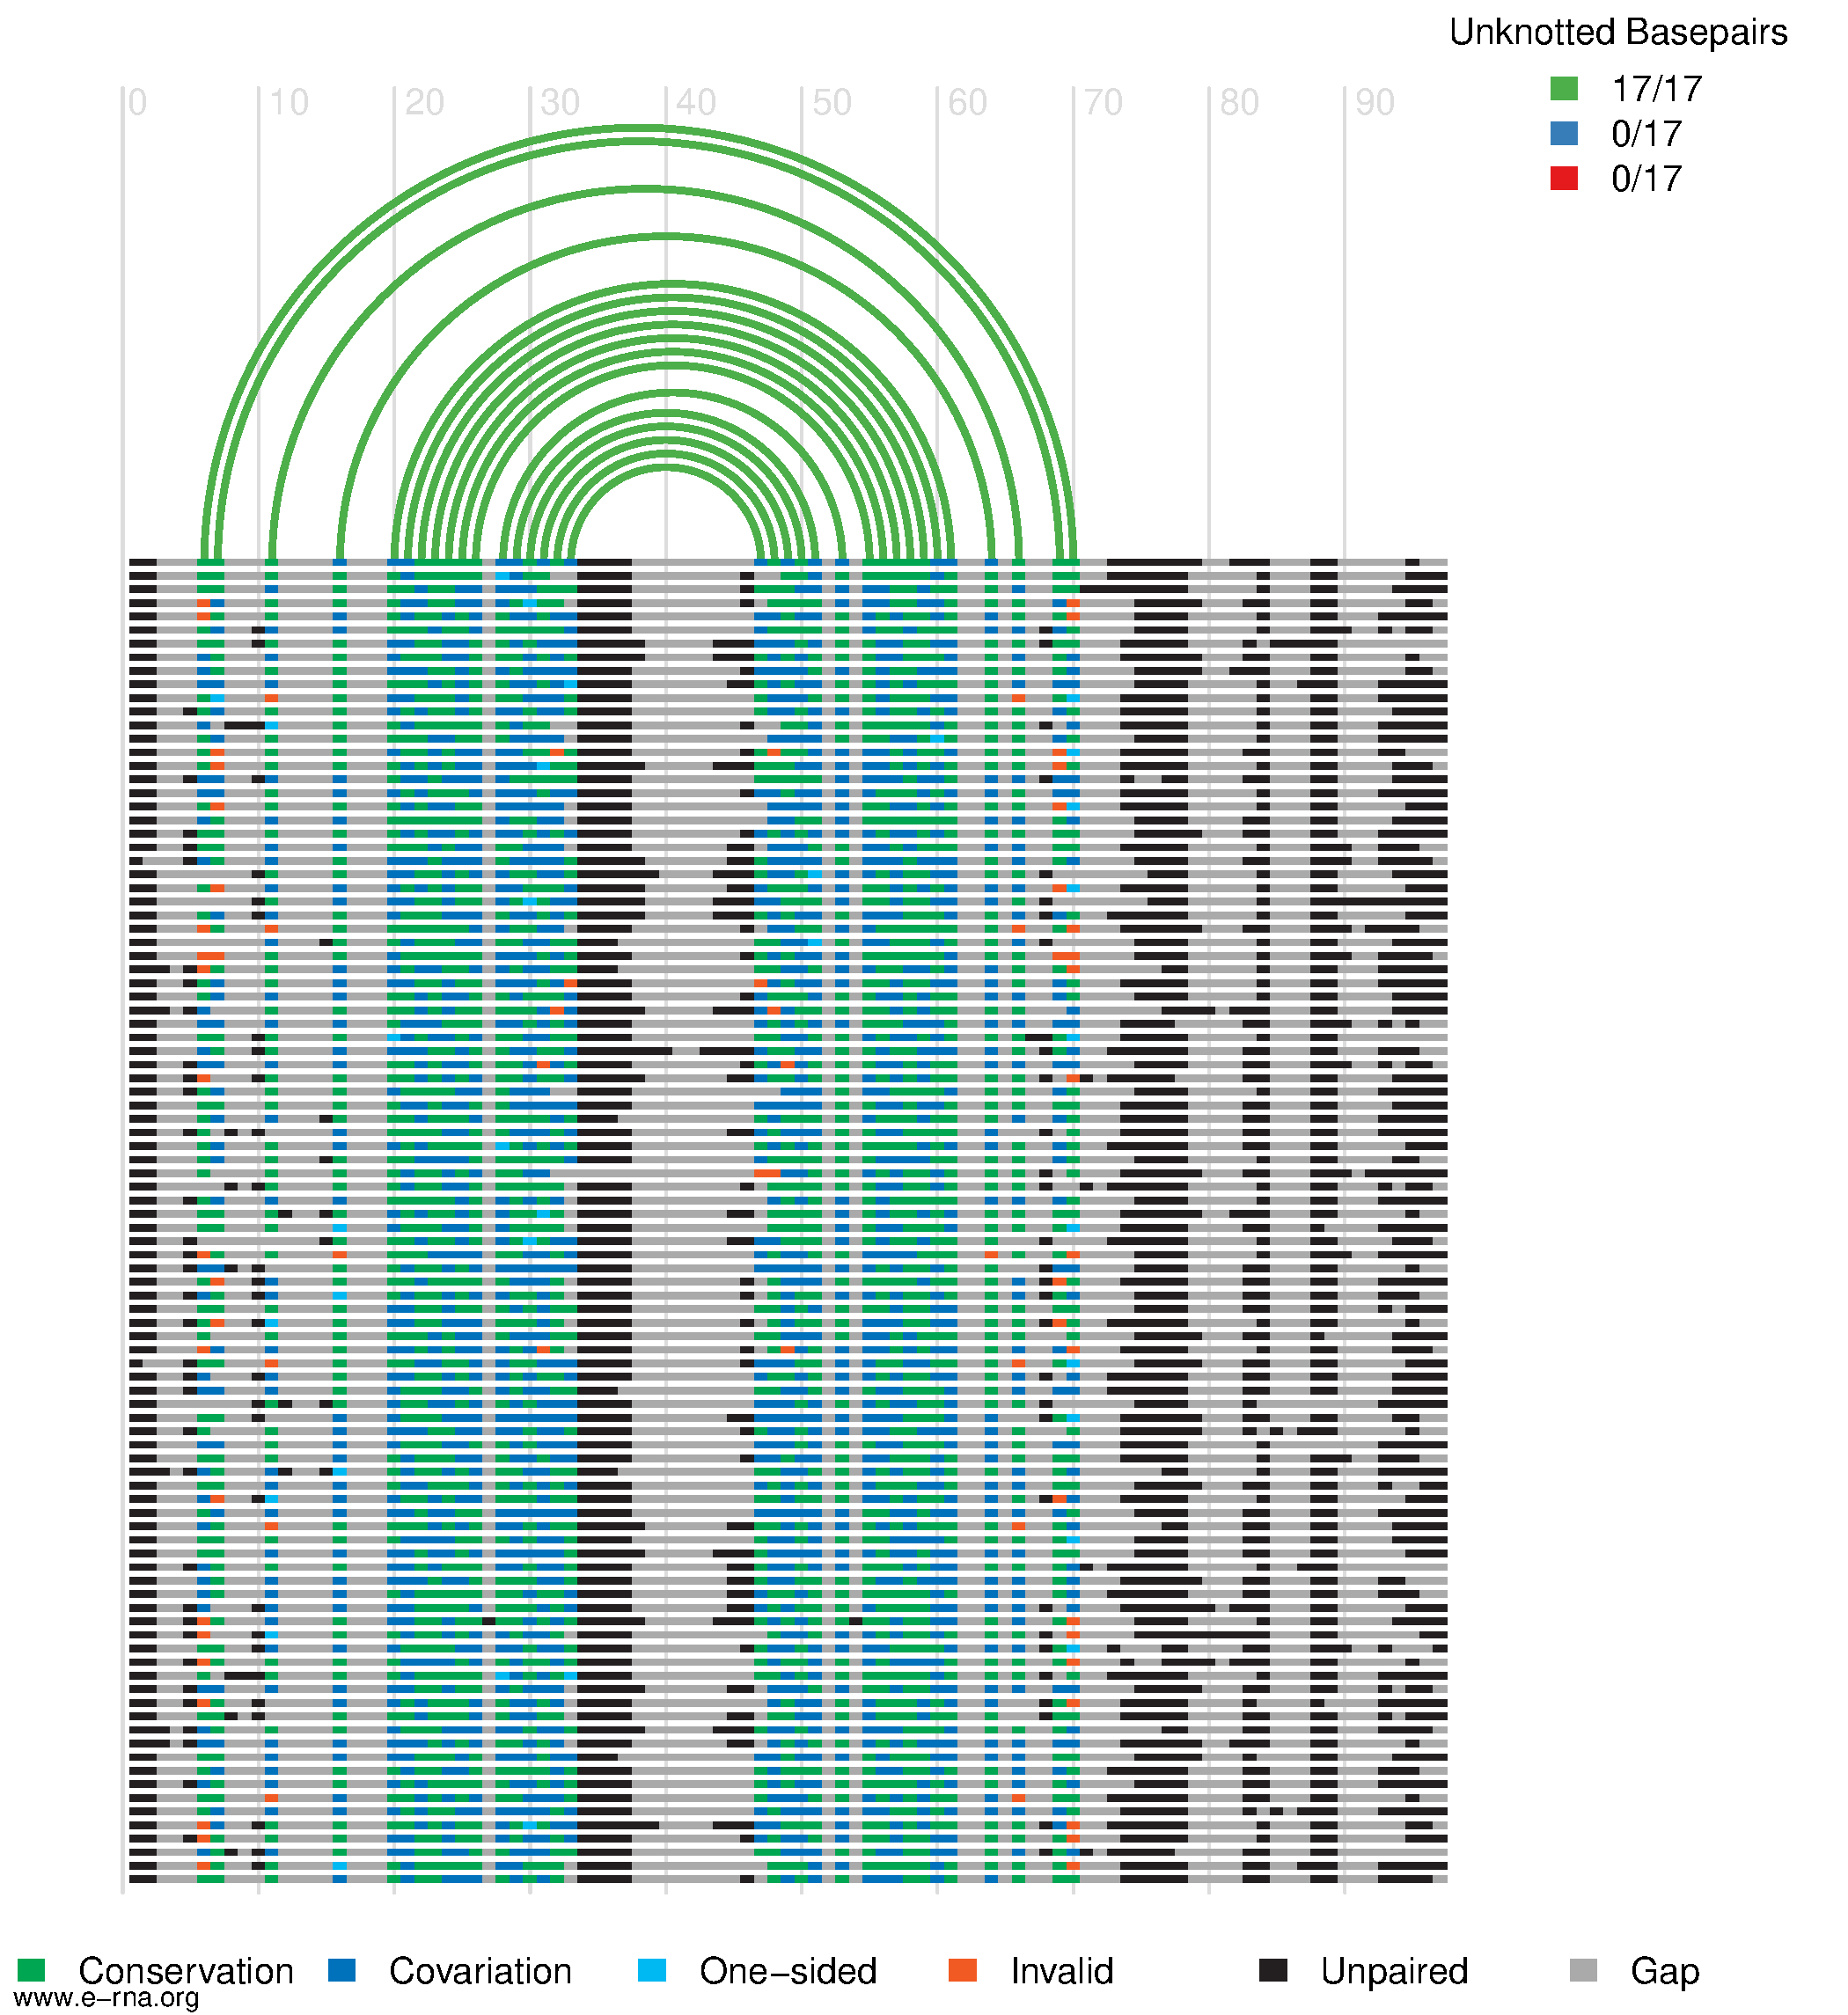
\includegraphics[width=14cm]{16_aln}
\caption[Example alignment of cluster consensus sequences]{\textbf{Example alignment of cluster consensus sequences.} Partial alignment of the consensus sequences for cluster 16, visualized using the R-CHIE webserver \parencite{Lai2012}. Green arcs represent base-pairing interactions. Nucleotides are visualized as blocks below, and are colored to highlight conservation and covariation in base-pairing relationships within the stem-loop structure.
} 
\label{fig:aln}
\end{center}
\end{figure}

I have developed a sampling based approach to measuring CM similarity. However, rather than using a single reference sequence for the purpose of comparison, I use the fact that CMs are generative models to measure the average similarity of of their respective sequence spaces. Infernal reports bitscores and E-value for each match between a CM and a given sequence region. The bitscore, ignoring the specifics of algorithm used (either CYK or Inside), is \[S = \log_2\left({\frac{P(x \mid H)}{P(x \mid R)}}\right)\] where $P(x \mid H)$ is the probability of sequence $x$ under model $H$, and $P(x \mid R)$ is the probability of $x$ under a null model $R$, generally an iid\nomenclature[Z]{iid}{Independent identically distributed (random variable)} sites model with a geometric length distribution. This score is expected to follow a Type 1 Extreme Value (or Gumbel) distribution \parencite{Karlin1990, Eddy2008}, and this empirically appears to be the case for Infernal scores \parencite{Nawrocki2007}. Hence the E-value can be calculated as \[e^{-\lambda(S - \mu)}\] where $\lambda$ and $\mu$ are fitted parameters depending on the size of the database searched and the model architecture, and normalize for these factors. So the reciprocal similarity score (RSS) I have defined: \[ RSS_{x,y} = \left[\frac{\sum_{i=1}^{n} -\ln{(E_{x,y,i})} +  \sum_{j=1}^{n} -\ln{(E_{x,y,j})}}{2n}\right] + \ln(n) \] where $E_{x,y,i}$ is the E-value of the $i$th sequence emitted by model $x$ scored by model $y$, can be understood as the average normalized bitscore of each model over the other's sequence space, and is similar in spirit to the Kullback-Leibler divergence. This measure appeared robust to the number of samples used, but this may depend in part on model complexity. As the maximal E-value in this case is $n$, $-\ln(n)$ is a theoretical lower bound on the average $-\ln{(E)}$, and the subtraction of this factor ensures that the RSS is strictly positive. It is worth noting that this measure is symmetric ignoring sampling error. Asymmetric variants may have some applications. For instance, by taking the minimum of the average bitscore under either model, one would give preference to full-length model matches in comparisons between models of various sizes due to the glocal nature of Infernal search (global with respect to the model, local with respect to sequence), and this may be preferable for determining similarity between ncRNA families. Conversely, taking the maximum may have some utility in searching for shorter motifs. In the current application, I expect all CMs to be of roughly similar sizes and symmetric measures simplify clustering. This measure should be applicable to any generative model, and so could be similarly used to cluster e.g. HMMs.

A related measure was previously used by the TRIBE-MCL algorithm to cluster protein families based on reciprocal $\log_{10}$ BLAST E-values \parencite{Enright2002}. The MCL algorithm is described in detail elsewhere \parencite{VanDongen2008}, but briefly uses simulations of random walks on a weighted graph to define clusters through an unsupervised, iterative process. Unsurprisingly, many of the clusters that were generated using MCL with RSSes appeared to be composed of CMs representing canonical RITs on visual inspection with some notable exceptions, described below. However, despite a complete lack of phylogenetic assumptions in our pipeline, we found that the majority of clusters were dominated by one or two orders, generally within the same phyla, and sometimes even a single genera. This both validates our clustering procedure and indicates that RITs, despite their small size and stereotypical composition, carry a phylogenetic signal when considered in aggregate.

To further study lineage-specific biases in terminator composition, I took the top 100 clusters, ranging in size from 332 to 6 CMs, and constructed consensus models through a semi-automated process. First, for each cluster I selected the 10 CMs with the highest sum of RSS scores with other cluster CMs (or all CMs in the case of clusters with $<$ 10 members), and searched these across all of the genomes the cluster CMs were derived from. Regions that these CMs agreed were likely to be terminator sequences were collected and aligned using MAFFT Q-INS-i \parencite{Katoh2008}, a heuristic Sankoff alignment algorithm which considers both sequence and secondary structure in alignment, and secondary structure was predicted using CentroidAlifold \parencite{Hamada2009}, and manually refined using RALEE \parencite{Griffiths-Jones2005} (see figure \ref{fig:aln}; see also Methods for detailed alignment protocol). I annotated the 1853 embl files we started with, and iteratively removed from consideration any model with at least 85\% of its sequence hits covered by another model. This left 16 putative terminator models, on which all further analysis was done.



\subsection{Lineage-specific differences in RIT utilization}

Of the 16 resulting cluster, 9 appeared to be canonical RITs on visual inspection (see figure \ref{fig:canonical}). All shared known features of canonical RITs, including a $5^\prime$ poly-A region, a G/C-rich hairpin, and a poly-U tail, but differ in stem length and base composition.

\begin{figure}[htp]
\begin{center}
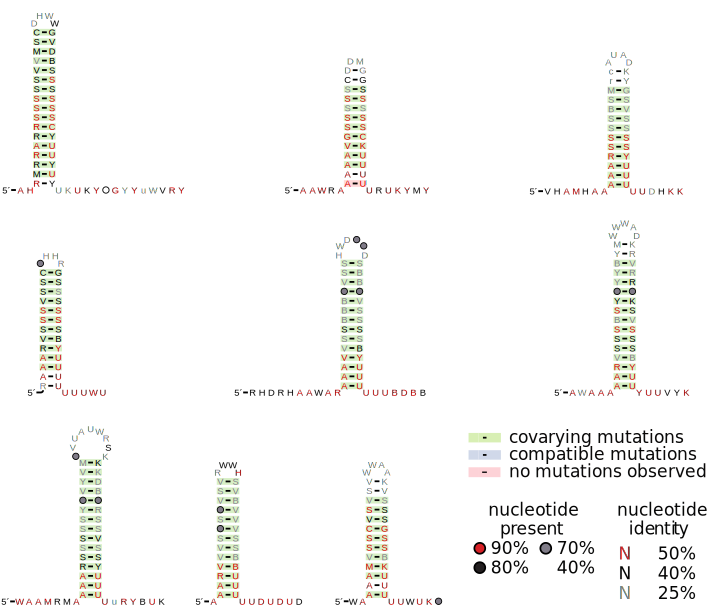
\includegraphics[width=14cm]{canonical}
\caption[Most informative sequences for nine canonical RIT clusters]{\textbf{Most informative sequence for nine canonical RIT clusters.} Each cluster consensus model was searched across all genomes and sequence hits with an FDR of 0.01 were aligned to the model. Duplicate sequences were removed and 5000 randomly sampled sequences were used to calculate the most informative sequence (MIS)\nomenclature[Z]{MIS}{Most informative sequence}, a projection of any bases with frequencies above .25 onto IUPAC characters \parencite{Freyhult2005}. Structures were drawn using R2R \parencite{Weinberg2011}. From left to right, images shown represent consensus alignments for clusters 16, 25, 29 (top row); 37, 88, 89 (middle row); 95, and 96 (bottom row).
} 
\label{fig:canonical}
\end{center}
\end{figure}

\begin{figure}[htp]
\begin{center}
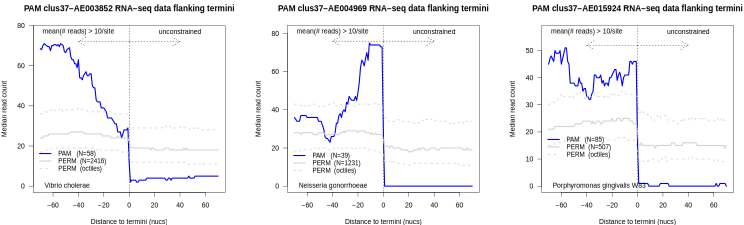
\includegraphics[width=16cm]{can_expr}
\caption[Analysis of diverse RNA-seq datasets confirm canonical terminator activity]{\textbf{Analysis of diverse RNA-seq datasets confirm canonical terminator activity.} These plots present representative analysis for putative attenuation motifs (PAM)\nomenclature[Z]{PAM}{Putative attenuation motif} by the cluster 37 canonical terminator consensus model. The median expression over PAMs with an upstream mean expression of at least 10 reads per position is plotted in blue. Random positions meeting this same constraint are plotted in grey, and the dashed grey lines provide a 75\% confidence interval for this estimate. RNA-seq data (from left to right) drawn from experiments in the $\gamma$-proteobacterium \textit{Vibrio cholerae} \parencite{Mandlik2011}, the $\beta$-proteobacterium \textit{Neisseria gonorrhoeae} \parencite{Isabella2011}, and the Bacteroidetes \textit{Porphyromonas gingivalis} \parencite{Hovik2012}.
} 
\label{fig:can_expr}
\end{center}
\end{figure}

\subsection{Non-canonical putative attenuators of transcription}

\section{Discussion}
%\include{Conclusions/conclusions}



\backmatter % book mode only
\fancyhead[LO,RE]{\textit{Published Works}}

% Thesis Published Work ---------------------------------------------------
\chapter{Publications}

Publications arising in the course of this thesis:

\itemize

\item{Read H., Johnson S., Barquist L., Mills G., Gardner P.P., Patrick W.M., Wiles S. \textbf{The effect of constitutive bioluminescence expression on the in vitro and in vivo fitness of the mouse enteropathogen \textit{Citrobacter rodentium}.} Manuscript in preparation.}

\item{Wong V., Pickard D., Barquist L., Sivaraman K., Harte P., Arends M., Kane L., Mottram L., Ellison L., Kay S., Wileman T., MacLennan, Kingsley R.A., Dougan G.  \textbf{Characterization of the yehUT two-component regulatory system of \textit{Salmonella enterica} serovars Typhi and Typhimurium}. Manuscript in preparation.}

\item{Okoro C.K., Barquist L., Kingsley R.A., Connor T.R., Harris S.R., Arends M., Stevens M., Parry C.M., Al-Mashhadani M.N., Kariuki S., Msefula C.L., Gordon M.A., de Pinna E., Wain J., Heyderman R.S., Obaro S., Alonso P.L., Mandomando I., MacLennan C.A., Tapia M.D., Levine M.M., Tennant S.M., Parkhill J., Dougan G.  \textbf{Signatures of adaptation in human invasive \textit{S.} Typhimurium populations.} Manuscript in preparation.} 

\item{Wilf N.M., Reid A.J., Ramsay J.P., Williamson N.R., Croucher N.J., Gatto L., Hester S.S., Goulding D., Barquist L., Lilley K.S., Kingsley R.A., Dougan G., Salmond G.P.C.. \textbf{RNA-seq reveals the RNA binding proteins, Hfq and RsmA, play various roles in virulence, antibiotic production and genomic flux in \textit{Serratia} sp. 39006}. Manuscript under review.}

\newpage

\item{Pettit L.J., Browne H.P., Yu L., Smits W.K., Fagan R.P., Barquist L., Martin M.J., Goulding D., Duncan S.H., Flint H.J., Dougan G., Choudhary J.S., Lawley T.D. \textbf{Functional genomics reveals that \textit{Clostridium difficile} Spo0A coordinates sproulation, virulence and metabolism.} Manuscript under review.}

\item{Reuter S., Connor T.R., Barquist L., Walker D., Feltwell T., Harris S.R., Fookes M., Hall M.E., Fuchs T.M., Corander J., Dufour M., Ringwood T., Savin C., Bouchier C., Martin L., Miettinen M., Shubin M., Laukkanen-Ninios R., Sihvonen L.M., Siitonen A., Skurnik M., Falc\~{a}o J.P., Fukushima H., Scholz H.C., Prentice M., Wren B.W., Parkhill J., Carniel E., Achtman M., McNally A., Thomson N.R. \textbf{Parallel independent evolution of pathogenicity within the genus \textit{Yersinia}.} Manuscript under review.}

\item{Barquist L., Burge S.W., Gardner P.P. \textbf{Building non-coding RNA families.} \textit{Methods in Molecular Biology}, in press.} 

\item{Hoeppner M.P., Barquist L., Gardner P.P. \textbf{An introduction to RNA databases.} \textit{Methods in Molecular Biology}, in press.} 

\item{Croucher N.J., Mitchell A.M., Gould K.A., Inverarity D., Barquist L., Feltwell T., Fookes M.C., Harris S.R., Dordel J., Salter S.J., Browall S., Zemlickova H., Parkhill J., Normark S., Henriques-Normark B., Hinds J., Mitchell T.J., Bentley S.D. \textbf{Dominant role of nucleotide substitution in the diversification of serotype 3 pneumococci over decades and during a single infection.} \textit{PLoS Genetics}, 2013.} 

\item{Kingsley R.A., Whitehead S., Connor T., Barquist L., Sait L., Holt K., Sivaraman K., Wileman T., Goulding D., Clare S., Hale C., Seshasayee A., Harris S., Thomson N., Gardner P., Rabsch W., Wigley P., Humphrey T., Parkhill J., Dougan G. \textbf{Genome and transcriptome adaptation accompanying emergence of the DT2 host-restricted \textit{Salmonella} Typhimurium pathovar.}  \textit{mBio}, 2013.}

\item{Martin M.J., Clare S., Goulding D., Faulds-Pain A., Barquist L., Browne H., Pettit L., Dougan G., Lawley T.D.,  Wren B.W. \textbf{The \textit{agr} locus regulates virulence and colonization genes in \textit{Clostridium difficile} 027.} \textit{Journal of Bacteriology}, 2013. }

\newpage

\item{Barquist L., Boinett C.J., Cain A.K..  \textbf{Approaches to querying bacterial genomes with transposon-insertion sequencing.} \textit{RNA Biology}, 10(7), 2013.}

\item{Barquist L., Langridge G.C., Turner D.J., Phan M.D., Turner A.K., Bateman A., Parkhill J., Wain J., Gardner P.P. \textbf{A comparison of dense transposon insertion libraries in the \textit{Salmonella} serovars Typhi and Typhimurium.} \textit{Nucleic Acids Research}, 41(8):4549-4564, 2013.} 

\item{Burge S.W., Daub J., Eberhardt R., Tate J., Barquist L., Nawrocki E.P., Eddy S.R., Gardner P.P., Bateman A. \textbf{Rfam 11.0: 10 years of RNA families.} \textit{Nucleic Acids Research}. 41(D1):D226-D232, 2013}

\item{Croucher N.J., Harris S.R., Barquist L., Parkhill J., Bentley S.D. \textbf{A high-resolution view of genome-wide pneumococcal transformation.} \textit{PLoS Pathogens}, 8(6), 2012}

\item{Westesson O., Barquist L., Holmes I. \textbf{HandAlign: Bayesian multiple sequence alignment, phylogeny, and ancestral reconstruction.} \textit{Bioinformatics}, 28(8):1170-1171, 2012}

\item{Gardner P.P., Barquist L., Bateman A., Nawrocki E.P., Weinberg Z. \textbf{RNIE: genome-wide prediction of bacterial intrinsic terminators.} \textit{Nucleic Acids Research}, 39(14):5845-5852, 2011}



 
 % ----------------------------------------------------------------------

%%% Local Variables: 
%%% mode: latex
%%% TeX-master: "../thesis"
%%% End: 

\fancyhead[LO,RE]{\textit{Appendix}}

\appendix
\chapter{Appendix A: Supplementary data for chapters 2 and 3}
\ifpdf
    \graphicspath{{AppendixA/AppendixAFigs/EPS/}{AppendixA/AppendixAFigs/}}
\fi

This thesis should include a CD containing supplementary data for chapters 2 and 3. This CD contains two files in Excel format.

Chapter2.xls contains the complete results of the TraDIS assays described in chapter 2, and should be identical to the supplementary information of \textcite{Barquist2013a}.

Chapter3.xls contains genomic features significantly depleted or enriched in insertions over the macrophage assays described in chapter 3.

If the CD is not enclosed, or if you are viewing this thesis electronically, contact Lars Barquist (lb14@sanger.ac.uk) to obtain these files.

% ------------------------------------------------------------------------

%%% Local Variables: 
%%% mode: latex
%%% TeX-master: "../thesis"
%%% End: 

\chapter{Appendix B: Genomic sequences analyzed for termination motifs}
\ifpdf
    \graphicspath{{AppendixB/AppendixBFigs/EPS/}{AppendixB/AppendixBFigs/}}
\fi

% Table generated by Excel2LaTeX from sheet 'TraDIS screen of Ty2 protein'
\begingroup
  \centering
     \tiny
   \noindent
  \begin{longtable}{ll}
  \caption{Genomic sequences analyzed for termination motifs in chapter 5}   
  \\ 
    \toprule
    \textbf{EMBL accession} & \textbf{Scientific name} \\
    \midrule
AP011945 & Helicobacter pylori F57\\
CP000885 & Clostridium phytofermentans ISDg\\
CP000471 & Magnetococcus marinus MC-1\\
BA000033 & Staphylococcus aureus subsp. aureus MW2\\
CP000679 & Caldicellulosiruptor saccharolyticus DSM 8903\\
CP000049 & Borrelia turicatae 91E135\\
CP002534 & Cellulophaga lytica DSM 7489\\
CP002876 & Nitrosomonas sp. Is79A3\\
AM286280 & Francisella tularensis subsp. tularensis FSC198\\
CP002505 & Rahnella sp. Y9602\\
AE016958 & Mycobacterium avium subsp. paratuberculosis K-10\\
CP000950 & Yersinia pseudotuberculosis YPIII\\
FR856862 & Novosphingobium sp. PP1Y\\
CP002819 & Ralstonia solanacearum Po82\\
FP929043 & Eubacterium rectale M104/1\\
CP002621 & Enterococcus faecalis OG1RF\\
FP929034 & Bifidobacterium longum subsp. longum F8\\
CP001150 & Rhodobacter sphaeroides KD131\\
CP002302 & Buchnera aphidicola str. JF99 (Acyrthosiphon pisum)\\
CP001158 & Buchnera aphidicola str. Tuc7 (Acyrthosiphon pisum)\\
AP012205 & Synechocystis sp. PCC 6803\\
AE015927 & Clostridium tetani E88\\
CU469464 & Candidatus Phytoplasma mali\\
CP001032 & Opitutus terrae PB90-1\\
CP002805 & Chlamydophila psittaci 01DC11\\
CP000946 & Escherichia coli ATCC 8739\\
CP000529 & Polaromonas naphthalenivorans CJ2\\
CP001071 & Akkermansia muciniphila ATCC BAA-835\\
CP001336 & Desulfitobacterium hafniense DCB-2\\
AE017126 & Prochlorococcus marinus subsp. marinus str. CCMP1375\\
CP002218 & Burkholderia sp. CCGE1003\\
BX571857 & Staphylococcus aureus subsp. aureus MSSA476\\
AP011149 & Acetobacter pasteurianus IFO 3283-26\\
AE005174 & Escherichia coli O157\\
AM422018 & Candidatus Phytoplasma australiense\\
CP001581 & Clostridium botulinum A2 str. Kyoto\\
AE017283 & Propionibacterium acnes KPA171202\\
CP002810 & Isoptericola variabilis 225\\
CP000813 & Bacillus pumilus SAFR-032\\
CP001752 & Treponema pallidum subsp. pallidum str. Chicago\\
CP000348 & Leptospira borgpetersenii serovar Hardjo-bovis str. L550\\
BX571963 & Rhodopseudomonas palustris CGA009\\
CP002811 & Shewanella baltica OS117\\
AE013598 & Xanthomonas oryzae pv. oryzae KACC 10331\\
CP002881 & Pseudomonas stutzeri ATCC 17588 = LMG 11199\\
DS180873 & Leptospirillum rubarum\\
CP002829 & Thermodesulfobacterium sp. OPB45\\
CP000606 & Shewanella loihica PV-4\\
AM902716 & Bordetella petrii\\
CP000076 & Pseudomonas protegens Pf-5\\
AP009389 & Pelotomaculum thermopropionicum SI\\
CP001037 & Nostoc punctiforme PCC 73102\\
CU468135 & Erwinia tasmaniensis Et1/99\\
CP002026 & Starkeya novella DSM 506\\
FP929051 & Ruminococcus bromii L2-63\\
CP000924 & Thermoanaerobacter pseudethanolicus ATCC 33223\\
CP000553 & Prochlorococcus marinus str. NATL1A\\
CP002728 & Tepidanaerobacter acetatoxydans Re1\\
CP002312 & Borrelia burgdorferi JD1\\
CP000384 & Mycobacterium sp. MCS\\
CP002521 & Acidovorax avenae subsp. avenae ATCC 19860\\
FN433596 & Staphylococcus aureus subsp. aureus TW20\\
CM000728 & Bacillus cereus Rock1-3\\
CR522870 & Desulfotalea psychrophila LSv54\\
CP001509 & Escherichia coli BL21(DE3)\\
AB097150 & Onion yellows phytoplasma\\
CP001960 & Campylobacter jejuni subsp. jejuni S3\\
CP000943 & Methylobacterium sp. 4-46\\
CP000667 & Salinispora tropica CNB-440\\
CP001958 & Segniliparus rotundus DSM 44985\\
CM000604 & Clostridium difficile ATCC 43255\\
CP002660 & Clostridium acetobutylicum DSM 1731\\
CP001794 & Geobacillus sp. Y412MC61\\
CP002868 & Spirochaeta caldaria DSM 7334\\
CP001959 & Brachyspira murdochii DSM 12563\\
FM242711 & Listeria monocytogenes serotype 4b str. CLIP 80459\\
FM204884 & Streptococcus equi subsp. zooepidemicus\\
CP002442 & Geobacillus sp. Y412MC52\\
CP000680 & Pseudomonas mendocina ymp\\
CP002777 & Thermus thermophilus SG0.5JP17-16\\
FN568063 & Streptococcus mitis B6\\
CP000386 & Rubrobacter xylanophilus DSM 9941\\
FR668087 & Mycoplasma leachii 99/014/6\\
AP010888 & Bifidobacterium longum subsp. longum JCM 1217\\
CP001124 & Geobacter bemidjiensis Bem\\
AM040264 & Brucella melitensis biovar Abortus 2308\\
CP001801 & Halothiobacillus neapolitanus c2\\
CP002416 & Clostridium thermocellum DSM 1313\\
CP000458 & Burkholderia cenocepacia HI2424\\
CP000828 & Acaryochloris marina MBIC11017\\
CP002890 & Escherichia coli UMNF18\\
BA000045 & Gloeobacter violaceus PCC 7421\\
AP006628 & Onion yellows phytoplasma OY-M\\
CP001981 & Candidatus Sulcia muelleri DMIN\\
CP000932 & Campylobacter lari RM2100\\
CP000774 & Parvibaculum lavamentivorans DS-1\\
CP001903 & Bacillus thuringiensis BMB171\\
CP002164 & Caldicellulosiruptor obsidiansis OB47\\
CP002825 & Lacinutrix sp. 5H-3-7-4\\
CP001196 & Oligotropha carboxidovorans OM5\\
CP000869 & Burkholderia multivorans ATCC 17616\\
AP012030 & Escherichia coli DH1\\
CP000837 & Streptococcus suis GZ1\\
CP001488 & Brucella melitensis ATCC 23457\\
CP002542 & Fluviicola taffensis DSM 16823\\
CP000685 & Flavobacterium johnsoniae UW101\\
CP001251 & Dictyoglomus turgidum DSM 6724\\
CP002767 & Shewanella baltica BA175\\
CP002334 & Helicobacter pylori Lithuania75\\
CP001184 & Ureaplasma urealyticum serovar 10 str. ATCC 33699\\
CP001930 & Chlamydia trachomatis G/9301\\
BA000008 & Chlamydophila pneumoniae J138\\
CP000803 & Francisella tularensis subsp. holarctica FTNF002-00\\
AP009484 & Macrococcus caseolyticus JCSC5402\\
CP002593 & Pseudonocardia dioxanivorans CB1190\\
CP001504 & Burkholderia glumae BGR1\\
CM000738 & Bacillus cereus AH676\\
CP000248 & Novosphingobium aromaticivorans DSM 12444\\
AE017194 & Bacillus cereus ATCC 10987\\
CP000705 & Lactobacillus reuteri DSM 20016\\
CP001281 & Thauera sp. MZ1T\\
FP236530 & Mycoplasma hominis ATCC 23114\\
CP000154 & Paenibacillus polymyxa E681\\
CP000283 & Rhodopseudomonas palustris BisB5\\
CM000776 & Helicobacter canadensis MIT 98-5491\\
AM233362 & Francisella tularensis subsp. holarctica LVS\\
CP001100 & Chloroherpeton thalassium ATCC 35110\\
AE017196 & Wolbachia endosymbiont of Drosophila melanogaster\\
BX897700 & Bartonella quintana str. Toulouse\\
CM000747 & Bacillus thuringiensis Bt407\\
CP002120 & Staphylococcus aureus subsp. aureus str. JKD6008\\
CP002627 & Bacillus amyloliquefaciens TA208\\
CP002739 & Thermoanaerobacterium xylanolyticum LX-11\\
CP002345 & Paludibacter propionicigenes WB4\\
AP012035 & Acidiphilium multivorum AIU301\\
CU234118 & Bradyrhizobium sp. ORS 278\\
CP001744 & Planctomyces limnophilus DSM 3776\\
CP000875 & Herpetosiphon aurantiacus DSM 785\\
CP002300 & Buchnera aphidicola str. LL01 (Acyrthosiphon pisum)\\
AM990992 & Staphylococcus aureus subsp. aureus ST398\\
CP001814 & Streptosporangium roseum DSM 43021\\
CP002526 & Glaciecola sp. 4H-3-7+YE-5\\
CP000910 & Renibacterium salmoninarum ATCC 33209\\
CP002927 & Bacillus amyloliquefaciens XH7\\
CP002361 & Oceanithermus profundus DSM 14977\\
CP002339 & Alteromonas sp. SN2\\
CM000661 & Clostridium difficile QCD-76w55\\
CP000108 & Chlorobium chlorochromatii CaD3\\
CP002468 & Bacillus subtilis BSn5\\
CP002096 & Helicobacter pylori 35A\\
CP002080 & Acinetobacter oleivorans DR1\\
CR628337 & Legionella pneumophila str. Lens\\
CP002124 & Erwinia sp. Ejp617\\
CP000688 & Dehalococcoides sp. BAV1\\
AE016795 & Vibrio vulnificus CMCP6\\
CP000026 & Salmonella enterica subsp. enterica serovar Paratyphi A str. ATCC 9150\\
CP000030 & Anaplasma marginale str. St. Maries\\
CP001661 & Geobacter sp. M21\\
CP001643 & Brachybacterium faecium DSM 4810\\
CP000675 & Legionella pneumophila str. Corby\\
AP008957 & Rhodococcus erythropolis PR4\\
CR354532 & Photobacterium profundum SS9\\
CM000757 & Bacillus thuringiensis serovar pulsiensis BGSC 4CC1\\
CM000748 & Bacillus thuringiensis serovar thuringiensis str. T01001\\
CP002219 & Caldicellulosiruptor hydrothermalis 108\\
CP000517 & Lactobacillus helveticus DPC 4571\\
AP010656 & Candidatus Azobacteroides pseudotrichonymphae genomovar. CFP2\\
CP002901 & Sulfobacillus acidophilus TPY\\
CP000613 & Rhodospirillum centenum SW\\
CP000115 & Nitrobacter winogradskyi Nb-255\\
BA000012 & Mesorhizobium loti MAFF303099\\
CP000048 & Borrelia hermsii DAH\\
CU459003 & Magnetospirillum gryphiswaldense MSR-1\\
CP001734 & Desulfohalobium retbaense DSM 5692\\
CP000246 & Clostridium perfringens ATCC 13124\\
CP002536 & Deinococcus proteolyticus MRP\\
AE008691 & Thermoanaerobacter tengcongensis MB4\\
AE004439 & Pasteurella multocida subsp. multocida str. Pm70\\
CP002188 & Mycoplasma bovis PG45\\
CP002185 & Escherichia coli W\\
CP000847 & Rickettsia akari str. Hartford\\
CP001598 & Bacillus anthracis str. A0248\\
CP000023 & Streptococcus thermophilus LMG 18311\\
FR773153 & Mycoplasma haemofelis str. Langford 1\\
CP002110 & Staphylococcus aureus subsp. aureus TCH60\\
CP000702 & Thermotoga petrophila RKU-1\\
AJ235269 & Rickettsia prowazekii str. Madrid E\\
CP001872 & Mycoplasma gallisepticum str. R(high)\\
CP001674 & Methylovorus glucosetrophus SIP3-4\\
AM398681 & Flavobacterium psychrophilum JIP02/86\\
CP002273 & Eubacterium limosum KIST612\\
CP001287 & Cyanothece sp. PCC 8801\\
AE008692 & Zymomonas mobilis subsp. mobilis ZM4\\
CP002516 & Escherichia coli KO11FL\\
CP001848 & Pirellula staleyi DSM 6068\\
CP000918 & Streptococcus pneumoniae 70585\\
CP001978 & Marinobacter adhaerens HP15\\
CP002616 & Lactobacillus casei LC2W\\
CP000814 & Campylobacter jejuni subsp. jejuni 81116\\
AP011540 & Rothia mucilaginosa DY-18\\
CP000247 & Escherichia coli 536\\
CP000709 & Brucella ovis ATCC 25840\\
CP001182 & Acinetobacter baumannii AB0057\\
CP002525 & Mycoplasma suis str. Illinois\\
FP929033 & Bacteroides xylanisolvens XB1A\\
CP002024 & Chlamydia trachomatis L2c\\
CP002338 & Lactobacillus amylovorus GRL 1112\\
FR775250 & Salmonella enterica subsp. enterica serovar Weltevreden str. 2007-60-3289-1\\
AP007281 & Lactobacillus reuteri JCM 1112\\
CP001322 & Desulfatibacillum alkenivorans AK-01\\
CP000821 & Shewanella sediminis HAW-EB3\\
AP012032 & Pantoea ananatis AJ13355\\
CP001234 & Vibrio cholerae M66-2\\
CP001230 & Persephonella marina EX-H1\\
CP001886 & Chlamydia trachomatis E/150\\
CP000727 & Clostridium botulinum A str. Hall\\
CM000758 & Bacillus thuringiensis IBL 200\\
FP565814 & Salinibacter ruber M8\\
FN424405 & Salmonella enterica subsp. enterica serovar Typhimurium str. D23580\\
FP929059 & Eubacterium siraeum V10Sc8a\\
CM000723 & Bacillus cereus BDRD-ST24\\
AE017340 & Idiomarina loihiensis L2TR\\
CP001348 & Clostridium cellulolyticum H10\\
CM000755 & Bacillus thuringiensis serovar pondicheriensis BGSC 4BA1\\
CP002725 & Gardnerella vaginalis HMP9231\\
CP000057 & Haemophilus influenzae 86-028NP\\
FP885895 & Ralstonia solanacearum CMR15\\
AM849034 & Clavibacter michiganensis subsp. sepedonicus\\
CP001798 & Nitrosococcus halophilus Nc4\\
BX293980 & Mycoplasma mycoides subsp. mycoides SC str. PG1\\
FM211187 & Streptococcus pneumoniae ATCC 700669\\
CP001844 & Staphylococcus aureus 04-02981\\
CU468230 & Acinetobacter baumannii\\
CM000736 & Bacillus cereus F65185\\
CP000887 & Brucella abortus S19\\
CP000395 & Borrelia afzelii PKo\\
FP929038 & Coprococcus catus GD/7\\
AE005674 & Shigella flexneri 2a str. 301\\
AP010958 & Escherichia coli O103\\
CP002171 & Thermoanaerobacterium thermosaccharolyticum DSM 571\\
CP002780 & Desulfotomaculum ruminis DSM 2154\\
CP002745 & Collimonas fungivorans Ter331\\
CP000117 & Anabaena variabilis ATCC 29413\\
CP002456 & Taylorella equigenitalis MCE9\\
CP001850 & Clostridiales genomosp. BVAB3 str. UPII9-5\\
CP002865 & Zymomonas mobilis subsp. pomaceae ATCC 29192\\
CP001736 & Kribbella flavida DSM 17836\\
CP000725 & Streptococcus gordonii str. Challis substr. CH1\\
CP002582 & Clostridium lentocellum DSM 5427\\
CP001793 & Paenibacillus sp. Y412MC10\\
CP000416 & Lactobacillus brevis ATCC 367\\
CP000036 & Shigella boydii Sb227\\
CP002857 & Corynebacterium resistens DSM 45100\\
CP000850 & Salinispora arenicola CNS-205\\
CP002910 & Klebsiella pneumoniae KCTC 2242\\
AE010300 & Leptospira interrogans serovar Lai str. 56601\\
CP001635 & Variovorax paradoxus S110\\
CP002281 & Ilyobacter polytropus DSM 2926\\
CP002634 & Bacillus amyloliquefaciens LL3\\
CP001855 & Escherichia coli O83\\
BA000004 & Bacillus halodurans C-125\\
CP000110 & Synechococcus sp. CC9605\\
CP000075 & Pseudomonas syringae pv. syringae B728a\\
CP000422 & Pediococcus pentosaceus ATCC 25745\\
CR555306 & Aromatoleum aromaticum EbN1\\
CP000031 & Ruegeria pomeroyi DSS-3\\
CP002786 & Amycolicicoccus subflavus DQS3-9A1\\
CP001633 & Francisella tularensis subsp. tularensis NE061598\\
CP001634 & Kosmotoga olearia TBF 19.5.1\\
CP000046 & Staphylococcus aureus subsp. aureus COL\\
BX470249 & Bordetella parapertussis 12822\\
CP001809 & Corynebacterium pseudotuberculosis 1002\\
CP002251 & Corynebacterium pseudotuberculosis I19\\
CP002189 & Candidatus Blochmannia vafer str. BVAF\\
BA000040 & Bradyrhizobium japonicum USDA 110\\
CP001680 & Helicobacter pylori 52\\
CP000088 & Thermobifida fusca YX\\
CP002205 & Sulfurimonas autotrophica DSM 16294\\
AP008981 & Orientia tsutsugamushi str. Ikeda\\
CT573326 & Pseudomonas entomophila L48\\
CP000114 & Streptococcus agalactiae A909\\
AL646052 & Ralstonia solanacearum GMI1000\\
FN555004 & Helicobacter mustelae 12198\\
CP001011 & Xylella fastidiosa M23\\
CM000636 & Mycobacterium kansasii ATCC 12478\\
AJ749949 & Francisella tularensis subsp. tularensis SCHU S4\\
CP001389 & Sinorhizobium fredii NGR234\\
CP000970 & Escherichia coli SMS-3-5\\
CP000359 & Deinococcus geothermalis DSM 11300\\
CP001104 & Eubacterium eligens ATCC 27750\\
BX897699 & Bartonella henselae str. Houston-1\\
CP000967 & Xanthomonas oryzae pv. oryzae PXO99A\\
CP002213 & Paenibacillus polymyxa SC2\\
CP001878 & Bacillus pseudofirmus OF4\\
CP002689 & Porphyromonas asaccharolytica DSM 20707\\
FQ312029 & Streptococcus pneumoniae INV200\\
CP001727 & Alicyclobacillus acidocaldarius subsp. acidocaldarius DSM 446\\
BX248353 & Corynebacterium diphtheriae NCTC 13129\\
FP929044 & Eubacterium siraeum 70/3\\
CP001026 & Burkholderia ambifaria MC40-6\\
AE001439 & Helicobacter pylori J99\\
CM000731 & Bacillus cereus Rock3-29\\
CP001138 & Salmonella enterica subsp. enterica serovar Agona str. SL483\\
CP000251 & Anaeromyxobacter dehalogenans 2CP-C\\
CP000853 & Alkaliphilus oremlandii OhILAs\\
CP002571 & Helicobacter pylori 2017\\
CP000316 & Polaromonas sp. JS666\\
CP001737 & Nakamurella multipartita DSM 44233\\
CP001337 & Chloroflexus aggregans DSM 9485\\
CP002121 & Streptococcus pneumoniae AP200\\
CP000749 & Marinomonas sp. MWYL1\\
CP000436 & Haemophilus somnus 129PT\\
CP002608 & Chlamydophila pecorum E58\\
CP000111 & Prochlorococcus marinus str. MIT 9312\\
CP002160 & Clostridium cellulovorans 743B\\
CP002299 & Frankia sp. EuI1c\\
CP000140 & Parabacteroides distasonis ATCC 8503\\
CP002422 & Neisseria meningitidis M01-240355\\
CP002558 & Francisella cf. novicida 3523\\
CP002162 & Micromonospora aurantiaca ATCC 27029\\
CP001837 & Staphylococcus lugdunensis HKU09-01\\
U00096 & Escherichia coli str. K-12 substr. MG1655\\
CP002336 & Helicobacter pylori SouthAfrica7\\
CP001145 & Coprothermobacter proteolyticus DSM 5265\\
CP000777 & Leptospira biflexa serovar Patoc strain 'Patoc 1 (Ames)'\\
CP000360 & Candidatus Koribacter versatilis Ellin345\\
AE016877 & Bacillus cereus ATCC 14579\\
CP001562 & Bartonella grahamii as4aup\\
AM920689 & Xanthomonas campestris pv. campestris\\
FR872580 & Parachlamydia acanthamoebae UV-7\\
AP010968 & Kitasatospora setae KM-6054\\
CP001797 & Pseudoalteromonas sp. SM9913\\
CP000969 & Thermotoga sp. RQ2\\
CP001843 & Treponema primitia ZAS-2\\
CP001656 & Paenibacillus sp. JDR-2\\
CP000720 & Yersinia pseudotuberculosis IP 31758\\
CP001820 & Veillonella parvula DSM 2008\\
CP001759 & Anaplasma centrale str. Israel\\
AE007317 & Streptococcus pneumoniae R6\\
BX072543 & Tropheryma whipplei TW08/27\\
BX548174 & Prochlorococcus marinus subsp. pastoris str. CCMP1986\\
FN806773 & Propionibacterium freudenreichii subsp. shermanii CIRM-BIA1\\
CP001841 & Treponema azotonutricium ZAS-9\\
CP002419 & Neisseria meningitidis G2136\\
CP001769 & Spirosoma linguale DSM 74\\
CP000681 & Shewanella putrefaciens CN-32\\
CP001191 & Rhizobium leguminosarum bv. trifolii WSM2304\\
AE000511 & Helicobacter pylori 26695\\
AE015924 & Porphyromonas gingivalis W83\\
CP002159 & Gallionella capsiferriformans ES-2\\
CP001217 & Helicobacter pylori P12\\
CP002409 & Propionibacterium acnes 266\\
AP012203 & Porphyromonas gingivalis TDC60\\
CP002167 & Escherichia coli UM146\\
FN667741 & Xenorhabdus bovienii SS-2004\\
CM000744 & Bacillus mycoides Rock3-17\\
CP002669 & Mycoplasma hyorhinis MCLD\\
CM000913 & Streptomyces clavuligerus ATCC 27064\\
CP000109 & Thiomicrospira crunogena XCL-2\\
CM000724 & Bacillus cereus BDRD-ST26\\
CP001291 & Cyanothece sp. PCC 7424\\
CM000714 & Bacillus cereus m1293\\
CP000975 & Methylacidiphilum infernorum V4\\
CP001867 & Geodermatophilus obscurus DSM 43160\\
AE002160 & Chlamydia muridarum Nigg\\
CP002158 & Fibrobacter succinogenes subsp. succinogenes S85\\
CP000096 & Chlorobium luteolum DSM 273\\
CP001931 & Thermocrinis albus DSM 14484\\
AE017334 & Bacillus anthracis str. 'Ames Ancestor'\\
CP001650 & Zunongwangia profunda SM-A87\\
CP000578 & Rhodobacter sphaeroides ATCC 17029\\
CP000634 & Agrobacterium vitis S4\\
AP008232 & Sodalis glossinidius str. 'morsitans'\\
AM889285 & Gluconacetobacter diazotrophicus PAl 5\\
FQ859185 & Streptomyces cattleya NRRL 8057 = DSM 46488\\
BA000035 & Corynebacterium efficiens YS-314\\
AP011142 & Acetobacter pasteurianus IFO 3283-22\\
AP011941 & Helicobacter pylori F30\\
AP011135 & Acetobacter pasteurianus IFO 3283-07\\
CP001407 & Bacillus cereus 03BB102\\
CP000090 & Ralstonia eutropha JMP134\\
CP000419 & Streptococcus thermophilus LMD-9\\
CP002086 & Nitrosococcus watsonii C-113\\
CP002439 & Staphylococcus pseudintermedius HKU10-03\\
AE016825 & Chromobacterium violaceum ATCC 12472\\
FP929036 & Butyrivibrio fibrisolvens 16/4\\
CP000253 & Staphylococcus aureus subsp. aureus NCTC 8325\\
AE016822 & Leifsonia xyli subsp. xyli str. CTCB07\\
CP000095 & Prochlorococcus marinus str. NATL2A\\
CP001044 & Burkholderia phymatum STM815\\
AE017333 & Bacillus licheniformis DSM 13 = ATCC 14580\\
AP010655 & Streptococcus mutans NN2025\\
CM000718 & Bacillus cereus MM3\\
CP001034 & Natranaerobius thermophilus JW/NM-WN-LF\\
AE000512 & Thermotoga maritima MSB8\\
CP001022 & Exiguobacterium sibiricum 255-15\\
FM864216 & Mycoplasma conjunctivae\\
CP000563 & Shewanella baltica OS155\\
CP002085 & Desulfarculus baarsii DSM 2075\\
CM000720 & Bacillus cereus R309803\\
CP001940 & Desulfurivibrio alkaliphilus AHT2\\
CP001928 & Waddlia chondrophila WSU 86-1044\\
CP002222 & Lactobacillus plantarum subsp. plantarum ST-III\\
CP001792 & Fibrobacter succinogenes subsp. succinogenes S85\\
CP002170 & Mycoplasma hyorhinis HUB-1\\
CP000409 & Rickettsia canadensis str. McKiel\\
FN434113 & Erwinia amylovora CFBP1430\\
AP009380 & Porphyromonas gingivalis ATCC 33277\\
CP000819 & Escherichia coli B str. REL606\\
CP001707 & Kangiella koreensis DSM 16069\\
FP929140 & gamma proteobacterium HdN1\\
CP001277 & Candidatus Hamiltonella defensa 5AT (Acyrthosiphon pisum)\\
AP012027 & Erysipelothrix rhusiopathiae str. Fujisawa\\
AE017332 & Mycoplasma hyopneumoniae 232\\
AP008971 & Finegoldia magna ATCC 29328\\
CP000437 & Francisella tularensis subsp. holarctica OSU18\\
CP002605 & Helicobacter pylori 83\\
CP000388 & Pseudoalteromonas atlantica T6c\\
CP002657 & Alicycliphilus denitrificans K601\\
CU928160 & Escherichia coli IAI1\\
CP002869 & Paenibacillus mucilaginosus KNP414\\
AP012200 & Melissococcus plutonius ATCC 35311\\
FP929040 & Enterobacter cloacae subsp. cloacae NCTC 9394\\
CP001617 & Lactobacillus plantarum JDM1\\
CP001738 & Thermomonospora curvata DSM 43183\\
CP000859 & Desulfococcus oleovorans Hxd3\\
CP000569 & Actinobacillus pleuropneumoniae serovar 5b str. L20\\
CP001996 & Staphylococcus aureus subsp. aureus ED133\\
FM872307 & Chlamydia trachomatis B/TZ1A828/OT\\
BA000034 & Streptococcus pyogenes SSI-1\\
FM252032 & Streptococcus suis BM407\\
CP002047 & Streptomyces bingchenggensis BCW-1\\
CP002130 & Candidatus Midichloria mitochondrii IricVA\\
FN392235 & Erwinia pyrifoliae DSM 12163\\
CP000025 & Campylobacter jejuni RM1221\\
AP011943 & Helicobacter pylori F32\\
CP001279 & Nautilia profundicola AmH\\
CP002794 & Bifidobacterium longum subsp. longum KACC 91563\\
CP000236 & Ehrlichia chaffeensis str. Arkansas\\
CP001995 & Mycoplasma fermentans JER\\
CM000487 & Bacillus subtilis subsp. subtilis str. 168\\
AP011548 & Lactobacillus rhamnosus GG\\
CP002183 & Bacillus subtilis subsp. spizizenii str. W23\\
AE015451 & Pseudomonas putida KT2440\\
CP002400 & Ethanoligenens harbinense YUAN-3\\
CM000726 & Bacillus cereus BDRD-Cer4\\
AP006840 & Symbiobacterium thermophilum IAM 14863\\
CP000948 & Escherichia coli str. K-12 substr. DH10B\\
AP009493 & Streptomyces griseus subsp. griseus NBRC 13350\\
FQ312030 & Streptococcus pneumoniae INV104\\
CP000393 & Trichodesmium erythraeum IMS101\\
CP000302 & Shewanella denitrificans OS217\\
CP001391 & Wolbachia sp. wRi\\
FP929053 & Ruminococcus sp. SR1/5\\
CP002341 & Lactobacillus delbrueckii subsp. bulgaricus ND02\\
CP002271 & Stigmatella aurantiaca DW4/3-1\\
CP001778 & Stackebrandtia nassauensis DSM 44728\\
CM000789 & Mycobacterium tuberculosis KZN R506\\
CP000264 & Jannaschia sp. CCS1\\
CP001607 & Aggregatibacter aphrophilus NJ8700\\
CP002331 & Helicobacter pylori India7\\
CP002528 & Krokinobacter sp. 4H-3-7-5\\
CM000737 & Bacillus cereus AH603\\
CP001638 & Geobacillus sp. WCH70\\
CP002198 & Cyanothece sp. PCC 7822\\
CP000382 & Clostridium novyi NT\\
CP002006 & Prevotella ruminicola 23\\
CP000301 & Rhodopseudomonas palustris BisB18\\
CP001487 & Blattabacterium sp. (Blattella germanica) str. Bge\\
CP001605 & Candidatus Sulcia muelleri SMDSEM\\
CP000051 & Chlamydia trachomatis A/HAR-13\\
CP002034 & Lactobacillus salivarius CECT 5713\\
CP001364 & Chloroflexus sp. Y-400-fl\\
CP000097 & Synechococcus sp. CC9902\\
BA000018 & Staphylococcus aureus subsp. aureus N315\\
CP000962 & Clostridium botulinum A3 str. Loch Maree\\
AM406671 & Lactococcus lactis subsp. cremoris MG1363\\
CP002458 & Mycoplasma fermentans M64\\
CP002614 & Salmonella enterica subsp. enterica serovar Typhimurium str. UK-1\\
CP000546 & Burkholderia mallei NCTC 10229\\
AE002098 & Neisseria meningitidis MC58\\
CP002552 & Nitrosomonas sp. AL212\\
CP002824 & Enterobacter aerogenes KCTC 2190\\
L42023 & Haemophilus influenzae Rd KW20\\
CP002390 & Filifactor alocis ATCC 35896\\
CP001213 & Bifidobacterium animalis subsp. lactis AD011\\
CP000926 & Pseudomonas putida GB-1\\
CP002028 & Thermincola potens JR\\
CP002330 & Caldicellulosiruptor kronotskyensis 2002\\
CP001853 & Bifidobacterium animalis subsp. lactis BB-12\\
CP001585 & Yersinia pestis D106004\\
FN543502 & Citrobacter rodentium ICC168\\
CP000804 & Roseiflexus castenholzii DSM 13941\\
CP000512 & Acidovorax citrulli AAC00-1\\
CP001791 & Bacillus selenitireducens MLS10\\
CP001672 & Methylotenera mobilis JLW8\\
CP002797 & Escherichia coli NA114\\
CP001252 & Shewanella baltica OS223\\
CP001321 & Haemophilus parasuis SH0165\\
CP001684 & Slackia heliotrinireducens DSM 20476\\
CP000576 & Prochlorococcus marinus str. MIT 9301\\
FP929049 & Roseburia intestinalis M50/1\\
CP001069 & Ralstonia pickettii 12J\\
FP929061 & butyrate-producing bacterium SSC/2\\
FQ312003 & Salmonella enterica subsp. enterica serovar Typhimurium str. SL1344\\
FQ312005 & Bacteriovorax marinus SJ\\
FQ312027 & Streptococcus pneumoniae OXC141\\
AM167904 & Bordetella avium 197N\\
CP000644 & Aeromonas salmonicida subsp. salmonicida A449\\
CP001962 & Thermus scotoductus SA-01\\
CR931997 & Corynebacterium jeikeium K411\\
CP002816 & Listeria monocytogenes M7\\
CP001097 & Chlorobium limicola DSM 245\\
CP001157 & Azotobacter vinelandii DJ\\
CP001033 & Streptococcus pneumoniae CGSP14\\
BA000043 & Geobacillus kaustophilus HTA426\\
CP001020 & Coxiella burnetii CbuK_Q154\\
FN668944 & Clostridium difficile BI9\\
CP000750 & Kineococcus radiotolerans SRS30216\\
CP001197 & Desulfovibrio vulgaris str. 'Miyazaki F'\\
CP000412 & Lactobacillus delbrueckii subsp. bulgaricus ATCC BAA-365\\
CP000942 & Ureaplasma parvum serovar 3 str. ATCC 27815\\
FP236842 & Erwinia pyrifoliae Ep1/96\\
CP000252 & Syntrophus aciditrophicus SB\\
BA000036 & Corynebacterium glutamicum ATCC 13032\\
CM000735 & Bacillus cereus Rock4-18\\
CP002293 & Geobacillus sp. Y4.1MC1\\
CP000951 & Synechococcus sp. PCC 7002\\
CP002465 & Streptococcus suis JS14\\
CU179680 & Mycoplasma agalactiae PG2\\
CP001900 & Campylobacter jejuni subsp. jejuni M1\\
BX950851 & Pectobacterium atrosepticum SCRI1043\\
CP000524 & Bartonella bacilliformis KC583\\
CP001873 & Mycoplasma gallisepticum str. F\\
CP000449 & Maricaulis maris MCS10\\
FP929052 & Ruminococcus champanellensis 18P13\\
CM000729 & Bacillus cereus Rock1-15\\
CP002154 & Edwardsiella tarda FL6-60\\
CP000930 & Heliobacterium modesticaldum Ice1\\
CP002917 & Corynebacterium variabile DSM 44702\\
CP002924 & Corynebacterium pseudotuberculosis PAT10\\
CP001298 & Methylobacterium chloromethanicum CM4\\
FM200053 & Salmonella enterica subsp. enterica serovar Paratyphi A str. AKU_12601\\
AP009510 & uncultured Termite group 1 bacterium phylotype Rs-D17\\
AE017308 & Mycoplasma mobile 163K\\
CP002623 & Roseobacter litoralis Och 149\\
BA000021 & Wigglesworthia glossinidia endosymbiont of Glossina brevipalpis\\
CP001604 & Listeria monocytogenes 08-5923\\
FP929062 & butyrate-producing bacterium SS3/4\\
CP000770 & Candidatus Sulcia muelleri GWSS\\
CP000890 & Coxiella burnetii RSA 331\\
CP002025 & Brachyspira pilosicoli 95/1000\\
CP002543 & Desulfurobacterium thermolithotrophum DSM 11699\\
CP001133 & Vibrio fischeri MJ11\\
CP001628 & Micrococcus luteus NCTC 2665\\
CP001631 & Acidimicrobium ferrooxidans DSM 10331\\
CP000653 & Enterobacter sp. 638\\
FP929056 & Synergistetes bacterium SGP1\\
FN665653 & Clostridium difficile M120\\
CP000413 & Lactobacillus gasseri ATCC 33323\\
CR925677 & Ehrlichia ruminantium str. Gardel\\
FR878060 & Mycobacterium africanum GM041182\\
AE017243 & Mycoplasma hyopneumoniae J\\
CP002277 & Haemophilus influenzae R2866\\
CP000488 & Candidatus Ruthia magnifica str. Cm (Calyptogena magnifica)\\
AP008230 & Desulfitobacterium hafniense Y51\\
CP000769 & Anaeromyxobacter sp. Fw109-5\\
CP001146 & Dictyoglomus thermophilum H-6-12\\
CP000721 & Clostridium beijerinckii NCIMB 8052\\
AP009152 & Kocuria rhizophila DC2201\\
CP002224 & Ketogulonicigenium vulgare Y25\\
AE017354 & Legionella pneumophila subsp. pneumophila str. Philadelphia 1\\
CP000931 & Shewanella halifaxensis HAW-EB4\\
BX571966 & Burkholderia pseudomallei K96243\\
CP000473 & Candidatus Solibacter usitatus Ellin6076\\
FR877557 & Salmonella bongori NCTC 12419\\
CP001486 & Vibrio cholerae MJ-1236\\
AP009384 & Azorhizobium caulinodans ORS 571\\
FQ312044 & Streptococcus pneumoniae SPN994039\\
CP001220 & Comamonas testosteroni CNB-2\\
CP001905 & Thioalkalivibrio sp. K90mix\\
CP002804 & Chlamydophila psittaci C19/98\\
FQ790233 & Mycoplasma suis KI3806\\
CP002280 & Rothia dentocariosa ATCC 17931\\
CP002097 & Corynebacterium pseudotuberculosis FRC41\\
CP000703 & Staphylococcus aureus subsp. aureus JH9\\
CP002478 & Staphylococcus pseudintermedius ED99\\
CP002743 & Bifidobacterium breve ACS-071-V-Sch8b\\
CP002077 & Mycoplasma pneumoniae FH\\
CP002346 & Riemerella anatipestifer ATCC 11845 = DSM 15868\\
CP000285 & Chromohalobacter salexigens DSM 3043\\
CU466930 & Candidatus Cloacamonas acidaminovorans str. Evry\\
CP000016 & Candidatus Blochmannia pennsylvanicus str. BPEN\\
CU458896 & Mycobacterium abscessus\\
CP000717 & Mycobacterium tuberculosis F11\\
CP002054 & Chlamydia trachomatis D-LC\\
CP002549 & Chlamydophila psittaci 6BC\\
CP001739 & Sebaldella termitidis ATCC 33386\\
CP001612 & Rickettsia africae ESF-5\\
CP000239 & Synechococcus sp. JA-3-3Ab\\
CP002421 & Neisseria meningitidis M01-240149\\
AE009440 & Chlamydophila pneumoniae TW-183\\
CP001666 & Clostridium ljungdahlii DSM 13528\\
CP001013 & Leptothrix cholodnii SP-6\\
CP001275 & Thermomicrobium roseum DSM 5159\\
CP000487 & Campylobacter fetus subsp. fetus 82-40\\
CP000144 & Rhodobacter sphaeroides 2.4.1\\
CP000949 & Pseudomonas putida W619\\
CP001746 & Bacillus cereus biovar anthracis str. CI\\
CP000555 & Methylibium petroleiphilum PM1\\
AL111168 & Campylobacter jejuni subsp. jejuni NCTC 11168 = ATCC 700819\\
CP002011 & Clostridium botulinum F str. 230613\\
CP001175 & Listeria monocytogenes HCC23\\
FN666575 & Erwinia amylovora ATCC 49946\\
CP000158 & Hyphomonas neptunium ATCC 15444\\
CP001619 & Dyadobacter fermentans DSM 18053\\
CP002104 & Gardnerella vaginalis ATCC 14019\\
CP000730 & Staphylococcus aureus subsp. aureus USA300_TCH1516\\
CP001677 & Candidatus Liberibacter asiaticus str. psy62\\
CP001215 & Bacillus anthracis str. CDC 684\\
CP000245 & Ramlibacter tataouinensis TTB310\\
FP475956 & Thiomonas sp. 3As\\
CP000482 & Pelobacter propionicus DSM 2379\\
CP001185 & Thermosipho africanus TCF52B\\
CP000671 & Haemophilus influenzae PittEE\\
CP000849 & Rickettsia bellii OSU 85-389\\
FR873482 & Streptococcus salivarius JIM8777\\
AP011156 & Acetobacter pasteurianus IFO 3283-32\\
CM000439 & Burkholderia thailandensis E264\\
CP000024 & Streptococcus thermophilus CNRZ1066\\
CP000394 & Granulibacter bethesdensis CGDNIH1\\
CP002216 & Caldicellulosiruptor owensensis OL\\
CP002522 & Acinetobacter baumannii TCDC-AB0715\\
FP103042 & Methylobacterium extorquens DM4\\
CP002630 & Marinithermus hydrothermalis DSM 14884\\
CP002466 & Thermoanaerobacter brockii subsp. finnii Ako-1\\
CM000770 & Rickettsia endosymbiont of Ixodes scapularis\\
AP009387 & Burkholderia multivorans ATCC 17616\\
AP006841 & Bacteroides fragilis YCH46\\
CP001819 & Sanguibacter keddieii DSM 10542\\
CP000438 & Pseudomonas aeruginosa UCBPP-PA14\\
CP002773 & Serratia plymuthica AS9\\
CP001144 & Salmonella enterica subsp. enterica serovar Dublin str. CT_02021853\\
DQ489736 & Leuconostoc citreum KM20\\
CP002113 & Capnocytophaga canimorsus Cc5\\
CP002033 & Lactobacillus fermentum CECT 5716\\
AE013218 & Buchnera aphidicola str. Sg (Schizaphis graminum)\\
CP000312 & Clostridium perfringens SM101\\
CM000743 & Bacillus mycoides Rock1-4\\
FP929039 & Coprococcus sp. ART55/1\\
CP001983 & Bacillus megaterium QM B1551\\
AE004969 & Neisseria gonorrhoeae FA 1090\\
CP000233 & Lactobacillus salivarius UCC118\\
CP002455 & Weeksella virosa DSM 16922\\
AE016853 & Pseudomonas syringae pv. tomato str. DC3000\\
AE017042 & Yersinia pestis biovar Microtus str. 91001\\
CP002459 & Brucella melitensis M28\\
CP000448 & Syntrophomonas wolfei subsp. wolfei str. Goettingen\\
CP002764 & Lactobacillus kefiranofaciens ZW3\\
CP002326 & Caldicellulosiruptor kristjanssonii 177R1B\\
CP002279 & Mesorhizobium opportunistum WSM2075\\
CP002371 & Candidatus Liberibacter solanacearum CLso-ZC1\\
AE017143 & Haemophilus ducreyi 35000HP\\
CP000612 & Desulfotomaculum reducens MI-1\\
CP000012 & Helicobacter pylori 51\\
CP001921 & Acinetobacter baumannii 1656-2\\
CP001854 & Conexibacter woesei DSM 14684\\
CP000884 & Delftia acidovorans SPH-1\\
CP002052 & Chlamydia trachomatis D-EC\\
CP000381 & Neisseria meningitidis 053442\\
CP002083 & Hyphomicrobium denitrificans ATCC 51888\\
CP002329 & Mycobacterium sp. JDM601\\
BX470251 & Photorhabdus luminescens subsp. laumondii TTO1\\
AM494475 & Orientia tsutsugamushi str. Boryong\\
AE003852 & Vibrio cholerae O1 biovar El Tor str. N16961\\
CP001589 & Yersinia pestis D182038\\
CP000759 & Ochrobactrum anthropi ATCC 49188\\
CP001968 & Denitrovibrio acetiphilus DSM 12809\\
CM000741 & Bacillus cereus AH1273\\
CP000001 & Bacillus cereus E33L\\
CP000383 & Cytophaga hutchinsonii ATCC 33406\\
CP000441 & Burkholderia ambifaria AMMD\\
BX548020 & Synechococcus sp. WH 8102\\
CR954247 & Pseudoalteromonas haloplanktis TAC125\\
CP000107 & Ehrlichia canis str. Jake\\
CP001132 & Acidithiobacillus ferrooxidans ATCC 53993\\
BA000026 & Mycoplasma penetrans HF-2\\
CP001063 & Shigella boydii CDC 3083-94\\
BX936398 & Yersinia pseudotuberculosis IP 32953\\
AP010904 & Desulfovibrio magneticus RS-1\\
CP002643 & Staphylococcus aureus subsp. aureus T0131\\
CM000750 & Bacillus thuringiensis serovar pakistani str. T13001\\
CP001339 & Thioalkalivibrio sulfidophilus HL-EbGr7\\
CP001091 & Actinobacillus pleuropneumoniae serovar 7 str. AP76\\
CP000786 & Leptospira biflexa serovar Patoc strain 'Patoc 1 (Paris)'\\
CM000732 & Bacillus cereus Rock3-42\\
AE017282 & Methylococcus capsulatus str. Bath\\
CP000661 & Rhodobacter sphaeroides ATCC 17025\\
CP001561 & Neisseria meningitidis alpha710\\
CP001621 & Mycoplasma mycoides subsp. capri str. GM12\\
CP002286 & Bifidobacterium longum subsp. longum BBMN68\\
CP000716 & Thermosipho melanesiensis BI429\\
CP000414 & Leuconostoc mesenteroides subsp. mesenteroides ATCC 8293\\
CM000753 & Bacillus thuringiensis serovar berliner ATCC 10792\\
AM260479 & Ralstonia eutropha H16\\
FP929050 & Roseburia intestinalis XB6B4\\
CP001129 & Streptococcus equi subsp. zooepidemicus MGCS10565\\
CP002039 & Herbaspirillum seropedicae SmR1\\
CP001678 & Hirschia baltica ATCC 49814\\
CP001720 & Desulfotomaculum acetoxidans DSM 771\\
CU914168 & Ralstonia solanacearum IPO1609\\
CP001080 & Sulfurihydrogenibium sp. YO3AOP1\\
CP002618 & Lactobacillus casei BD-II\\
FR873481 & Streptococcus salivarius CCHSS3\\
CP002399 & Micromonospora sp. L5\\
CP001052 & Burkholderia phytofirmans PsJN\\
CP001811 & Butyrivibrio proteoclasticus B316\\
AP010889 & Bifidobacterium longum subsp. infantis ATCC 15697 = JCM 1222\\
CP000544 & Halorhodospira halophila SL1\\
CP001078 & Clostridium botulinum E3 str. Alaska E43\\
CP002050 & Geobacillus sp. C56-T3\\
AE017223 & Brucella abortus bv. 1 str. 9-941\\
CP001511 & Methylobacterium extorquens AM1\\
CP001632 & Capnocytophaga ochracea DSM 7271\\
CP000611 & Mycobacterium tuberculosis H37Ra\\
FM177140 & Lactobacillus casei BL23\\
AE017197 & Rickettsia typhi str. Wilmington\\
CP000923 & Thermoanaerobacter sp. X514\\
CP002165 & Xylella fastidiosa subsp. fastidiosa GB514\\
AM260522 & Helicobacter acinonychis str. Sheeba\\
CP000230 & Rhodospirillum rubrum ATCC 11170\\
FM999788 & Neisseria meningitidis 8013\\
BX470248 & Bordetella pertussis Tohama I\\
CP000444 & Shewanella sp. MR-7\\
CP000492 & Chlorobium phaeobacteroides DSM 266\\
AE004091 & Pseudomonas aeruginosa PAO1\\
CP001685 & Leptotrichia buccalis C-1013-b\\
CP001472 & Acidobacterium capsulatum ATCC 51196\\
CP000490 & Paracoccus denitrificans PD1222\\
CP000857 & Salmonella enterica subsp. enterica serovar Paratyphi C strain RKS4594\\
CP001965 & Sideroxydans lithotrophicus ES-1\\
CP000672 & Haemophilus influenzae PittGG\\
CP000156 & Lactobacillus delbrueckii subsp. bulgaricus 2038\\
CP001807 & Rhodothermus marinus DSM 4252\\
CU207366 & Gramella forsetii KT0803\\
CP000259 & Streptococcus pyogenes MGAS9429\\
CP000410 & Streptococcus pneumoniae D39\\
CP001084 & Lactobacillus casei str. Zhang\\
FN563149 & Rhodococcus equi 103S\\
CP001649 & Desulfovibrio salexigens DSM 2638\\
CP001671 & Escherichia coli ABU 83972\\
CP001907 & Bacillus thuringiensis serovar chinensis CT-43\\
CP002870 & Pseudomonas putida S16\\
CP000915 & Francisella tularensis subsp. mediasiatica FSC147\\
CP001829 & Corynebacterium pseudotuberculosis C231\\
AE014299 & Shewanella oneidensis MR-1\\
AE016827 & Mannheimia succiniciproducens MBEL55E\\
CP002637 & Selenomonas sputigena ATCC 35185\\
CP000325 & Mycobacterium ulcerans Agy99\\
AP007255 & Magnetospirillum magneticum AMB-1\\
CP001408 & Burkholderia pseudomallei MSHR346\\
CP002620 & Pseudomonas mendocina NK-01\\
AM711867 & Clavibacter michiganensis subsp. michiganensis NCPPB 382\\
CP000385 & Mycobacterium sp. MCS\\
CP002156 & Parvularcula bermudensis HTCC2503\\
CM000441 & Clostridium difficile QCD-66c26\\
CP000683 & Rickettsia massiliae MTU5\\
CP001085 & Candidatus Riesia pediculicola USDA\\
BX470250 & Bordetella bronchiseptica RB50\\
CP002355 & Sulfuricurvum kujiense DSM 16994\\
CP002899 & Weissella koreensis KACC 15510\\
CP000157 & Erythrobacter litoralis HTCC2594\\
CP002691 & Haliscomenobacter hydrossis DSM 1100\\
FP929046 & Faecalibacterium prausnitzii SL3/3\\
CP001999 & Arcobacter nitrofigilis DSM 7299\\
CP000746 & Actinobacillus succinogenes 130Z\\
CP001681 & Pedobacter heparinus DSM 2366\\
CP000767 & Campylobacter curvus 525.92\\
CM000717 & Bacillus cereus 172560W\\
CP001924 & Dehalococcoides sp. GT\\
CP001698 & Spirochaeta thermophila DSM 6192\\
CP000152 & Burkholderia sp. 383\\
CP002272 & Enterobacter cloacae SCF1\\
CP001751 & Candidatus Puniceispirillum marinum IMCC1322\\
CP001966 & Tsukamurella paurometabola DSM 20162\\
CP000656 & Mycobacterium gilvum PYR-GCK\\
CP001806 & Vibrio sp. Ex25\\
CP000038 & Shigella sonnei Ss046\\
FR824043 & Streptococcus gallolyticus subsp. gallolyticus ATCC BAA-2069\\
AM408590 & Mycobacterium bovis BCG str. Pasteur 1173P2\\
CP002589 & Prevotella denticola F0289\\
CP000941 & Xylella fastidiosa M12\\
CP000912 & Brucella suis ATCC 23445\\
CP002844 & Lactobacillus reuteri SD2112\\
CP002480 & Granulicella tundricola MP5ACTX9\\
CP001834 & Lactococcus lactis subsp. lactis KF147\\
CP000323 & Psychrobacter cryohalolentis K5\\
AE017262 & Listeria monocytogenes serotype 4b str. F2365\\
FP929054 & Ruminococcus obeum A2-162\\
CP002163 & Candidatus Sulcia muelleri CARI\\
FQ670179 & Helicobacter felis ATCC 49179\\
CP000308 & Yersinia pestis Antiqua\\
CM000488 & Bacillus subtilis subsp. subtilis str. NCIB 3610\\
CP000511 & Mycobacterium vanbaalenii PYR-1\\
CP002114 & Staphylococcus aureus subsp. aureus JKD6159\\
CP000830 & Dinoroseobacter shibae DFL 12\\
AP006627 & Bacillus clausii KSM-K16\\
CP002157 & Maribacter sp. HTCC2170\\
FR871757 & Helicobacter bizzozeronii CIII-1\\
CP000554 & Prochlorococcus marinus str. MIT 9303\\
CP002365 & Lactococcus lactis subsp. lactis CV56\\
CM000730 & Bacillus cereus Rock3-28\\
FM209186 & Pseudomonas aeruginosa LESB58\\
CM000751 & Bacillus thuringiensis serovar kurstaki str. T03a001\\
CU459141 & Acinetobacter baumannii AYE\\
BX908798 & Candidatus Protochlamydia amoebophila UWE25\\
FM204883 & Streptococcus equi subsp. equi 4047\\
FM211688 & Listeria monocytogenes L99\\
CP001010 & Polynucleobacter necessarius subsp. necessarius STIR1\\
CP002815 & Propionibacterium acnes 6609\\
FN667742 & Xenorhabdus nematophila ATCC 19061\\
BA000022 & Synechocystis sp. PCC 6803\\
CP000605 & Bifidobacterium longum DJO10A\\
CM000788 & Mycobacterium tuberculosis KZN V2475\\
CP001344 & Cyanothece sp. PCC 7425\\
CP002106 & Olsenella uli DSM 7084\\
CP001682 & Cryptobacterium curtum DSM 15641\\
CP000116 & Thiobacillus denitrificans ATCC 25259\\
FR870271 & Staphylococcus lugdunensis N920143\\
FP476056 & Zobellia galactanivorans\\
CP002161 & Candidatus Zinderia insecticola CARI\\
CP001662 & Mycobacterium tuberculosis KZN 4207\\
CP000724 & Alkaliphilus metalliredigens QYMF\\
CR543861 & Acinetobacter sp. ADP1\\
CP000009 & Gluconobacter oxydans 621H\\
CP000790 & Vibrio harveyi ATCC BAA-1116\\
CP000829 & Streptococcus pyogenes NZ131\\
CM000662 & Escherichia coli O157\\
FR856861 & Novosphingobium sp. PP1Y\\
CP002429 & Lactobacillus helveticus H10\\
CP001804 & Haliangium ochraceum DSM 14365\\
CP000263 & Buchnera aphidicola BCc\\
CP002918 & Candidatus Tremblaya princeps PCVAL\\
FQ312002 & Haemophilus parainfluenzae T3T1\\
FP929041 & Eubacterium cylindroides T2-87\\
CP001510 & Methylobacterium extorquens AM1\\
CP002073 & Helicobacter pylori SJM180\\
CP002776 & Thioalkalimicrobium cyclicum ALM1\\
CP001095 & Bifidobacterium longum subsp. infantis ATCC 15697 = JCM 1222\\
CP000513 & Dichelobacter nodosus VCS1703A\\
CP002206 & Pantoea vagans C9-1\\
CP002042 & Meiothermus silvanus DSM 9946\\
CP001606 & Bifidobacterium animalis subsp. lactis DSM 10140\\
AP010890 & Bifidobacterium longum subsp. infantis 157F\\
AM999887 & Wolbachia endosymbiont of Culex quinquefasciatus Pel\\
BA000031 & Vibrio parahaemolyticus RIMD 2210633\\
CP002046 & Croceibacter atlanticus HTCC2559\\
AF222894 & Ureaplasma parvum serovar 3 str. ATCC 700970\\
CP000921 & Streptococcus pneumoniae Taiwan19F-14\\
CP001641 & Mycobacterium tuberculosis CCDC5079\\
CP000518 & Mycobacterium sp. KMS\\
FN538970 & Clostridium difficile CD196\\
AM286690 & Alcanivorax borkumensis SK2\\
AP009049 & Clostridium kluyveri NBRC 12016\\
CM000745 & Bacillus pseudomycoides DSM 12442\\
CP001176 & Bacillus cereus B4264\\
CP000468 & Escherichia coli APEC O1\\
CP002791 & Corynebacterium ulcerans BR-AD22\\
CP002736 & Desulfotomaculum carboxydivorans CO-1-SRB\\
CP000446 & Shewanella sp. MR-4\\
CP002045 & Arcanobacterium haemolyticum DSM 20595\\
FQ312039 & Streptococcus pneumoniae SPN032672\\
CP000113 & Myxococcus xanthus DK 1622\\
FQ312043 & Streptococcus pneumoniae SPN034183\\
AM181176 & Pseudomonas fluorescens SBW25\\
CP000851 & Shewanella pealeana ATCC 700345\\
CP001015 & Streptococcus pneumoniae G54\\
CP001615 & Exiguobacterium sp. AT1b\\
CP000822 & Citrobacter koseri ATCC BAA-895\\
CP002292 & Rhodomicrobium vannielii ATCC 17100\\
CP001029 & Methylobacterium populi BJ001\\
CP000112 & Desulfovibrio alaskensis G20\\
BX927147 & Corynebacterium glutamicum ATCC 13032\\
BX248583 & Candidatus Blochmannia floridanus\\
CP000807 & Cyanothece sp. ATCC 51142\\
AP006716 & Staphylococcus haemolyticus JCSC1435\\
AM180355 & Clostridium difficile 630\\
BA000030 & Streptomyces avermitilis MA-4680\\
CP001147 & Thermodesulfovibrio yellowstonii DSM 11347\\
CP002609 & Lactobacillus amylovorus GRL1118\\
CP002423 & Neisseria meningitidis M04-240196\\
AM946981 & Escherichia coli BL21(DE3)\\
AE017225 & Bacillus anthracis str. Sterne\\
CP001280 & Methylocella silvestris BL2\\
CP000423 & Lactobacillus casei ATCC 334\\
CP002546 & Planctomyces brasiliensis DSM 5305\\
AP008229 & Xanthomonas oryzae pv. oryzae MAFF 311018\\
CP001781 & Staphylococcus aureus subsp. aureus ED98\\
CP000271 & Burkholderia xenovorans LB400\\
FR720602 & Streptococcus oralis Uo5\\
CM000657 & Clostridium difficile QCD-97b34\\
CP002074 & Helicobacter pylori PeCan4\\
FN668941 & Clostridium difficile BI1\\
CP001396 & Escherichia coli BW2952\\
CP000269 & Janthinobacterium sp. Marseille\\
CP000089 & Dechloromonas aromatica RCB\\
CP000303 & Bifidobacterium breve UCC2003\\
CP001349 & Methylobacterium nodulans ORS 2060\\
AE015925 & Chlamydophila caviae GPIC\\
CP002209 & Ferrimonas balearica DSM 9799\\
CR628336 & Legionella pneumophila str. Paris\\
CP002005 & Moraxella catarrhalis BBH18\\
CP002770 & Desulfotomaculum kuznetsovii DSM 6115\\
CP001875 & Pantoea ananatis LMG 20103\\
CP002332 & Helicobacter pylori Gambia94/24\\
CP002049 & Truepera radiovictrix DSM 17093\\
CP000509 & Nocardioides sp. JS614\\
CP002826 & Oligotropha carboxidovorans OM5\\
CP002573 & Acidithiobacillus caldus SM-1\\
CP000353 & Cupriavidus metallidurans CH34\\
FM179322 & Lactobacillus rhamnosus GG\\
CP000812 & Thermotoga lettingae TMO\\
CP000462 & Aeromonas hydrophila subsp. hydrophila ATCC 7966\\
CP001629 & Desulfomicrobium baculatum DSM 4028\\
CM000740 & Bacillus cereus AH1272\\
BA000016 & Clostridium perfringens str. 13\\
AM412317 & Clostridium botulinum A str. ATCC 3502\\
CP002586 & Chlamydophila psittaci 6BC\\
CP002872 & Francisella sp. TX077308\\
CP002276 & Haemophilus influenzae R2846\\
CP001733 & Aggregatibacter actinomycetemcomitans D11S-1\\
CP000939 & Clostridium botulinum B1 str. Okra\\
AP011170 & Acetobacter pasteurianus IFO 3283-12\\
CT573213 & Frankia alni ACN14a\\
CM000659 & Clostridium difficile CIP 107932\\
CP001079 & Anaplasma marginale str. Florida\\
CP000733 & Coxiella burnetii Dugway 5J108-111\\
CP002301 & Buchnera aphidicola str. TLW03 (Acyrthosiphon pisum)\\
AP010960 & Escherichia coli O111\\
CM000721 & Bacillus cereus ATCC 4342\\
CP001642 & Mycobacterium tuberculosis CCDC5180\\
CP002305 & Leadbetterella byssophila DSM 17132\\
CP002394 & Bacillus cellulosilyticus DSM 2522\\
CP001120 & Salmonella enterica subsp. enterica serovar Heidelberg str. SL476\\
AE009951 & Fusobacterium nucleatum subsp. nucleatum ATCC 25586\\
CP001135 & Edwardsiella tarda EIB202\\
AP010946 & Azospirillum sp. B510\\
CP001637 & Escherichia coli DH1\\
CP001936 & Thermoanaerobacter italicus Ab9\\
CP000013 & Borrelia garinii PBi\\
AP009048 & Escherichia coli str. K-12 substr. W3110\\
CP002131 & Thermosediminibacter oceani DSM 16646\\
CP002032 & Thermoanaerobacter mathranii subsp. mathranii str. A3\\
AE017285 & Desulfovibrio vulgaris str. Hildenborough\\
CP001189 & Gluconacetobacter diazotrophicus PAl 5\\
CP000390 & Chelativorans sp. BNC1\\
CP001785 & Ammonifex degensii KC4\\
AP009179 & Sulfurovum sp. NBC37-1\\
CM000855 & Campylobacter jejuni subsp. jejuni 414\\
CP002076 & Helicobacter pylori Cuz20\\
CP001726 & Eggerthella lenta DSM 2243\\
FN554889 & Streptomyces scabiei 87.22\\
AE004092 & Streptococcus pyogenes M1 GAS\\
CP000976 & Borrelia duttonii Ly\\
CP000736 & Staphylococcus aureus subsp. aureus JH1\\
AM946016 & Streptococcus suis P1/7\\
CP002606 & Hippea maritima DSM 10411\\
CM000787 & Mycobacterium tuberculosis KZN 4207\\
CP000738 & Sinorhizobium medicae WSM419\\
CP000439 & Francisella novicida U112\\
AE000657 & Aquifex aeolicus VF5\\
CP001099 & Chlorobaculum parvum NCIB 8327\\
BX842601 & Bdellovibrio bacteriovorus HD100\\
CP002290 & Pseudomonas putida BIRD-1\\
CP000123 & Mycoplasma capricolum subsp. capricolum ATCC 27343\\
BA000003 & Buchnera aphidicola str. APS (Acyrthosiphon pisum)\\
CP001600 & Edwardsiella ictaluri 93-146\\
AP009153 & Gemmatimonas aurantiaca T-27\\
CP002340 & Streptococcus thermophilus ND03\\
CP001816 & Sulfurospirillum deleyianum DSM 6946\\
CP002123 & Prevotella melaninogenica ATCC 25845\\
AL645882 & Streptomyces coelicolor A3(2)\\
AE001273 & Chlamydia trachomatis D/UW-3/CX\\
CP001998 & Coraliomargarita akajimensis DSM 45221\\
CP001701 & Cyanothece sp. PCC 8802\\
AM263198 & Listeria welshimeri serovar 6b str. SLCC5334\\
CP000380 & Burkholderia cenocepacia AU 1054\\
AL591688 & Sinorhizobium meliloti 1021\\
CP000771 & Fervidobacterium nodosum Rt17-B1\\
FM211192 & Mycobacterium leprae Br4923\\
CP002349 & Marivirga tractuosa DSM 4126\\
CP002252 & Methylovorus sp. MP688\\
CP002471 & Streptococcus parauberis KCTC 11537\\
AJ965256 & Dehalococcoides sp. CBDB1\\
CP000527 & Desulfovibrio vulgaris DP4\\
CP002607 & Aeromonas veronii B565\\
CP001164 & Escherichia coli O157\\
FQ312041 & Streptococcus pneumoniae SPN994038\\
CP001089 & Geobacter lovleyi SZ\\
CP002221 & Hydrogenobacter thermophilus TK-6\\
CR936503 & Lactobacillus sakei subsp. sakei 23K\\
CP002243 & Candidatus Moranella endobia PCIT\\
CP000766 & Rickettsia rickettsii str. Iowa\\
CM000440 & Fusobacterium nucleatum subsp. polymorphum ATCC 10953\\
CP002176 & Streptococcus pneumoniae 670-6B\\
CP000260 & Streptococcus pyogenes MGAS10270\\
CP000086 & Burkholderia thailandensis E264\\
FP565809 & [Clostridium] sticklandii\\
AM295007 & Streptococcus pyogenes str. Manfredo\\
CP001283 & Bacillus cereus AH820\\
CP000878 & Prochlorococcus marinus str. MIT 9211\\
CP000879 & Petrotoga mobilis SJ95\\
CP000284 & Methylobacillus flagellatus KT\\
CP002511 & Candidatus Pelagibacter sp. IMCC9063\\
CP000083 & Colwellia psychrerythraea 34H\\
CP000925 & synthetic Mycoplasma genitalium JCVI-1.0\\
CP002821 & Oligotropha carboxidovorans OM4\\
AE017220 & Salmonella enterica subsp. enterica serovar Choleraesuis str. SC-B67\\
CP001172 & Acinetobacter baumannii AB307-0294\\
CP002353 & Isosphaera pallida ATCC 43644\\
FM178380 & Aliivibrio salmonicida LFI1238\\
CP001340 & Caulobacter crescentus NA1000\\
CP000463 & Rhodopseudomonas palustris BisA53\\
AP011112 & Hydrogenobacter thermophilus TK-6\\
AL732656 & Streptococcus agalactiae NEM316\\
CP000959 & Burkholderia cenocepacia MC0-3\\
AE017125 & Helicobacter hepaticus ATCC 51449\\
CP001072 & Helicobacter pylori Shi470\\
CP000480 & Mycobacterium smegmatis str. MC2 155\\
CP001992 & Mobiluncus curtisii ATCC 43063\\
CP000232 & Moorella thermoacetica ATCC 39073\\
CM000637 & Clostridium difficile QCD-63q42\\
CP002888 & Streptococcus salivarius 57.I\\
CP001991 & Mycoplasma crocodyli MP145\\
CP002385 & Mycobacterium gilvum Spyr1\\
CP002116 & Spirochaeta smaragdinae DSM 11293\\
CP001655 & Dickeya zeae Ech1591\\
CT971583 & Synechococcus sp. WH 7803\\
CP000503 & Shewanella sp. W3-18-1\\
CU928163 & Escherichia coli UMN026\\
AP011940 & Helicobacter pylori F16\\
CM000287 & Clostridium difficile QCD-32g58\\
CP000880 & Salmonella enterica subsp. arizonae serovar 62\\
CP000848 & Rickettsia rickettsii str. 'Sheila Smith'\\
AM180252 & Lawsonia intracellularis PHE/MN1-00\\
CP000521 & Acinetobacter baumannii ATCC 17978\\
CP002297 & Desulfovibrio vulgaris RCH1\\
CR767821 & Ehrlichia ruminantium str. Welgevonden\\
FN298497 & Lactobacillus johnsonii FI9785\\
FM954973 & Vibrio splendidus LGP32\\
CP002545 & Pedobacter saltans DSM 12145\\
BA000017 & Staphylococcus aureus subsp. aureus Mu50\\
CP001368 & Escherichia coli O157\\
AP009180 & Candidatus Carsonella ruddii PV\\
FP929060 & butyrate-producing bacterium SM4/1\\
FP929058 & Enterococcus sp. 7L76\\
FP565575 & Candidatus Methylomirabilis oxyfera\\
CP001840 & Bifidobacterium bifidum PRL2010\\
AE008923 & Xanthomonas axonopodis pv. citri str. 306\\
AM747721 & Burkholderia cenocepacia J2315\\
CP001110 & Pelodictyon phaeoclathratiforme BU-1\\
BA000028 & Oceanobacillus iheyensis HTE831\\
AP011121 & Acetobacter pasteurianus IFO 3283-01\\
CP000243 & Escherichia coli UTI89\\
CP000781 & Xanthobacter autotrophicus Py2\\
CP001096 & Rhodopseudomonas palustris TIE-1\\
CP002210 & Thermoanaerobacter sp. X513\\
FN557490 & Listeria seeligeri serovar 1/2b str. SLCC3954\\
CP000817 & Lysinibacillus sphaericus C3-41\\
BX571856 & Staphylococcus aureus subsp. aureus MRSA252\\
FM162591 & Photorhabdus asymbiotica\\
CP000726 & Clostridium botulinum A str. ATCC 19397\\
CP000825 & Prochlorococcus marinus str. MIT 9215\\
CP000356 & Sphingopyxis alaskensis RB2256\\
CP002774 & Serratia sp. AS12\\
CP002102 & Brevundimonas subvibrioides ATCC 15264\\
CP002665 & [Cellvibrio] gilvus ATCC 13127\\
CP000082 & Psychrobacter arcticus 273-4\\
CP000747 & Phenylobacterium zucineum HLK1\\
CP001790 & Pectobacterium wasabiae WPP163\\
CP000050 & Xanthomonas campestris pv. campestris str. 8004\\
CP000474 & Arthrobacter aurescens TC1\\
CP002547 & Syntrophobotulus glycolicus DSM 8271\\
CP002010 & Bifidobacterium longum subsp. longum JDM301\\
CP002071 & Helicobacter pylori Sat464\\
CM000746 & Bacillus thuringiensis serovar tochigiensis BGSC 4Y1\\
CP000319 & Nitrobacter hamburgensis X14\\
CP002512 & Aerococcus urinae ACS-120-V-Col10a\\
CP001127 & Salmonella enterica subsp. enterica serovar Schwarzengrund str. CVM19633\\
CP000993 & Borrelia recurrentis A1\\
FP929048 & Megamonas hypermegale ART12/1\\
CP000481 & Acidothermus cellulolyticus 11B\\
FQ482149 & Chlamydophila psittaci RD1\\
AE009948 & Streptococcus agalactiae 2603V/R\\
AE014184 & Tropheryma whipplei str. Twist\\
CP001644 & Ralstonia pickettii 12D\\
FP929045 & Faecalibacterium prausnitzii L2-6\\
CP000571 & Burkholderia pseudomallei 668\\
CP000507 & Shewanella amazonensis SB2B\\
L43967 & Mycoplasma genitalium G37\\
CP001658 & Mycobacterium tuberculosis KZN 1435\\
CP000776 & Campylobacter hominis ATCC BAA-381\\
CM000833 & Burkholderia pseudomallei 1710a\\
AP008934 & Staphylococcus saprophyticus subsp. saprophyticus ATCC 15305\\
CP002084 & Dehalogenimonas lykanthroporepellens BL-DC-9\\
CP002467 & Terriglobus saanensis SP1PR4\\
FN554766 & Escherichia coli 042\\
AL445566 & Mycoplasma pulmonis UAB CTIP\\
CP000250 & Rhodopseudomonas palustris HaA2\\
CP002454 & Deinococcus maricopensis DSM 21211\\
CP001721 & Atopobium parvulum DSM 20469\\
CP002457 & Shewanella putrefaciens 200\\
CP001665 & Escherichia coli 'BL21-Gold(DE3)pLysS AG'\\
CP000450 & Nitrosomonas eutropha C91\\
CP002000 & Amycolatopsis mediterranei U32\\
CP000712 & Pseudomonas putida F1\\
CP000753 & Shewanella baltica OS185\\
FN597254 & Streptococcus gallolyticus UCN34\\
CP001602 & Listeria monocytogenes 08-5578\\
CP002850 & Zymomonas mobilis subsp. mobilis ATCC 10988\\
CM000752 & Bacillus thuringiensis serovar monterrey BGSC 4AJ1\\
CP000238 & Baumannia cicadellinicola str. Hc (Homalodisca coagulata)\\
CP002446 & Pseudoxanthomonas suwonensis 11-1\\
CP000526 & Burkholderia mallei SAVP1\\
CP002652 & Lactobacillus buchneri NRRL B-30929\\
CP001431 & Neorickettsia risticii str. Illinois\\
CP001359 & Anaeromyxobacter dehalogenans 2CP-1\\
AE015928 & Bacteroides thetaiotaomicron VPI-5482\\
CP002902 & Alicyclobacillus acidocaldarius subsp. acidocaldarius Tc-4-1\\
BX248333 & Mycobacterium bovis AF2122/97\\
FN692037 & Lactobacillus crispatus ST1\\
AP009351 & Staphylococcus aureus subsp. aureus str. Newman\\
CT978603 & Synechococcus sp. RCC307\\
FP885891 & Ralstonia solanacearum PSI07\\
CP001229 & Sulfurihydrogenibium azorense Az-Fu1\\
AE003849 & Xylella fastidiosa 9a5c\\
CP000687 & Actinobacillus pleuropneumoniae serovar 3 str. JL03\\
AL450380 & Mycobacterium leprae TN\\
BA000037 & Vibrio vulnificus YJ016\\
CP000728 & Clostridium botulinum F str. Langeland\\
CP002433 & Pantoea sp. At-9b\\
CP000964 & Klebsiella pneumoniae 342\\
CP001103 & Alteromonas macleodii str. 'Deep ecotype'\\
CP000922 & Anoxybacillus flavithermus WK1\\
AE009949 & Streptococcus pyogenes MGAS8232\\
AM743169 & Stenotrophomonas maltophilia K279a\\
CP000479 & Mycobacterium avium 104\\
CP002508 & Bacillus thuringiensis serovar finitimus YBT-020\\
CP000469 & Shewanella sp. ANA-3\\
AM039952 & Xanthomonas campestris pv. vesicatoria str. 85-10\\
CP002727 & Pseudomonas fulva 12-X\\
CP002038 & Dickeya dadantii 3937\\
AP011163 & Acetobacter pasteurianus IFO 3283-01-42C\\
CP001827 & Dehalococcoides sp. VS\\
CP000435 & Synechococcus sp. CC9311\\
CP000920 & Streptococcus pneumoniae P1031\\
CP001584 & Rickettsia prowazekii Rp22\\
CP000305 & Yersinia pestis Nepal516\\
CP000860 & Candidatus Desulforudis audaxviator MP104C\\
CP001593 & Yersinia pestis Z176003\\
CP002444 & Thermovibrio ammonificans HB-1\\
CP001055 & Elusimicrobium minutum Pei191\\
CP000478 & Syntrophobacter fumaroxidans MPOB\\
AP011128 & Acetobacter pasteurianus IFO 3283-03\\
CP001226 & Candidatus Hodgkinia cicadicola Dsem\\
CP000891 & Shewanella baltica OS195\\
AP012052 & Microbacterium testaceum StLB037\\
CP000240 & Synechococcus sp. JA-2-3B'a(2-13)\\
CU207211 & Herminiimonas arsenicoxydans\\
AE009952 & Yersinia pestis KIM10+\\
AP011177 & Shewanella violacea DSS12\\
CP001227 & Rickettsia peacockii str. Rustic\\
CP000805 & Treponema pallidum subsp. pallidum SS14\\
CP002352 & Bacteroides helcogenes P 36-108\\
CP001700 & Catenulispora acidiphila DSM 44928\\
CP001874 & Thermobispora bispora DSM 43833\\
CM000660 & Clostridium difficile QCD-23m63\\
CP000431 & Rhodococcus jostii RHA1\\
CR925678 & Ehrlichia ruminantium str. Welgevonden\\
CP001102 & Candidatus Amoebophilus asiaticus 5a2\\
CR954253 & Lactobacillus delbrueckii subsp. bulgaricus ATCC 11842\\
CP001708 & Anaerococcus prevotii DSM 20548\\
CM000489 & Bacillus subtilis subsp. subtilis str. JH642\\
AM946015 & Streptococcus uberis 0140J\\
CP002017 & Kyrpidia tusciae DSM 2912\\
CP000453 & Alkalilimnicola ehrlichii MLHE-1\\
CP000557 & Geobacillus thermodenitrificans NG80-2\\
CP001363 & Salmonella enterica subsp. enterica serovar Typhimurium str. 14028S\\
CP001219 & Acidithiobacillus ferrooxidans ATCC 23270\\
CP002557 & Francisella cf. novicida Fx1\\
CP002629 & Desulfobacca acetoxidans DSM 11109\\
CM000725 & Bacillus cereus BDRD-ST196\\
CP000934 & Cellvibrio japonicus Ueda107\\
CP002303 & Buchnera aphidicola str. JF98 (Acyrthosiphon pisum)\\
FP929003 & Candidatus Nitrospira defluvii\\
FR845719 & Streptomyces venezuelae ATCC 10712\\
CP002904 & Streptococcus equi subsp. zooepidemicus ATCC 35246\\
AE016879 & Bacillus anthracis str. Ames\\
BX571656 & Wolinella succinogenes DSM 1740\\
CP002775 & Serratia sp. AS13\\
AP012212 & Clostridium sp. SY8519\\
AE007870 & Agrobacterium fabrum str. C58\\
CP000084 & Candidatus Pelagibacter ubique HTCC1062\\
CP001887 & Chlamydia trachomatis G/9768\\
AP011115 & Rhodococcus opacus B4\\
CP000607 & Chlorobium phaeovibrioides DSM 265\\
CM000749 & Bacillus thuringiensis serovar sotto str. T04001\\
CP001743 & Meiothermus ruber DSM 1279\\
BA000007 & Escherichia coli O157\\
CP000485 & Bacillus thuringiensis str. Al Hakam\\
CP000235 & Anaplasma phagocytophilum HZ\\
CP001108 & Prosthecochloris aestuarii DSM 271\\
CP000886 & Salmonella enterica subsp. enterica serovar Paratyphi B str. SPB7\\
CP000261 & Streptococcus pyogenes MGAS2096\\
CP000010 & Burkholderia mallei ATCC 23344\\
CM000722 & Bacillus cereus m1550\\
CP002583 & Marinomonas mediterranea MMB-1\\
CP000961 & Shewanella woodyi ATCC 51908\\
CP000034 & Shigella dysenteriae Sd197\\
CP002452 & Nitratifractor salsuginis DSM 16511\\
CP002808 & Mycoplasma haemofelis Ohio2\\
FR774048 & Neisseria meningitidis WUE 2594\\
CP001849 & Gardnerella vaginalis 409-05\\
CP002859 & Runella slithyformis DSM 19594\\
CP002021 & Thiomonas intermedia K12\\
AE017321 & Wolbachia endosymbiont strain TRS of Brugia malayi\\
CP000936 & Streptococcus pneumoniae Hungary19A-6\\
CP001654 & Dickeya dadantii Ech703\\
BA000039 & Thermosynechococcus elongatus BP-1\\
CP000764 & Bacillus cytotoxicus NVH 391-98\\
CP000142 & Pelobacter carbinolicus DSM 2380\\
CP002696 & Treponema brennaborense DSM 12168\\
CM000719 & Bacillus cereus AH621\\
CP001341 & Arthrobacter chlorophenolicus A6\\
AJ938182 & Staphylococcus aureus RF122\\
CP001683 & Saccharomonospora viridis DSM 43017\\
CP000304 & Pseudomonas stutzeri A1501\\
CP001795 & Geobacillus sp. Y412MC61\\
CP001622 & Rhizobium leguminosarum bv. trifolii WSM1325\\
CP000916 & Thermotoga neapolitana DSM 4359\\
CU914166 & Ralstonia solanacearum IPO1609\\
CP000033 & Lactobacillus acidophilus NCFM\\
CP000668 & Yersinia pestis Pestoides F\\
CP000580 & Mycobacterium sp. JLS\\
CP002896 & Amycolatopsis mediterranei S699\\
CP000655 & Polynucleobacter necessarius subsp. asymbioticus QLW-P1DMWA-1\\
AM260525 & Bartonella tribocorum CIP 105476\\
CP002738 & Methylomonas methanica MC09\\
CP002735 & Delftia sp. Cs1-4\\
CP001087 & Desulfobacterium autotrophicum HRM2\\
AE016830 & Enterococcus faecalis V583\\
CP001186 & Bacillus cereus G9842\\
CP000027 & Dehalococcoides ethenogenes 195\\
CP000713 & Psychrobacter sp. PRwf-1\\
CP002347 & Calditerrivibrio nitroreducens DSM 19672\\
AE014613 & Salmonella enterica subsp. enterica serovar Typhi str. Ty2\\
AE005673 & Caulobacter crescentus CB15\\
AP010935 & Streptococcus dysgalactiae subsp. equisimilis GGS_124\\
CP002447 & Mesorhizobium ciceri biovar biserrulae WSM1271\\
AP008226 & Thermus thermophilus HB8\\
CP000053 & Rickettsia felis URRWXCal2\\
CP001161 & Buchnera aphidicola str. 5A (Acyrthosiphon pisum)\\
AP012157 & Solibacillus silvestris StLB046\\
CP000568 & Clostridium thermocellum ATCC 27405\\
CP001846 & Escherichia coli O55\\
CP000896 & Acholeplasma laidlawii PG-8A\\
CP002108 & Mycoplasma leachii PG50\\
CP001016 & Beijerinckia indica subsp. indica ATCC 9039\\
CP002544 & Odoribacter splanchnicus DSM 20712\\
AP009240 & Escherichia coli SE11\\
CP002898 & Leuconostoc sp. C2\\
CP001131 & Anaeromyxobacter sp. K\\
CP001896 & Allochromatium vinosum DSM 180\\
FP565176 & Xanthomonas albilineans GPE PC73\\
FQ312042 & Streptococcus pneumoniae SPN033038\\
FQ312045 & Streptococcus pneumoniae SPN034156\\
CP002638 & Verrucosispora maris AB-18-032\\
CP002274 & Mycoplasma hyopneumoniae 168\\
CP001358 & Desulfovibrio desulfuricans subsp. desulfuricans str. ATCC 27774\\
CP000282 & Saccharophagus degradans 2-40\\
FN995097 & Neisseria lactamica 020-06\\
CP001722 & Zymomonas mobilis subsp. mobilis NCIMB 11163\\
CP002858 & Flexistipes sinusarabici DSM 4947\\
AB370334 & Lactobacillus brevis\\
CP002048 & Syntrophothermus lipocalidus DSM 12680\\
CP000863 & Acinetobacter baumannii ACICU\\
CP001019 & Coxiella burnetii CbuG_Q212\\
CP001889 & Chlamydia trachomatis G/11074\\
CP000673 & Clostridium kluyveri DSM 555\\
CP001859 & Acidaminococcus fermentans DSM 20731\\
CP000820 & Frankia sp. EAN1pec\\
CP002464 & Lactobacillus johnsonii DPC 6026\\
AL935263 & Lactobacillus plantarum WCFS1\\
CP000255 & Staphylococcus aureus subsp. aureus USA300_FPR3757\\
CP000538 & Campylobacter jejuni subsp. jejuni 81-176\\
CM000754 & Bacillus thuringiensis serovar andalousiensis BGSC 4AW1\\
CP001111 & Stenotrophomonas maltophilia R551-3\\
CP000103 & Nitrosospira multiformis ATCC 25196\\
AE017244 & Mycoplasma hyopneumoniae 7448\\
CP001630 & Actinosynnema mirum DSM 43827\\
CP001392 & Acidovorax ebreus TPSY\\
AM420293 & Saccharopolyspora erythraea NRRL 2338\\
CP000241 & Helicobacter pylori HPAG1\\
CP001706 & Jonesia denitrificans DSM 20603\\
CP002830 & Myxococcus fulvus HW-1\\
CP000159 & Salinibacter ruber DSM 13855\\
CP002487 & Salmonella enterica subsp. enterica serovar Typhimurium str. ST4/74\\
AE014133 & Streptococcus mutans UA159\\
CP001891 & Klebsiella variicola At-22\\
AE006914 & Rickettsia conorii str. Malish 7\\
AE016828 & Coxiella burnetii RSA 493\\
CP000237 & Neorickettsia sennetsu str. Miyayama\\
CP000127 & Nitrosococcus oceani ATCC 19707\\
CP002628 & Coriobacterium glomerans PW2\\
AP012211 & Eggerthella sp. YY7918\\
CP000614 & Burkholderia vietnamiensis G4\\
FN543093 & Cronobacter turicensis z3032\\
CP000249 & Frankia sp. CcI3\\
CP002771 & Marinomonas posidonica IVIA-Po-181\\
CP002094 & Lactococcus lactis subsp. cremoris NZ9000\\
CP000901 & Yersinia pestis Angola\\
CP000552 & Prochlorococcus marinus str. MIT 9515\\
CP002008 & Caulobacter segnis ATCC 21756\\
CP001969 & Escherichia coli IHE3034\\
CP000411 & Oenococcus oeni PSU-1\\
CP000628 & Agrobacterium radiobacter K84\\
CP000133 & Rhizobium etli CFN 42\\
CP001839 & Thermotoga naphthophila RKU-10\\
CM000490 & Bacillus subtilis subsp. subtilis str. SMY\\
FN665654 & Clostridium difficile 2007855\\
FQ311875 & Arthrobacter arilaitensis Re117\\
CU928161 & Escherichia coli S88\\
CP002491 & Enterococcus faecalis 62\\
CP002666 & Cellulomonas fimi ATCC 484\\
CP000937 & Francisella philomiragia subsp. philomiragia ATCC 25017\\
CP000408 & Streptococcus suis 98HAH33\\
AE009442 & Xylella fastidiosa Temecula1\\
CP001964 & Cellulomonas flavigena DSM 20109\\
FP929055 & Ruminococcus torques L2-14\\
CP001601 & Corynebacterium aurimucosum ATCC 700975\\
CP002562 & Riemerella anatipestifer RA-GD\\
CP000425 & Lactococcus lactis subsp. cremoris SK11\\
CP001890 & Chlamydia trachomatis E/11023\\
CP000472 & Shewanella piezotolerans WP3\\
CP002027 & synthetic Mycoplasma mycoides JCVI-syn1.0\\
CP000407 & Streptococcus suis 05ZYH33\\
CP002107 & Mycoplasma mycoides subsp. mycoides SC str. Gladysdale\\
FN597644 & Bacillus amyloliquefaciens DSM 7\\
CP002513 & Mycoplasma bovis Hubei-1\\
CP000362 & Roseobacter denitrificans OCh 114\\
AP009044 & Corynebacterium glutamicum R\\
CP001712 & Robiginitalea biformata HTCC2501\\
AM884176 & Chlamydia trachomatis 434/Bu\\
FN650140 & Legionella longbeachae NSW150\\
CP001715 & Candidatus Accumulibacter phosphatis clade IIA str. UW-1\\
AE005176 & Lactococcus lactis subsp. lactis Il1403\\
FQ312004 & Bacteroides fragilis 638R\\
CP001686 & Kytococcus sedentarius DSM 20547\\
CP001977 & Propionibacterium acnes SK137\\
CP001836 & Dickeya dadantii Ech586\\
AP006725 & Klebsiella pneumoniae subsp. pneumoniae NTUH-K2044\\
CP001802 & Gordonia bronchialis DSM 43247\\
CP000061 & Aster yellows witches'-broom phytoplasma AYWB\\
CP000262 & Streptococcus pyogenes MGAS10750\\
AP010953 & Escherichia coli O26\\
CP002622 & Pseudomonas stutzeri DSM 4166\\
CP001830 & Sinorhizobium meliloti SM11\\
FR773526 & Clostridium botulinum H04402 065\\
CP000139 & Bacteroides vulgatus ATCC 8482\\
AP012053 & Streptococcus gallolyticus subsp. gallolyticus ATCC 43143\\
CP002040 & Nocardiopsis dassonvillei subsp. dassonvillei DSM 43111\\
CP001113 & Salmonella enterica subsp. enterica serovar Newport str. SL254\\
AE014292 & Brucella suis 1330\\
AE014074 & Streptococcus pyogenes MGAS315\\
AM889136 & Neisseria meningitidis alpha14\\
CP002440 & Neisseria gonorrhoeae TCDC-NG08107\\
CP002118 & Clostridium acetobutylicum EA 2018\\
CP002424 & Neisseria meningitidis NZ-05/33\\
FR729477 & Yersinia enterocolitica subsp. palearctica Y11\\
CP000447 & Shewanella frigidimarina NCIMB 400\\
CP000017 & Streptococcus pyogenes MGAS5005\\
FN645454 & Bartonella clarridgeiae 73\\
CP000352 & Cupriavidus metallidurans CH34\\
CP001083 & Clostridium botulinum Ba4 str. 657\\
CP001892 & Bifidobacterium animalis subsp. lactis V9\\
CP000454 & Arthrobacter sp. FB24\\
CP002059 & 'Nostoc azollae' 0708\\
CP000510 & Psychromonas ingrahamii 37\\
CP001048 & Yersinia pseudotuberculosis PB1/+\\
BX119912 & Rhodopirellula baltica SH 1\\
CP000494 & Bradyrhizobium sp. BTAi1\\
CP002287 & Achromobacter xylosoxidans A8\\
CM000756 & Bacillus thuringiensis serovar huazhongensis BGSC 4BD1\\
CP001823 & Sphaerobacter thermophilus DSM 20745\\
AP006861 & Chlamydophila felis Fe/C-56\\
CP002663 & Pusillimonas sp. T7-7\\
CP001173 & Helicobacter pylori G27\\
FQ859181 & Hyphomicrobium sp. MC1\\
AE008922 & Xanthomonas campestris pv. campestris str. ATCC 33913\\
CP002379 & Arthrobacter phenanthrenivorans Sphe3\\
CP002383 & Shewanella baltica OS678\\
CP002344 & Thermaerobacter marianensis DSM 12885\\
CU928145 & Escherichia coli 55989\\
AE000783 & Borrelia burgdorferi B31\\
FM252031 & Streptococcus suis SC84\\
CP001098 & Halothermothrix orenii H 168\\
CP000783 & Cronobacter sakazakii ATCC BAA-894\\
CP001393 & Caldicellulosiruptor bescii DSM 6725\\
CP001616 & Tolumonas auensis DSM 9187\\
FM179323 & Lactobacillus rhamnosus Lc 705\\
CP001357 & Brachyspira hyodysenteriae WA1\\
CP002343 & Intrasporangium calvum DSM 43043\\
AE007869 & Agrobacterium fabrum str. C58\\
CP001779 & Streptobacillus moniliformis DSM 12112\\
CP002568 & Polymorphum gilvum SL003B-26A1\\
CP002572 & Helicobacter pylori 2018\\
CP001818 & Thermanaerovibrio acidaminovorans DSM 6589\\
AE017263 & Mesoplasma florum L1\\
CP001758 & Leuconostoc kimchii IMSNU 11154\\
CP002801 & Frankia symbiont of Datisca glomerata\\
CM000658 & Clostridium difficile QCD-37x79\\
CP001828 & Legionella pneumophila 2300/99 Alcoy\\
CP002248 & Agrobacterium sp. H13-3\\
AE017198 & Lactobacillus johnsonii NCC 533\\
CP000626 & Vibrio cholerae O395\\
CP002215 & Streptococcus dysgalactiae subsp. equisimilis ATCC 12394\\
CP002903 & Spirochaeta thermophila DSM 6578\\
AE017180 & Geobacter sulfurreducens PCA\\
CP002246 & Yersinia enterocolitica subsp. palearctica 105.5R(r)\\
AL123456 & Mycobacterium tuberculosis H37Rv\\
AM286415 & Yersinia enterocolitica subsp. enterocolitica 8081\\
FN822744 & Leuconostoc gasicomitatum LMG 18811\\
CP000699 & Sphingomonas wittichii RW1\\
CP001825 & Thermobaculum terrenum ATCC BAA-798\\
CP002631 & Treponema succinifaciens DSM 2489\\
CP001236 & Vibrio cholerae O395\\
CP000514 & Marinobacter aquaeolei VT8\\
AE017245 & Mycoplasma synoviae 53\\
CP002453 & Cellulophaga algicola DSM 14237\\
CP002806 & Chlamydophila psittaci 02DC15\\
AE000520 & Treponema pallidum subsp. pallidum str. Nichols\\
CP002431 & Desulfovibrio aespoeensis Aspo-2\\
CM000716 & Bacillus cereus BGSC 6E1\\
AE000513 & Deinococcus radiodurans R1\\
CP002014 & Burkholderia sp. CCGE1002\\
CP000608 & Francisella tularensis subsp. tularensis WY96-3418\\
CP002207 & Bacillus atrophaeus 1942\\
AE017221 & Thermus thermophilus HB27\\
CP000361 & Arcobacter butzleri RM4018\\
AE002161 & Chlamydophila pneumoniae AR39\\
CP001821 & Xylanimonas cellulosilytica DSM 15894\\
AP009324 & Staphylococcus aureus subsp. aureus Mu3\\
CM000742 & Bacillus mycoides DSM 2048\\
FN869568 & Halomonas elongata DSM 2581\\
CP000560 & Bacillus amyloliquefaciens FZB42\\
AE006468 & Salmonella enterica subsp. enterica serovar Typhimurium str. LT2\\
CP000124 & Burkholderia pseudomallei 1710b\\
CP000686 & Roseiflexus sp. RS-1\\
AL592022 & Listeria innocua Clip11262\\
CP001074 & Rhizobium etli CIAT 652\\
AE000516 & Mycobacterium tuberculosis CDC1551\\
AE006470 & Chlorobium tepidum TLS\\
HE572590 & Mycobacterium canettii CIPT 140010059\\
AM406670 & Azoarcus sp. BH72\\
FN545816 & Clostridium difficile R20291\\
AP006618 & Nocardia farcinica IFM 10152\\
FP929047 & Gordonibacter pamelaeae 7-10-1-b\\
CP001668 & Mycoplasma mycoides subsp. capri str. GM12\\
FP929042 & Eubacterium rectale DSM 17629\\
CP002659 & Sphaerochaeta coccoides DSM 17374\\
AM884177 & Chlamydia trachomatis L2b/UCH-1/proctitis\\
CP000377 & Ruegeria sp. TM1040\\
AM421808 & Neisseria meningitidis FAM18\\
CP000087 & Rickettsia bellii RML369-C\\
AM933172 & Salmonella enterica subsp. enterica serovar Enteritidis str. P125109\\
AL954747 & Nitrosomonas europaea ATCC 19718\\
CP001997 & Aminobacterium colombiense DSM 12261\\
CP002449 & Alicycliphilus denitrificans BC\\
CP001056 & Clostridium botulinum B str. Eklund 17B\\
AM942759 & Proteus mirabilis HI4320\\
CP000542 & Verminephrobacter eiseniae EF01-2\\
CM000733 & Bacillus cereus Rock3-44\\
AP012054 & Streptococcus pasteurianus ATCC 43144\\
CP002360 & Mahella australiensis 50-1 BON\\
CP000908 & Methylobacterium extorquens PA1\\
CP002807 & Chlamydophila psittaci 08DC60\\
AP008955 & Brevibacillus brevis NBRC 100599\\
CP001205 & Borrelia burgdorferi ZS7\\
AE017226 & Treponema denticola ATCC 35405\\
CP002228 & Borrelia burgdorferi N40\\
CP002403 & Ruminococcus albus 7\\
AM746676 & Sorangium cellulosum So ce56\\
CP002479 & Geobacter sp. M18\\
CP001130 & Hydrogenobaculum sp. Y04AAS1\\
AL590842 & Yersinia pestis CO92\\
BK006741 & Francisella tularensis subsp. holarctica OSU18\\
CP000387 & Streptococcus sanguinis SK36\\
CP000153 & Sulfurimonas denitrificans DSM 1251\\
AE014075 & Escherichia coli CFT073\\
CM000715 & Bacillus cereus ATCC 10876\\
CP000056 & Streptococcus pyogenes MGAS6180\\
CP000792 & Campylobacter concisus 13826\\
CP000698 & Geobacter uraniireducens Rf4\\
CP001114 & Deinococcus deserti VCD115\\
CP001608 & Yersinia pestis biovar Medievalis str. Harbin 35\\
AB370337 & Lactobacillus brevis\\
CP001047 & Mycoplasma arthritidis 158L3-1\\
CP000227 & Bacillus cereus Q1\\
CP000744 & Pseudomonas aeruginosa PA7\\
AP009247 & Candidatus Vesicomyosocius okutanii HA\\
CP000927 & Caulobacter sp. K31\\
AE005672 & Streptococcus pneumoniae TIGR4\\
CP000826 & Serratia proteamaculans 568\\
AL157959 & Neisseria meningitidis Z2491\\
CP001177 & Bacillus cereus AH187\\
CP002184 & Helicobacter pylori 908\\
BA000019 & Nostoc sp. PCC 7120\\
DS995265 & Leptospirillum sp. Group II '5-way CG'\\
CM000775 & Burkholderia pseudomallei 1106b\\
CP000909 & Chloroflexus aurantiacus J-10-fl\\
FR714927 & Staphylococcus aureus subsp. aureus ECT-R 2\\
CM000912 & Aggregatibacter actinomycetemcomitans D7S-1\\
AB370335 & Lactobacillus brevis\\
AE016826 & Buchnera aphidicola str. Bp (Baizongia pistaciae)\\
CP002541 & Sphaerochaeta globus str. Buddy\\
CP001918 & Enterobacter cloacae subsp. cloacae ATCC 13047\\
FR687359 & Burkholderia rhizoxinica HKI 454\\
AM933173 & Salmonella enterica subsp. enterica serovar Gallinarum str. 287/91\\
CP000267 & Rhodoferax ferrireducens T118\\
CP002417 & Variovorax paradoxus EPS\\
CP000539 & Acidovorax sp. JS42\\
CP002244 & Candidatus Tremblaya princeps PCIT\\
CP000573 & Burkholderia pseudomallei 1106a\\
CP002585 & Pseudomonas brassicacearum subsp. brassicacearum NFM421\\
BX548175 & Prochlorococcus marinus str. MIT 9313\\
CP001993 & Streptococcus pneumoniae TCH8431/19A\\
CP002105 & Acetohalobium arabaticum DSM 5501\\
CP002729 & Escherichia coli UMNK88\\
CR626927 & Bacteroides fragilis NCTC 9343\\
AB370336 & Lactobacillus brevis\\
AP010803 & Sphingobium japonicum UT26S\\
CT009589 & Corynebacterium glutamicum\\
AM942444 & Corynebacterium urealyticum DSM 7109\\
AE008917 & Brucella melitensis bv. 1 str. 16M\\
CP002559 & Lactobacillus acidophilus 30SC\\
CP002563 & Carnobacterium sp. 17-4\\
AP009256 & Bifidobacterium adolescentis ATCC 15703\\
FN668375 & Clostridium difficile M68\\
FN652779 & Chlamydia trachomatis Sweden2\\
CP001101 & Chlorobium phaeobacteroides BS1\\
FN665652 & Clostridium difficile CF5\\
CP002364 & Desulfobulbus propionicus DSM 2032\\
AP012204 & Microlunatus phosphovorus NM-1\\
CP000100 & Synechococcus elongatus PCC 7942\\
AE016824 & Leptospira interrogans serovar Copenhageni str. Fiocruz L1-130\\
CP000141 & Carboxydothermus hydrogenoformans Z-2901\\
FP236843 & Erwinia billingiae Eb661\\
FR872582 & Simkania negevensis Z\\
CP001750 & Bifidobacterium dentium Bd1\\
CM000854 & Campylobacter jejuni subsp. jejuni 1336\\
CP000802 & Escherichia coli HS\\
CM000739 & Bacillus cereus AH1271\\
AM295250 & Staphylococcus carnosus subsp. carnosus TM300\\
CP002377 & Vibrio furnissii NCTC 11218\\
AP009552 & Microcystis aeruginosa NIES-843\\
CU633749 & Cupriavidus taiwanensis LMG 19424\\
CP000800 & Escherichia coli E24377A\\
CP002175 & Halanaerobium praevalens DSM 2228\\
FP929032 & Alistipes shahii WAL 8301\\
CP002418 & Rhodopseudomonas palustris DX-1\\
FN649414 & Escherichia coli ETEC H10407\\
CP001515 & Bifidobacterium animalis subsp. lactis Bl-04\\
CP001107 & Eubacterium rectale ATCC 33656\\
CP000806 & Cyanothece sp. ATCC 51142\\
CP001154 & Laribacter hongkongensis HLHK9\\
FN598874 & Helicobacter pylori B8\\
CP000551 & Prochlorococcus marinus str. AS9601\\
AL513382 & Salmonella enterica subsp. enterica serovar Typhi str. CT18\\
CP002410 & Clostridium botulinum BKT015925\\
CP000094 & Pseudomonas fluorescens Pf0-1\\
CP002031 & Geobacter sulfurreducens KN400\\
CP002912 & Rickettsia heilongjiangensis 054\\
AP009178 & Nitratiruptor sp. SB155-2\\
CP002740 & Sinorhizobium meliloti BL225C\\
CR848038 & Chlamydophila abortus S26/3\\
CU928158 & Escherichia fergusonii ATCC 35469\\
CP000872 & Brucella canis ATCC 23365\\
CP001312 & Rhodobacter capsulatus SB 1003\\
FR687201 & Legionella pneumophila 130b\\
CP000697 & Acidiphilium cryptum JF-5\\
U00089 & Mycoplasma pneumoniae M129\\
CP002475 & Streptomyces flavogriseus ATCC 33331\\
CU928164 & Escherichia coli IAI39\\
CP000003 & Streptococcus pyogenes MGAS10394\\
CP002633 & Streptococcus suis ST3\\
CP002220 & Bifidobacterium bifidum S17\\
AP008937 & Lactobacillus fermentum IFO 3956\\
CP001842 & cyanobacterium UCYN-A\\
CP002695 & Bordetella pertussis CS\\
CP000266 & Shigella flexneri 5 str. 8401\\
CP002915 & Bifidobacterium animalis subsp. lactis CNCM I-2494\\
CM000734 & Bacillus cereus Rock4-2\\
FP929037 & Clostridium cf. saccharolyticum K10\\
CP002530 & Bacteroides salanitronis DSM 18170\\
CP001614 & Teredinibacter turnerae T7901\\
CM000759 & Bacillus thuringiensis IBL 4222\\
CP002897 & Paracoccus denitrificans SD1\\
CP000903 & Bacillus weihenstephanensis KBAB4\\
CP001673 & Flavobacteriaceae bacterium 3519-10\\
CP000058 & Pseudomonas syringae pv. phaseolicola 1448A\\
CP001429 & Blattabacterium sp. (Periplaneta americana) str. BPLAN\\
AE014073 & Shigella flexneri 2a str. 2457T\\
CP000002 & Bacillus licheniformis DSM 13 = ATCC 14580\\
AE001437 & Clostridium acetobutylicum ATCC 824\\
AL591824 & Listeria monocytogenes EGD-e\\
FQ312006 & Haemophilus influenzae 10810\\
FP671138 & Mycoplasma agalactiae\\
FR875178 & Streptococcus thermophilus JIM 8232\\
AP010918 & Mycobacterium bovis BCG str. Tokyo 172\\
CP001582 & Helicobacter pylori v225d\\
CP001876 & Campylobacter jejuni subsp. jejuni IA3902\\
AM236080 & Rhizobium leguminosarum bv. viciae 3841\\
CM000727 & Bacillus cereus 95/8201\\
CP001001 & Methylobacterium radiotolerans JCM 2831\\
AE015450 & Mycoplasma gallisepticum str. R(low)\\
FM180568 & Escherichia coli O127\\
CP002304 & Halanaerobium hydrogeniformans\\
CP001657 & Pectobacterium carotovorum subsp. carotovorum PC1\\
AP012029 & Anaerolinea thermophila UNI-1\\
CP000647 & Klebsiella pneumoniae subsp. pneumoniae MGH 78578\\
CP000854 & Mycobacterium marinum M\\
AE014295 & Bifidobacterium longum NCC2705\\
CP000351 & Leptospira borgpetersenii serovar Hardjo-bovis str. JB197\\
AP009378 & Escherichia coli SE15\\
AL009126 & Bacillus subtilis subsp. subtilis str. 168\\
AP011529 & Deferribacter desulfuricans SSM1\\
AP008231 & Synechococcus elongatus PCC 6301\\
CP002584 & Sphingobacterium sp. 21\\
CP002790 & Corynebacterium ulcerans 809\\
CP000548 & Burkholderia mallei NCTC 10247\\
CP002109 & Clostridium saccharolyticum WM1\\
CP001579 & Brucella microti CCM 4915\\
CP002029 & Campylobacter jejuni subsp. jejuni ICDCCJ07001\\
CP001982 & Bacillus megaterium DSM 319\\
CP001620 & Corynebacterium kroppenstedtii DSM 44385\\
FM991728 & Helicobacter pylori B38\\
CP000768 & Campylobacter jejuni subsp. doylei 269.97\\
CP000148 & Geobacter metallireducens GS-15\\
AE008918 & Brucella melitensis bv. 1 str. 16M\\
CP000155 & Hahella chejuensis KCTC 2396\\
FM872308 & Chlamydia trachomatis B/Jali20/OT\\
CP002177 & Acinetobacter calcoaceticus PHEA-2\\
AE001363 & Chlamydophila pneumoniae CWL029\\
CP002056 & Methylotenera versatilis 301\\
CP000919 & Streptococcus pneumoniae JJA\\
CP001888 & Chlamydia trachomatis G/11222\\
CU928162 & Escherichia coli ED1a\\
CP001713 & Chlamydophila pneumoniae LPCoLN\\
CP002432 & Desulfurispirillum indicum S5\\
AE015929 & Staphylococcus epidermidis ATCC 12228\\
CP002420 & Neisseria meningitidis H44/76\\
CP000021 & Vibrio fischeri ES114\\
CP000029 & Staphylococcus epidermidis RP62A\\
CP001699 & Chitinophaga pinensis DSM 2588\\
FP885897 & Ralstonia solanacearum CFBP2957\\
CP001618 & Beutenbergia cavernae DSM 12333\\
AE017355 & Bacillus thuringiensis serovar konkukian str. 97-27\\
CP001390 & Geobacter daltonii FRC-32\\
CP001383 & Shigella flexneri 2002017\\
CP001050 & Neisseria gonorrhoeae NCCP11945\\
CP000947 & Haemophilus somnus 2336\\
    \bottomrule
  \label{tab:addlabel}%
    \end{longtable}%
\endgroup%

% ------------------------------------------------------------------------

%%% Local Variables: 
%%% mode: latex
%%% TeX-master: "../thesis"
%%% End: 

\clearpage
\fancyhead[LO,RE]{\textit{References}}
\addcontentsline{toc}{chapter}{References}
\renewcommand{\bibname}{References} % changes default name Bibliography to References
\singlespace
\printbibliography
\end{document}
